\documentclass[oneside, 11pt]{article}

\usepackage[T1]{fontenc}
\usepackage[utf8]{inputenc}
\usepackage[dutch]{babel}

\usepackage{fouriernc}
\usepackage[detect-all, load-configurations=binary,
            separate-uncertainty=true, per-mode=symbol,
            retain-explicit-plus, range-phrase={ tot }]{siunitx}

\usepackage{setspace}
\setstretch{1.2}

\setlength{\parskip}{\smallskipamount}
\setlength{\parindent}{0pt}

\usepackage{geometry}
\geometry{marginparwidth=0.5cm, verbose, a4paper, tmargin=3cm, bmargin=3cm, lmargin=2cm, rmargin=2cm}

\usepackage{float}

\usepackage[fleqn]{amsmath}
\numberwithin{equation}{section}
\numberwithin{figure}{section}

\usepackage{graphicx}
\graphicspath{{Figures/}}
\usepackage{subfig}

\usepackage{tikz}
\usetikzlibrary{plotmarks}

\usepackage{fancyhdr}
\pagestyle{fancy}
\fancyhf{}
\rhead{\thepage}
\renewcommand{\footrulewidth}{0pt}
\renewcommand{\headrulewidth}{0pt}

\usepackage{relsize}
\usepackage{xspace}
\usepackage{url}

\newcommand{\figref}[1]{Figuur~\ref{#1}}

\newcommand{\hisparc}{\textsmaller{HiSPARC}\xspace}
\newcommand{\kascade}{\textsmaller{KASCADE}\xspace}
\newcommand{\sapphire}{\textsmaller{SAPPHiRE}\xspace}
\newcommand{\jsparc}{\textsmaller{jSparc}\xspace}
\newcommand{\hdf}{\textsmaller{HDF5}\xspace}
\newcommand{\aires}{\textsmaller{AIRES}\xspace}
\newcommand{\csv}{\textsmaller{CSV}\xspace}
\newcommand{\python}{\textsmaller{PYTHON}\xspace}
\newcommand{\corsika}{\textsmaller{CORSIKA}\xspace}
\newcommand{\labview}{\textsmaller{LabVIEW}\xspace}
\newcommand{\daq}{\textsmaller{DAQ}\xspace}
\newcommand{\adc}{\textsmaller{ADC}\xspace}
\newcommand{\adcs}{\textsmaller{ADC}s\xspace}
\newcommand{\Adcs}{A\textsmaller{DC}s\xspace}
\newcommand{\hi}{\textsc{h i}\xspace}
\newcommand{\hii}{\textsc{h ii}\xspace}
\newcommand{\mip}{\textsmaller{MIP}\xspace}
\newcommand{\hisparcii}{\textsmaller{HiSPARC II}\xspace}
\newcommand{\hisparciii}{\textsmaller{HiSPARC III}\xspace}
\newcommand{\pmt}{\textsmaller{PMT}\xspace}
\newcommand{\pmts}{\textsmaller{PMT}s\xspace}

\DeclareSIUnit{\electronvolt}{\ensuremath{\mathrm{e\!\!\:V}}}

\DeclareSIUnit{\unitsigma}{\ensuremath{\sigma}}
\DeclareSIUnit{\mip}{\textsmaller{MIP}}
\DeclareSIUnit{\adc}{\textsmaller{ADC}}

\DeclareSIUnit{\gauss}{G}
\DeclareSIUnit{\parsec}{pc}
\DeclareSIUnit{\year}{yr}



% This part will be refactored into style.tex
\newcommand{\shorttitle}[1]{\def\theshorttitle{#1}}
\newcommand{\docindex}[1]{\def\thedocindex{#1}}

\pgfmathsetlengthmacro\stylerightmargin{+1cm}
\newcommand{\thumb}{
\begin{tikzpicture}[remember picture, overlay]
  \draw[seccolor]
    ($(current page.north east) + (-\stylerightmargin, -.5cm)$) --
    ($(current page.south east) + (-\stylerightmargin, .5cm)$);
 
  \fill[seccolor]
    ($(current page.north east) +
      (-\stylerightmargin, -2cm -\thedocindex * .5cm)$)
      rectangle +(.5cm, -.5cm);
\end{tikzpicture}
}

\fancyhead{\thumb}
\fancyfoot[C]{\theshorttitle\ -- \thepage}

\renewcommand{\maketitle}{
  \suppressfloats

  \begin{titlepage}
  \thispagestyle{fancy}
  \let\endtitlepage\relax
  \begin{tikzpicture}[remember picture, overlay,
    titlebox/.append style={seccolor, fill, text=white, minimum height=1cm,
      font=\sffamily\huge, draw=none},
    authorbox/.append style={minimum height=.5cm, font=\sffamily}]

    \node[titlebox, anchor=north west, shift={(2cm, -1cm)}] at
      (current page.north west) {Theorie};

    \node[titlebox, anchor=north east, shift={(-\stylerightmargin, -1cm)}] at
      (current page.north east) {\thetitle};

    \node[authorbox, anchor=north east, shift={(-\stylerightmargin, -2cm)}] at
      (current page.north east) {\theauthor};
  \end{tikzpicture}
  \end{titlepage}
}
% end part


\colorlet{seccolor}{red}

\title{Inregelen \pmts}
\author{D. B. R. A. Fokkema}
\date{}
\shorttitle{IP}
\docindex{1}


\begin{document}

\maketitle

\section{Werking van een \pmt}

Een fotoversterkbuis (photomultiplier tube, of \pmt) is een
elektronenbuis die in staat is om hele kleine lichtflitsjes om te zetten
in een elektrisch signaal.  Het is zelfs mogelijk om afzonderlijke fotonen
te tellen.  Geladen deeltjes uit kosmische straling die door de \hisparc
detectoren gaan verliezen energie in het materiaal van de detectoren.  In
de scintillator wordt dat energieverlies omgezet in een zwak
lichtschijnsel.  Dit paarsblauwe licht verspreidt zich door de detector
weerkaatst zo veel mogelijk aan de randen en een deel komt terecht bij de
\pmt, die het licht detecteert en een signaal afgeeft aan de \hisparc
elektronica.

Een \pmt maakt gebruik van het fotoelektrisch effect.  Dit effect werd
verklaard door Einstein en hiervoor ontving hij in 1921 de
Nobelprijs.\footnote{Veel mensen gaan er van uit dat Einstein de Nobelprijs
ontving voor de relativiteitstheorie, maar dit klopt niet.}  Wanneer licht
op een metaal schijnt, kunnen er elektronen worden losgeslagen uit het
oppervlak.  Dit gebeurt wanneer de energie per foton hoger is dan de
energie die een elektron nodig heeft om los te komen uit het metaal.  Deze
drempelenergie is afhankelijk van het soort metaal.  De energie per foton
wordt gegeven door
\begin{equation}
E_f = \frac{hc}{\lambda},
\end{equation}
met $E_f$ de energie van het foton, $h$ de constante van Planck, $c$ de
lichtsnelheid en $\lambda$ de golflengte van het licht.  Zie ook Tabel 7
en Tabel 35 in je Binas.

De energie van een foton is dus omgekeerd evenredig met de golflengte:
$E_f \propto 1/\lambda$.  Hoe kleiner de golflengte van het licht, hoe
groter de energie per foton.  Dit betekent dat hoe `blauwer' het licht,
hoe makkelijker een elektron wordt losgemaakt.  Is het licht \emph{te}
`rood', dan lukt dat nooit.  Daarom hebben we een scintillator gekozen die
een violet licht uitstraalt.

\begin{figure}
\centering
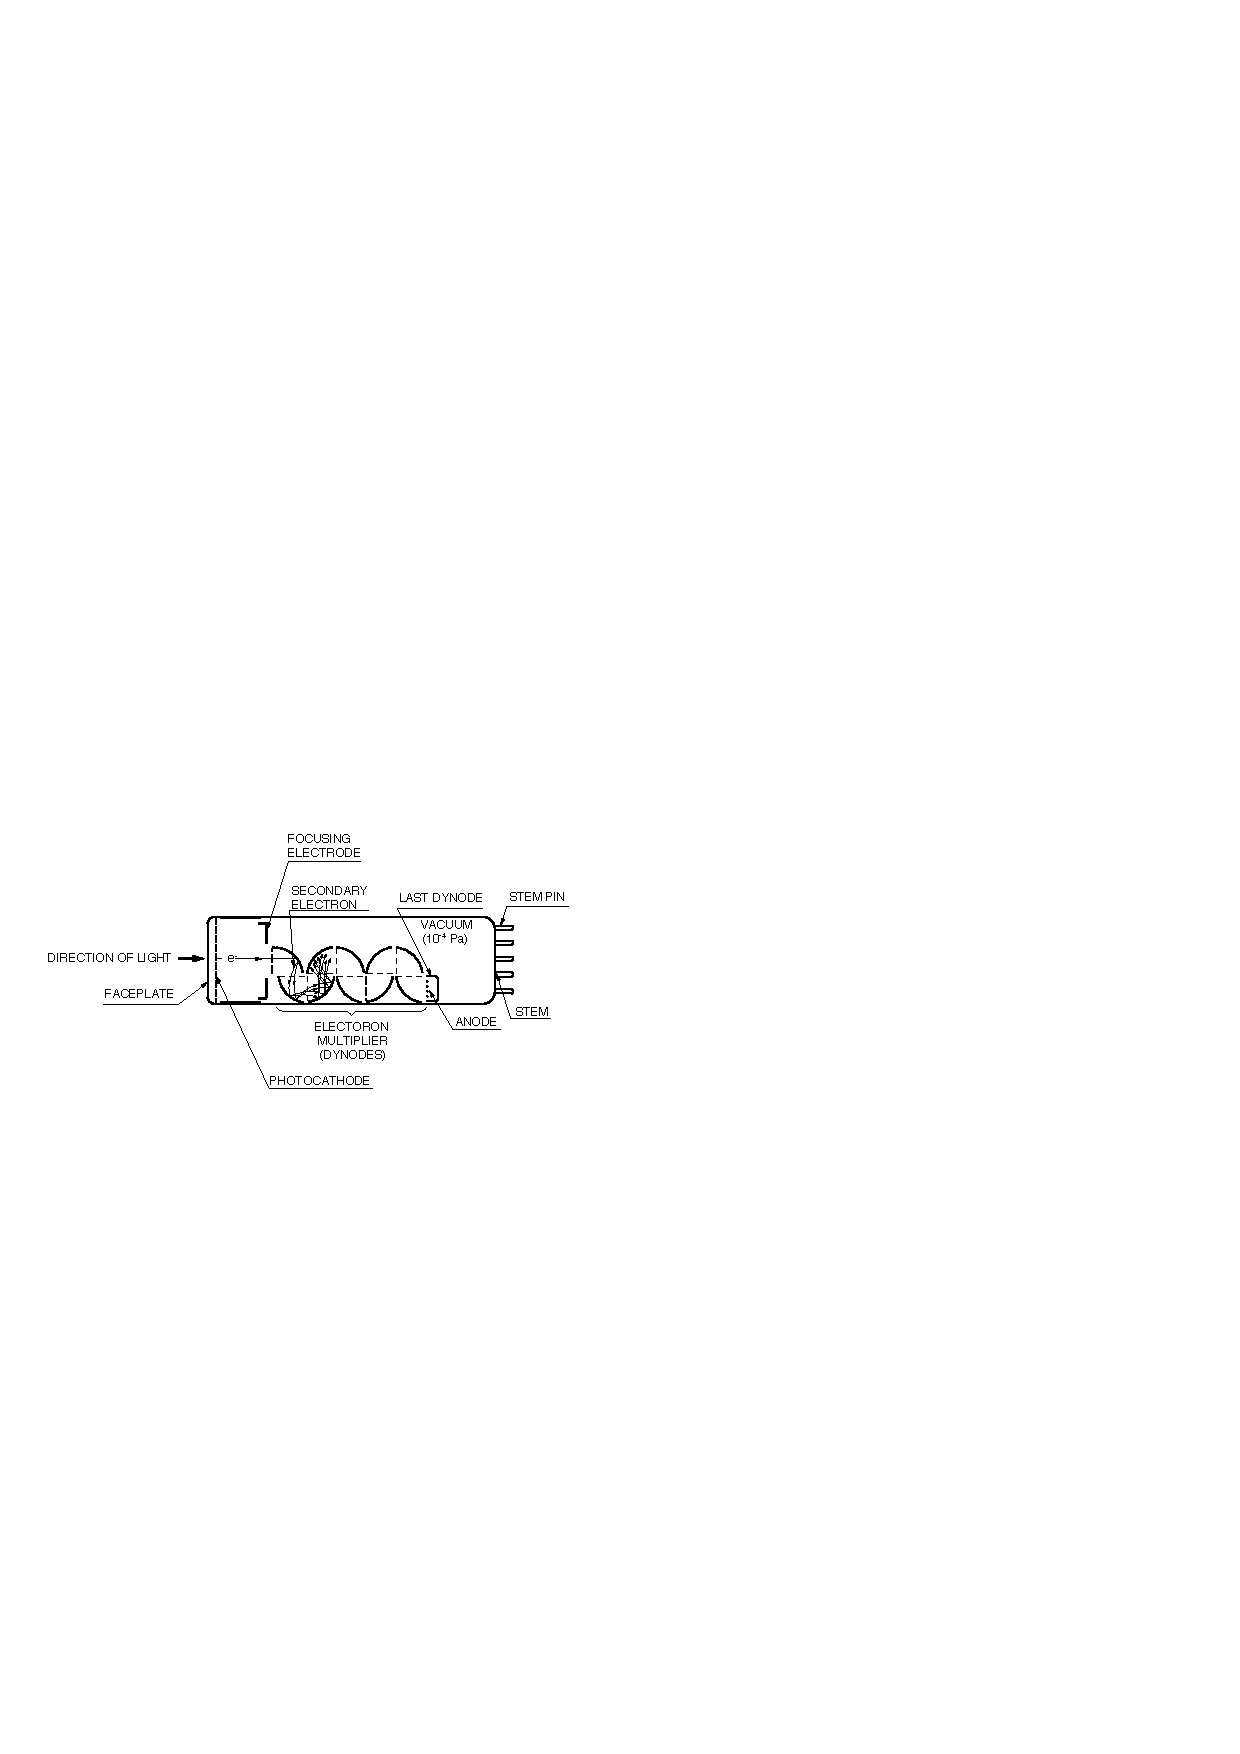
\includegraphics{pmt-schematic}
\caption{Schematische weergave van een \pmt.  Figuur overgenomen uit
\cite{hamamatsu}.}
\label{fig:pmt}
\end{figure}

De \pmt is een verzegelde glazen buis die vacuüm gemaakt
is (\figref{fig:pmt}).  De voorkant van een \pmt bestaat uit een dunne
glaslaag.  Aan de binnenkant van het glas is een zeer dun metaallaagje
opgedampt.  Het laagje is zó dun, dat het doorzichtig is.  Licht dat op de
\pmt valt, gaat door het glas en raakt het metaal.  Het violette licht uit
de scintillator heeft een $E_f$ die hoog genoeg is om elektronen vrij te
maken uit het metaallaagje.  Om er voor te zorgen dat er veel elektronen
beschikbaar zijn wordt het metaalplaatje op een grote negatieve spanning
gezet.  De elektronen staan dan feitelijk te dringen om het metaal te
verlaten.  Het metaallaagje heet de \emph{kathode}\footnote{In een
vacuümbuis is de kathode de pool waar elektronen uit worden vrijgemaakt,
zoals hier gebeurt.} van de \pmt.  De \emph{anode} van de fotobuis wordt
geaard, waardoor er een sterk elektrisch veld in de buis ontstaat.  De
elektronen versnellen richting de anode.  Om een grote versterkingsfactor
te krijgen is de buis opgedeeld in meerdere trappen.  Iedere trap heeft
een \emph{dynode}, een metalen plaatje met een iets minder negatieve
spanning dan de voorgaande dynode.  Dus bij een \pmt met drie dynodes,
zijn de spanningen bijvoorbeeld als volgt: kathode (\SI{-1000}{\volt}),
eerste dynode (\SI{-750}{\volt}), tweede dynode (\SI{-500}{\volt}), derde
dynode (\SI{-250}{\volt}) en kathode (\SI{0}{\volt}).  Zo blijven de
elektronen versnellen van kathode, langs alle dynodes en uiteindelijk naar
de anode.  De versterking treedt op zodra de elektronen een dynode raken.
De grote snelheid waarmee een elektron het metaal intreedt maakt een
aantal elektronen los.  Deze losgeslagen elektronen worden vervolgens
versneld naar de volgende dynode.  Als per dynode per elektron
bijvoorbeeld drie elektronen worden losgeslagen, dan is de totale
versterking in een \pmt met tien dynodes gelijk aan $3^{10} \approx
\num{60000}$.  De hoogspanning die over de \pmt staat bepaalt in grote
mate de versterkingsfactor.  Hoe hoger de spanning, hoe groter de
versterkingsfactor.  De hoogspanning bepaalt namelijk enerzijds de
versnelling van de elektronen en anderzijds het aantal elektronen dat
staat te dringen om de dynode te verlaten.

De \pmt die gebruikt wordt door \hisparc is een 9107B van Electron
Tubes \cite{9107B}.  Deze heeft 11 dynodes en een typische versterking van
\num{3e6} bij \SI{850}{\volt}.  Dat komt overeen met $\num{3.9}^{11}$.  Voor
ieder elektron dat een dynode raakt worden er gemiddeld bijna vier
elektronen vrijgemaakt.


\section{Signaal uit \hisparc detectoren}

Zodra een air shower een detector bereikt gaan één of meerdere deeltjes
door de detector.  Dit veroorzaakt een pulsvormig signaal.  De relatief
lange staart van het signaal wordt veroorzaakt door licht dat via een
aantal reflecties alsnog bij de \pmt terecht komt, maar ook door deeltjes
die een beetje achterliepen in de shower en vrij laat door de detector
gaan.  Het signaal uit de \pmt wordt via kabels met een lengte van
\SI{30}{\meter} naar de \hisparc elektronica geleid.  Alle kabels zijn
precies even lang, om te zorgen dat het signaal uit alle detectoren op
hetzelfde moment bij de elektronica aankomt.

In \figref{fig:traces} staat het signaal van een \hisparc event.  Het
bestaat uit een flinke puls met wat kleinere pieken in de staart.  Dit
signaal is veroorzaakt door meerdere deeltjes die (vrijwel) gelijktijdig
door de detector gingen.  De eerste grote puls is een optelsom van het
licht van meerdere deeltjes.

\begin{figure}
\centering
\documentclass[oneside, 11pt]{article}

\usepackage[T1]{fontenc}
\usepackage[utf8]{inputenc}
\usepackage[dutch]{babel}

\usepackage{fouriernc}
\usepackage[detect-all, load-configurations=binary,
            separate-uncertainty=true, per-mode=symbol,
            retain-explicit-plus, range-phrase={ tot }]{siunitx}

\usepackage{setspace}
\setstretch{1.2}

\setlength{\parskip}{\smallskipamount}
\setlength{\parindent}{0pt}

\usepackage{geometry}
\geometry{marginparwidth=0.5cm, verbose, a4paper, tmargin=3cm, bmargin=3cm, lmargin=2cm, rmargin=2cm}

\usepackage{float}

\usepackage[fleqn]{amsmath}
\numberwithin{equation}{section}
\numberwithin{figure}{section}

\usepackage{graphicx}
\graphicspath{{Figures/}}
\usepackage{subfig}

\usepackage{tikz}
\usetikzlibrary{plotmarks}

\usepackage{fancyhdr}
\pagestyle{fancy}
\fancyhf{}
\rhead{\thepage}
\renewcommand{\footrulewidth}{0pt}
\renewcommand{\headrulewidth}{0pt}

\usepackage{relsize}
\usepackage{xspace}
\usepackage{url}

\newcommand{\figref}[1]{Figuur~\ref{#1}}

\newcommand{\hisparc}{\textsmaller{HiSPARC}\xspace}
\newcommand{\kascade}{\textsmaller{KASCADE}\xspace}
\newcommand{\sapphire}{\textsmaller{SAPPHiRE}\xspace}
\newcommand{\jsparc}{\textsmaller{jSparc}\xspace}
\newcommand{\hdf}{\textsmaller{HDF5}\xspace}
\newcommand{\aires}{\textsmaller{AIRES}\xspace}
\newcommand{\csv}{\textsmaller{CSV}\xspace}
\newcommand{\python}{\textsmaller{PYTHON}\xspace}
\newcommand{\corsika}{\textsmaller{CORSIKA}\xspace}
\newcommand{\labview}{\textsmaller{LabVIEW}\xspace}
\newcommand{\daq}{\textsmaller{DAQ}\xspace}
\newcommand{\adc}{\textsmaller{ADC}\xspace}
\newcommand{\adcs}{\textsmaller{ADC}s\xspace}
\newcommand{\Adcs}{A\textsmaller{DC}s\xspace}
\newcommand{\hi}{\textsc{h i}\xspace}
\newcommand{\hii}{\textsc{h ii}\xspace}
\newcommand{\mip}{\textsmaller{MIP}\xspace}
\newcommand{\hisparcii}{\textsmaller{HiSPARC II}\xspace}
\newcommand{\hisparciii}{\textsmaller{HiSPARC III}\xspace}
\newcommand{\pmt}{\textsmaller{PMT}\xspace}
\newcommand{\pmts}{\textsmaller{PMT}s\xspace}

\DeclareSIUnit{\electronvolt}{\ensuremath{\mathrm{e\!\!\:V}}}

\DeclareSIUnit{\unitsigma}{\ensuremath{\sigma}}
\DeclareSIUnit{\mip}{\textsmaller{MIP}}
\DeclareSIUnit{\adc}{\textsmaller{ADC}}

\DeclareSIUnit{\gauss}{G}
\DeclareSIUnit{\parsec}{pc}
\DeclareSIUnit{\year}{yr}



\title{Pulshoogte en pulsintegraal}
\author{N.G. Schultheiss}
\docwerkblad{2}{PH}
\version{1.0}

\begin{document}

\maketitle

\section{Inleiding}

Elke detector van een \hisparc-station is uitgerust met een
foto-versterker buis (PhotoMultiplier Tube: \pmt). Als er geen deeltjes
door de detector schieten, treedt er geen fluorescentie in de detector
op en ontstaat er geen licht. In dit geval geeft de PMT-buis een
elektrisch signaal van \SI{0}{\milli\volt} aan de \hisparc unit. Als er
wel deeltjes door de detector schieten, treedt er fluorescentie in de
detector op en ontstaat er licht. Dan geeft de PMT-buis een elektrisch
signaal af waarvan het aantal mV afhangt van het aantal deeltjes dat
door de detector is gegaan. In de \hisparc unit wordt het analoge
signaal door middel van een Analoog Digitaal Converter (\adc) omgezet in
een digitaal signaal. De grootte van dit signaal wordt uitgedrukt in
\adcs, de \adc count (een getal zonder eenheid).

Als er een detectorsignaal gemeten wordt, wordt een reeks van deze \adcs
in de \hisparc unit opgeslagen. Als er tegelijkertijd een tweede reeks,
van een andere detector, wordt opgeslagen, worden alle reeksen \adcs van
de \hisparc unit naar de \hisparc server gezonden. Met dergelijke reeks
kan een diagram van het verloop van het signaal tegen de tijd worden
gemaakt. In deze diagrammen zijn van het negatieve maximale signaal de
pulshoogte en het oppervlak, de pulsintegraal, te bepalen. Gedurende de
dag worden alle pulshoogten en pulsintegralen van een station verzameld.
Pulshoogte en pulsintegraal histogrammen zijn op te vragen op:
\url{http://data.hisparc.nl/} door op de stationsnaam te klikken.
Rechtsboven beide histogrammen is een link waarmee de gegevens in een
spreadsheet, zoals Excel, te laden zijn.


\section{De pulsvorm}


\subsection{Pulsen ophalen uit de \hisparc data opslag}

\begin{figure}[ht]
    \centering
    \subfloat{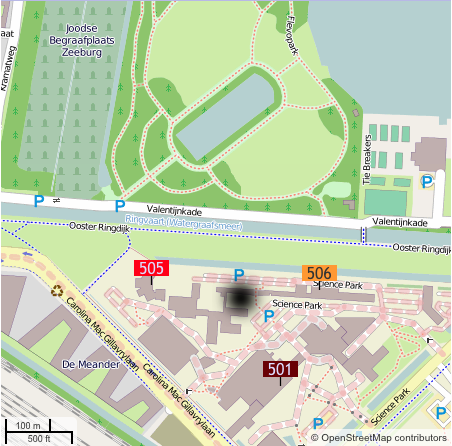
\includegraphics[scale=0.33]{kaart}}
    \subfloat{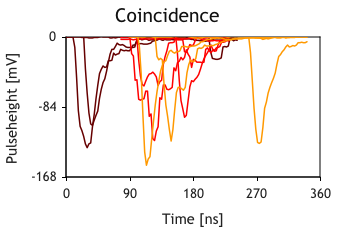
\includegraphics[scale=0.65]{Coincidence}}
    \caption{De plattegrond met de locaties van de meetstations
             en de gemeten pulsen per station.}
    \label{fig:coincidence}
\end{figure}

In de praktijk kunnen we een set pulsen voor een willekeurige
gebeurtenis ophalen met \jsparc%
\footnote{Het interactieve practicum \jsparc kan in de les na aanvraag
van een sessie worden gebruikt, het is ook mogelijk om een willekeurige
set pulsen op te halen op:
\url{http://data.hisparc.nl/media/jsparc/jsparc.html}.%
}. In deze module gaan we uit van de set pulsen die met de stations
uit \figref{fig:coincidence} zijn gemeten.

Op de kaart zijn drie meetstations te zien, een bruin, een rood en een
oranje station%
\footnote{De kleuren van de stations volgen de definitie van de
kleurcode van weerstandjes: bruin: 1, rood: 2, oranje: 3, geel: 4,
groen: 5, blauw: 6, violet: 7, etc. %
}. We zien dat alle stations meerdere pulsen hebben gegeven, dit komt
omdat een station uit meerdere detectoren bestaat. De hoogtes van de
pulsen zijn vergelijkbaar, bijgevolg is het midden van de air-shower
(zwarte vlek in \figref{fig:coincidence}) even ver van alle stations.


\subsection{Eenvoudige pulsvormen}

Het is mogelijk om de diagrammen per detector van een enkel station
te bekijken. In \figref{fig:Eenvoudige-pulsen} zijn de signalen
van vier detectoren van Station 506 te zien. De zwarte puls van detector
1 heeft een vrij steile voorflank. Het verloop van de achterflank
lijkt een halfwaardetijd te hebben (deze loopt exponentieel op). Bij
de blauwe grafiek van detector 4 is iets soortgelijks aan de hand.
Een deeltje lijkt dus herkend te worden aan een steile dalende flank
die wordt gevolgd door een exponentieel oplopende achterflank.

\begin{figure}[ht]
    \centering
    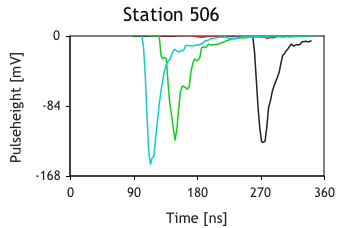
\includegraphics[scale=0.65]{Traces506}
    \caption{Eenvoudige pulsen}
    \label{fig:Eenvoudige-pulsen}
\end{figure}


\begin{minipage}[t]{1\columnwidth}%

\paragraph{Opdracht 1:}

De groene grafiek van detector 3 in \figref{fig:Eenvoudige-pulsen}
heeft een minder vloeiend verloop. Stel een hypothese op waarmee dit
minder vloeiende verloop kan worden verklaard.

\begin{center}
    \rule{\textwidth}{0.3mm}\\
    \rule{\textwidth}{0.3mm}\\
    \rule{\textwidth}{0.3mm}\\
    \rule{\textwidth}{0.3mm}\\
\end{center}
\end{minipage}

\bigskip{}


Meestal zien de grafieken er niet zo mooi uit als in
\figref{fig:Eenvoudige-pulsen}. In \figref{fig:Iets-complexere-pulsen}
zijn andere pulsen van detector 1 en 4 van Station 501 te zien
(respectievelijk zwart en blauw).

\begin{figure}[ht]
    \centering
    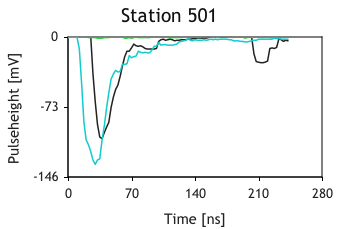
\includegraphics[scale=0.65]{Traces501}
    \caption{Iets complexere pulsen}
    \label{fig:Iets-complexere-pulsen}
\end{figure}


\begin{minipage}[t]{1\columnwidth}%

\paragraph{Opdracht 2:}

Geef een verklaring voor het verloop van de grafiek van detector
1 in \figref{fig:Iets-complexere-pulsen}.

\begin{center}
    \rule{\textwidth}{0.3mm}\\
    \rule{\textwidth}{0.3mm}\\
    \rule{\textwidth}{0.3mm}\\
    \rule{\textwidth}{0.3mm}\\
\end{center}
\end{minipage}

\bigskip{}


\begin{minipage}[t]{1\columnwidth}%

\paragraph{Opdracht 3:}

Bereken de afstand tussen de waargenomen deeltjes in de grafiek
van detector 1 (zwart) in \figref{fig:Iets-complexere-pulsen}.

\begin{center}
    \rule{\textwidth}{0.3mm}\\
    \rule{\textwidth}{0.3mm}\\
    \rule{\textwidth}{0.3mm}\\
    \rule{\textwidth}{0.3mm}\\
\end{center}
\end{minipage}


\subsection{Ingewikkelde pulsvormen}

\begin{figure}[ht]
    \centering
    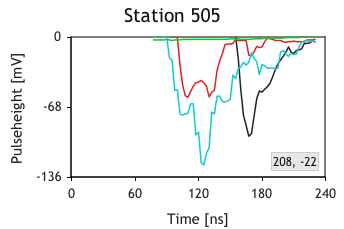
\includegraphics[scale=0.65]{Traces505}
    \caption{Ingewikkelde pulsvormen}
    \label{fig:Ingewikkelde-pulsvormen}
\end{figure}


\bigskip{}

In \figref{fig:Ingewikkelde-pulsvormen} valt het op dat de pulshoogte
van detector 2 (rood) kleiner is dan detector 1 (zwart).

\begin{minipage}[t]{1\columnwidth}%

\paragraph{Opdracht 4:}

Leg met de pulsintegraal (het pulsoppervlak) uit waarom er
waarschijnlijk evenveel deeltjes door detector 1 als door detector
2 zijn gegaan.

\begin{center}
    \rule{\textwidth}{0.3mm}\\
    \rule{\textwidth}{0.3mm}\\
    \rule{\textwidth}{0.3mm}\\
    \rule{\textwidth}{0.3mm}\\
\end{center}
\end{minipage}

\bigskip{}


In \figref{fig:Ingewikkelde-pulsvormen} valt het verder op dat detector
3 (groen) bijna geen puls geeft.

\begin{minipage}[t]{1\columnwidth}%

\paragraph{Opdracht 5:}

Verklaar waarom er binnen een station soms detectoren zijn
die een aantal deeltjes meten terwijl ander detectoren (bijna) niets
meten.

\begin{center}
    \rule{\textwidth}{0.3mm}\\
    \rule{\textwidth}{0.3mm}\\
    \rule{\textwidth}{0.3mm}\\
    \rule{\textwidth}{0.3mm}\\
\end{center}
\end{minipage}
\end{document}

\caption{Een signaal van een event in een \hisparc
detector. % Station 501, detector 4, 1 maart 2012 om 01:54:04.
Het signaal bestaat uit een spanning uit een \pmt.  De (negatieve)
spanning is recht evenredig met de lichtintensiteit die op het venster van
de \pmt valt.  In de staart van het signaal zijn meerdere piekjes te zien.
Dit zijn deeltjes die op een relatief laat tijdstip de detector
bereikten.}
\label{fig:traces}
\end{figure}


\subsection{Pulshoogtehistogram}

Als je alle signalen uit een \hisparc detector bekijkt, dan zie je grote
verschillen.  Dit komt doordate een event veroorzaakt kan worden door één,
twee, drie, of zelfs méér geladen deeltjes die door de detector gaan.  Ook
ontstaan er hoogenergetische fotonen in air showers.  Deze fotonen geven,
met een kleine kans, een relatief zwak signaal in de detectoren.  Maar
omdat het aantal fotonen in een air shower enorm groot is zie je dit terug
in signalen uit de \hisparc detectoren.

In \figref{fig:spectrum_componenten} is een histogram gemaakt van de
componenten van het signaal uit een \hisparc detector.  Er kunnen 1, 2, 3,
of meerdere deeltjes door een detector gaan.  Je zou dus kunnen verwachten
dat in het signaal van een \hisparc detector de stappen duidelijk te zien
zijn, zoals in de bovenste plot.  Doordat het energieverlies van geladen
deeltjes een kansproces is, net als het precieze aantal fotonen dat
uiteindelijk bij de \pmt uitkomt, is het signaal van bv. 2 deeltjes soms
iets kleiner, en soms iets groter.  De componenten zijn dus verbreedt
(middelste plot).  Verder is een afvallende distributie toegevoegd die de
bijdrage van fotonen laat zien.  Fotonen geven over het algemeen een klein
signaal, maar er zijn ontzettend veel fotonen die de plaat raken.  De
energie van de fotonen is zó hoog (gammastraling) dat deze fotonen door
het plastic dringen en door de detector gaan.  In de onderste plot is
tenslotte het totale signaal (zwart) als een optelsom van de verschillende
deeltjescomponenten (grijs) weergegeven.  Dit is het histogram dat op
\url{http://data.hisparc.nl/} en in de \daq software wordt weergegeven.

\begin{figure}
\centering
%% \usepackage{tikz}
% \usetikzlibrary{arrows,pgfplots.groupplots}
% \usepackage{pgfplots}
% \pgfplotsset{compat=1.3}
% \usepackage[detect-family]{siunitx}
% \usepackage[eulergreek]{sansmath}
% \sisetup{text-sf=\sansmath}
% \usepackage{relsize}
%
\pgfkeysifdefined{/artist/width}
    {\pgfkeysgetvalue{/artist/width}{\defaultwidth}}
    {\def\defaultwidth{ .5\linewidth }}
%
%
\begin{sansmath}
\begin{tikzpicture}[font=\sffamily]
\node[inner sep=0pt] (plot) {
    \begin{tikzpicture}[
            inner sep=.3333em,
            font=\sffamily,
            every pin/.style={inner sep=2pt, font={\sffamily\smaller}},
            every label/.style={inner sep=2pt, font={\sffamily\smaller}},
            every pin edge/.style={<-, >=stealth', shorten <=2pt},
            pin distance=2.5ex,
        ]
        \begin{groupplot}[
                xmode=normal,
                ymode=log,
                width=\defaultwidth,
                %
                xmin={ 0 },
                xmax={ 10.5 },
                ymin={ 1 },
                ymax={ 20000.0 },
                %
                group style={rows=3,columns=1,
                             horizontal sep=4pt, vertical sep=4pt},
                %
                tick align=outside,
                max space between ticks=40,
                every tick/.style={},
                axis on top,
                %
                xtick=\empty, ytick=\empty,
                scaled ticks=false,
            ]
            
                
                \nextgroupplot[
                    % Default: empty ticks all round the border of the
                    % multiplot
                            xtick={  },
                            % 'right' means 'top'
                            xtick pos=right,
                            xticklabel=\empty,
                            ytick={  },
                            ytick pos=both,
                            yticklabel=\empty,
                        xticklabel={},
                        yticklabel={},
                    axis equal=false,
                    %
                    title={  },
                    xlabel={  },
                    ylabel={  },
                ]

                

                




    
    % Draw series plot
    \addplot[no markers,solid,const plot] coordinates {
        (0.0, 1e-10)
        (0.111111111111, 1e-10)
        (0.222222222222, 1e-10)
        (0.333333333333, 1e-10)
        (0.444444444444, 1e-10)
        (0.555555555556, 1e-10)
        (0.666666666667, 1e-10)
        (0.777777777778, 1e-10)
        (0.888888888889, 1e-10)
        (1.0, 10000.0)
        (1.11111111111, 1e-10)
        (1.22222222222, 1e-10)
        (1.33333333333, 1e-10)
        (1.44444444444, 1e-10)
        (1.55555555556, 1e-10)
        (1.66666666667, 1e-10)
        (1.77777777778, 1e-10)
        (1.88888888889, 1e-10)
        (2.0, 1250.0)
        (2.11111111111, 1e-10)
        (2.22222222222, 1e-10)
        (2.33333333333, 1e-10)
        (2.44444444444, 1e-10)
        (2.55555555556, 1e-10)
        (2.66666666667, 1e-10)
        (2.77777777778, 1e-10)
        (2.88888888889, 1e-10)
        (3.0, 370.0)
        (3.11111111111, 1e-10)
        (3.22222222222, 1e-10)
        (3.33333333333, 1e-10)
        (3.44444444444, 1e-10)
        (3.55555555556, 1e-10)
        (3.66666666667, 1e-10)
        (3.77777777778, 1e-10)
        (3.88888888889, 1e-10)
        (4.0, 156.0)
        (4.11111111111, 1e-10)
        (4.22222222222, 1e-10)
        (4.33333333333, 1e-10)
        (4.44444444444, 1e-10)
        (4.55555555556, 1e-10)
        (4.66666666667, 1e-10)
        (4.77777777778, 1e-10)
        (4.88888888889, 1e-10)
        (5.0, 80.0)
        (5.11111111111, 1e-10)
        (5.22222222222, 1e-10)
        (5.33333333333, 1e-10)
        (5.44444444444, 1e-10)
        (5.55555555556, 1e-10)
        (5.66666666667, 1e-10)
        (5.77777777778, 1e-10)
        (5.88888888889, 1e-10)
        (6.0, 46.0)
        (6.11111111111, 1e-10)
        (6.22222222222, 1e-10)
        (6.33333333333, 1e-10)
        (6.44444444444, 1e-10)
        (6.55555555556, 1e-10)
        (6.66666666667, 1e-10)
        (6.77777777778, 1e-10)
        (6.88888888889, 1e-10)
        (7.0, 29.0)
        (7.11111111111, 1e-10)
        (7.22222222222, 1e-10)
        (7.33333333333, 1e-10)
        (7.44444444444, 1e-10)
        (7.55555555556, 1e-10)
        (7.66666666667, 1e-10)
        (7.77777777778, 1e-10)
        (7.88888888889, 1e-10)
        (8.0, 19.0)
        (8.11111111111, 1e-10)
        (8.22222222222, 1e-10)
        (8.33333333333, 1e-10)
        (8.44444444444, 1e-10)
        (8.55555555556, 1e-10)
        (8.66666666667, 1e-10)
        (8.77777777778, 1e-10)
        (8.88888888889, 1e-10)
        (9.0, 13.0)
        (9.11111111111, 1e-10)
        (9.22222222222, 1e-10)
        (9.33333333333, 1e-10)
        (9.44444444444, 1e-10)
        (9.55555555556, 1e-10)
        (9.66666666667, 1e-10)
        (9.77777777778, 1e-10)
        (9.88888888889, 1e-10)
        (10.0, 10.0)
        (10.1111111111, 1e-10)
        (10.2222222222, 1e-10)
        (10.3333333333, 1e-10)
        (10.4444444444, 1e-10)
        (10.5555555556, 1e-10)
        (10.6666666667, 1e-10)
        (10.7777777778, 1e-10)
        (10.8888888889, 7.0)
        (11.0, 7.0)
    };










            
                
                \nextgroupplot[
                    % Default: empty ticks all round the border of the
                    % multiplot
                            ytick={  },
                            ytick pos=both,
                            yticklabel=\empty,
                        yticklabel={},
                    axis equal=false,
                    %
                    title={  },
                    xlabel={  },
                    ylabel={  },
                ]

                

                




    
    % Draw series plot
    \addplot[no markers,solid] coordinates {
        (0.0, 153.92227372)
        (0.111111111111, 362.522561425)
        (0.222222222222, 771.96916652)
        (0.333333333333, 1486.26487303)
        (0.444444444444, 2587.16315493)
        (0.555555555556, 4071.76557531)
        (0.666666666667, 5793.92754299)
        (0.777777777778, 7454.09113013)
        (0.888888888889, 8670.57064003)
        (1.0, 9118.68069489)
        (1.11111111111, 8670.57064003)
        (1.22222222222, 7454.09113013)
        (1.33333333333, 5793.92754299)
        (1.44444444444, 4071.76557531)
        (1.55555555556, 2587.16315493)
        (1.66666666667, 1486.26487303)
        (1.77777777778, 771.96916652)
        (1.88888888889, 362.522561425)
        (2.0, 153.92227372)
        (2.11111111111, 59.0879938398)
        (2.22222222222, 20.5082387501)
        (2.33333333333, 6.43559683045)
        (2.44444444444, 1.82591534421)
        (2.55555555556, 0.468385877643)
        (2.66666666667, 0.108632128926)
        (2.77777777778, 0.0227794972095)
        (2.88888888889, 0.00431878239288)
        (3.0, 0.000740303589151)
        (3.11111111111, 0.000114733365352)
        (3.22222222222, 1.60768498148e-05)
        (3.33333333333, 2.03677718568e-06)
        (3.44444444444, 2.33301447554e-07)
        (3.55555555556, 2.41614330805e-08)
        (3.66666666667, 2.26234738064e-09)
        (3.77777777778, 1.9152577881e-10)
        (3.88888888889, 1.46597487689e-11)
        (4.0, 1.01451194079e-12)
        (4.11111111111, 6.34774019248e-14)
        (4.22222222222, 3.59097571415e-15)
        (4.33333333333, 1.83669539688e-16)
        (4.44444444444, 8.49362635388e-18)
        (4.55555555556, 3.55124398316e-19)
        (4.66666666667, 1.34245338615e-20)
        (4.77777777778, 4.58827313598e-22)
        (4.88888888889, 1.41785120428e-23)
        (5.0, 3.96135163036e-25)
        (5.11111111111, 1.00066215954e-26)
        (5.22222222222, 2.285403586e-28)
        (5.33333333333, 4.71921405552e-30)
        (5.44444444444, 8.8106468382e-32)
        (5.55555555556, 1.48722697905e-33)
        (5.66666666667, 2.269750192e-35)
        (5.77777777778, 3.13191677238e-37)
        (5.88888888889, 3.90727256898e-39)
        (6.0, 4.4072587528e-41)
        (6.11111111111, 4.49463815526e-43)
        (6.22222222222, 4.1443102907e-45)
        (6.33333333333, 3.4549450066e-47)
        (6.44444444444, 2.60412219122e-49)
        (6.55555555556, 1.77465085496e-51)
        (6.66666666667, 1.09344220165e-53)
        (6.77777777778, 6.09130134589e-56)
        (6.88888888889, 3.06800231962e-58)
        (7.0, 1.39711651622e-60)
        (7.11111111111, 5.75229187901e-63)
        (7.22222222222, 2.14131494058e-65)
        (7.33333333333, 7.20695025696e-68)
        (7.44444444444, 2.19307683005e-70)
        (7.55555555556, 6.03375280001e-73)
        (7.66666666667, 1.50090265167e-75)
        (7.77777777778, 3.37558370021e-78)
        (7.88888888889, 6.86398905133e-81)
        (8.0, 1.26193105421e-83)
        (8.11111111111, 2.0976161508e-86)
        (8.22222222222, 3.15244670691e-89)
        (8.33333333333, 4.2835203387e-92)
        (8.44444444444, 5.26241698609e-95)
        (8.55555555556, 5.84522223049e-98)
        (8.66666666667, 5.87013570634e-101)
        (8.77777777778, 5.32999252865e-104)
        (8.88888888889, 4.37558781056e-107)
        (9.0, 3.24771231492e-110)
        (9.11111111111, 2.17946573291e-113)
        (9.22222222222, 1.32237272468e-116)
        (9.33333333333, 7.25419232234e-120)
        (9.44444444444, 3.59795388409e-123)
        (9.55555555556, 1.61344239574e-126)
        (9.66666666667, 6.54158036539e-130)
        (9.77777777778, 2.39796722321e-133)
        (9.88888888889, 7.94758440226e-137)
        (10.0, 2.38154284811e-140)
        (10.1111111111, 6.45227687528e-144)
        (10.2222222222, 1.58051614154e-147)
        (10.3333333333, 3.50038827656e-151)
        (10.4444444444, 7.00914186899e-155)
        (10.5555555556, 1.26895092007e-158)
        (10.6666666667, 2.07709396662e-162)
        (10.7777777778, 3.07396422059e-166)
        (10.8888888889, 4.1131336071e-170)
        (11.0, 4.97597477851e-174)
    };

    
    % Draw series plot
    \addplot[no markers,solid] coordinates {
        (0.0, 0.229649734085)
        (0.111111111111, 0.554678944521)
        (0.222222222222, 1.27389339675)
        (0.333333333333, 2.78189135426)
        (0.444444444444, 5.7764752311)
        (0.555555555556, 11.4051588518)
        (0.666666666667, 21.4119112182)
        (0.777777777778, 38.2230379623)
        (0.888888888889, 64.8799702291)
        (1.0, 104.715688962)
        (1.11111111111, 160.704685544)
        (1.22222222222, 234.509800165)
        (1.33333333333, 325.393689499)
        (1.44444444444, 429.311901436)
        (1.55555555556, 538.5827042)
        (1.66666666667, 642.462153761)
        (1.77777777778, 728.71610602)
        (1.88888888889, 785.931797241)
        (2.0, 805.985119354)
        (2.11111111111, 785.931797241)
        (2.22222222222, 728.71610602)
        (2.33333333333, 642.462153761)
        (2.44444444444, 538.5827042)
        (2.55555555556, 429.311901436)
        (2.66666666667, 325.393689499)
        (2.77777777778, 234.509800165)
        (2.88888888889, 160.704685544)
        (3.0, 104.715688962)
        (3.11111111111, 64.8799702291)
        (3.22222222222, 38.2230379623)
        (3.33333333333, 21.4119112182)
        (3.44444444444, 11.4051588518)
        (3.55555555556, 5.7764752311)
        (3.66666666667, 2.78189135426)
        (3.77777777778, 1.27389339675)
        (3.88888888889, 0.554678944521)
        (4.0, 0.229649734085)
        (4.11111111111, 0.0904077967675)
        (4.22222222222, 0.0338424266871)
        (4.33333333333, 0.0120457204547)
        (4.44444444444, 0.004076803096)
        (4.55555555556, 0.00131196534763)
        (4.66666666667, 0.000401458506816)
        (4.77777777778, 0.000116808551358)
        (4.88888888889, 3.23164973459e-05)
        (5.0, 8.50138336591e-06)
        (5.11111111111, 2.12652548093e-06)
        (5.22222222222, 5.05786523338e-07)
        (5.33333333333, 1.14387768611e-07)
        (5.44444444444, 2.45984416844e-08)
        (5.55555555556, 5.02980646621e-09)
        (5.66666666667, 9.77936434544e-10)
        (5.77777777778, 1.80794681692e-10)
        (5.88888888889, 3.17816431941e-11)
        (6.0, 5.31230151375e-12)
        (6.11111111111, 8.4431549181e-13)
        (6.22222222222, 1.27597589979e-13)
        (6.33333333333, 1.83356308913e-14)
        (6.44444444444, 2.50532986901e-15)
        (6.55555555556, 3.25498991247e-16)
        (6.66666666667, 4.02114792942e-17)
        (6.77777777778, 4.7235239932e-18)
        (6.88888888889, 5.27591601528e-19)
        (7.0, 5.60331830443e-20)
        (7.11111111111, 5.65859206877e-21)
        (7.22222222222, 5.43359358538e-22)
        (7.33333333333, 4.96114121303e-23)
        (7.44444444444, 4.30716687919e-24)
        (7.55555555556, 3.55563752319e-25)
        (7.66666666667, 2.79099420782e-26)
        (7.77777777778, 2.0831285064e-27)
        (7.88888888889, 1.47838947221e-28)
        (8.0, 9.97647992037e-30)
        (8.11111111111, 6.40149597436e-31)
        (8.22222222222, 3.9057216853e-32)
        (8.33333333333, 2.26587935085e-33)
        (8.44444444444, 1.24993647816e-34)
        (8.55555555556, 6.55623898803e-36)
        (8.66666666667, 3.26992116145e-37)
        (8.77777777778, 1.5507273979e-38)
        (8.88888888889, 6.99277106935e-40)
        (9.0, 2.99832587954e-41)
        (9.11111111111, 1.22243008171e-42)
        (9.22222222222, 4.73898022126e-44)
        (9.33333333333, 1.74687341723e-45)
        (9.44444444444, 6.12285039955e-47)
        (9.55555555556, 2.04061715371e-48)
        (9.66666666667, 6.46673538326e-50)
        (9.77777777778, 1.94860727458e-51)
        (9.88888888889, 5.58314903981e-53)
        (10.0, 1.52107208256e-54)
        (10.1111111111, 3.94036127229e-56)
        (10.2222222222, 9.70594801366e-58)
        (10.3333333333, 2.27329371945e-59)
        (10.4444444444, 5.06277720105e-61)
        (10.5555555556, 1.07210606206e-62)
        (10.6666666667, 2.1587500469e-64)
        (10.7777777778, 4.13316402572e-66)
        (10.8888888889, 7.52451641199e-68)
        (11.0, 1.30253745127e-69)
    };

    
    % Draw series plot
    \addplot[no markers,solid] coordinates {
        (0.0, 0.000937812466955)
        (0.111111111111, 0.00228422627769)
        (0.222222222222, 0.00537988129367)
        (0.333333333333, 0.0122522743018)
        (0.444444444444, 0.0269818160679)
        (0.555555555556, 0.0574560931581)
        (0.666666666667, 0.118307275935)
        (0.777777777778, 0.235557678581)
        (0.888888888889, 0.453516951753)
        (1.0, 0.844306693786)
        (1.11111111111, 1.51990830541)
        (1.22222222222, 2.64572677319)
        (1.33333333333, 4.4533111941)
        (1.44444444444, 7.24822297306)
        (1.55555555556, 11.4075004229)
        (1.66666666667, 17.3604065152)
        (1.77777777778, 25.5469898644)
        (1.88888888889, 36.3521439234)
        (2.0, 50.0185123513)
        (2.11111111111, 66.5490654038)
        (2.22222222222, 85.6177082753)
        (2.33333333333, 106.511299983)
        (2.44444444444, 128.126280857)
        (2.55555555556, 149.036005815)
        (2.66666666667, 167.631115117)
        (2.77777777778, 182.317565662)
        (2.88888888889, 191.74005211)
        (3.0, 194.987879772)
        (3.11111111111, 191.74005211)
        (3.22222222222, 182.317565662)
        (3.33333333333, 167.631115117)
        (3.44444444444, 149.036005815)
        (3.55555555556, 128.126280857)
        (3.66666666667, 106.511299983)
        (3.77777777778, 85.6177082753)
        (3.88888888889, 66.5490654038)
        (4.0, 50.0185123513)
        (4.11111111111, 36.3521439234)
        (4.22222222222, 25.5469898644)
        (4.33333333333, 17.3604065152)
        (4.44444444444, 11.4075004229)
        (4.55555555556, 7.24822297306)
        (4.66666666667, 4.4533111941)
        (4.77777777778, 2.64572677319)
        (4.88888888889, 1.51990830541)
        (5.0, 0.844306693786)
        (5.11111111111, 0.453516951753)
        (5.22222222222, 0.235557678581)
        (5.33333333333, 0.118307275935)
        (5.44444444444, 0.0574560931581)
        (5.55555555556, 0.0269818160679)
        (5.66666666667, 0.0122522743018)
        (5.77777777778, 0.00537988129367)
        (5.88888888889, 0.00228422627769)
        (6.0, 0.000937812466955)
        (6.11111111111, 0.000372308823193)
        (6.22222222222, 0.000142922664275)
        (6.33333333333, 5.30529242083e-05)
        (6.44444444444, 1.90426768714e-05)
        (6.55555555556, 6.6093251495e-06)
        (6.66666666667, 2.2181794917e-06)
        (6.77777777778, 7.19857778534e-07)
        (6.88888888889, 2.2589528503e-07)
        (7.0, 6.85453627194e-08)
        (7.11111111111, 2.01121935505e-08)
        (7.22222222222, 5.70625596615e-09)
        (7.33333333333, 1.56550156583e-09)
        (7.44444444444, 4.15304093649e-10)
        (7.55555555556, 1.06534277731e-10)
        (7.66666666667, 2.6425485066e-11)
        (7.77777777778, 6.33821575037e-12)
        (7.88888888889, 1.4700141559e-12)
        (8.0, 3.29675340771e-13)
        (8.11111111111, 7.14927263195e-14)
        (8.22222222222, 1.49915902026e-14)
        (8.33333333333, 3.03979288243e-15)
        (8.44444444444, 5.96006139695e-16)
        (8.55555555556, 1.1299726234e-16)
        (8.66666666667, 2.0715506576e-17)
        (8.77777777778, 3.6722618636e-18)
        (8.88888888889, 6.29480346685e-19)
        (9.0, 1.04337675348e-19)
        (9.11111111111, 1.67228612206e-20)
        (9.22222222222, 2.59173422129e-21)
        (9.33333333333, 3.88401402061e-22)
        (9.44444444444, 5.62835604828e-23)
        (9.55555555556, 7.88665394892e-24)
        (9.66666666667, 1.06859824293e-24)
        (9.77777777778, 1.40005976337e-25)
        (9.88888888889, 1.77373665704e-26)
        (10.0, 2.17291209201e-27)
        (10.1111111111, 2.57398267965e-28)
        (10.2222222222, 2.94835335629e-29)
        (10.3333333333, 3.26560680143e-30)
        (10.4444444444, 3.49750786764e-31)
        (10.5555555556, 3.62212936004e-32)
        (10.6666666667, 3.62726813976e-33)
        (10.7777777778, 3.51241492752e-34)
        (10.8888888889, 3.28883749756e-35)
        (11.0, 2.97775844387e-36)
    };

    
    % Draw series plot
    \addplot[no markers,solid] coordinates {
        (0.0, 5.78362179024e-06)
        (0.111111111111, 1.41464249799e-05)
        (0.222222222222, 3.37404874444e-05)
        (0.333333333333, 7.84718407852e-05)
        (0.444444444444, 0.00017796482195)
        (0.555555555556, 0.000393561244013)
        (0.666666666667, 0.000848688507237)
        (0.777777777778, 0.00178460519833)
        (0.888888888889, 0.00365926466908)
        (1.0, 0.00731649916651)
        (1.11111111111, 0.0142649636266)
        (1.22222222222, 0.027120384718)
        (1.33333333333, 0.0502781002379)
        (1.44444444444, 0.0908907546219)
        (1.55555555556, 0.160220615235)
        (1.66666666667, 0.275406963623)
        (1.77777777778, 0.461624951874)
        (1.88888888889, 0.754503866728)
        (2.0, 1.20251776343)
        (2.11111111111, 1.86887118191)
        (2.22222222222, 2.83220751113)
        (2.33333333333, 4.18531942777)
        (2.44444444444, 6.03100911344)
        (2.55555555556, 8.47440462439)
        (2.66666666667, 11.6114443205)
        (2.77777777778, 15.5139050064)
        (2.88888888889, 20.2122121479)
        (3.0, 25.6781897766)
        (3.11111111111, 31.8106685571)
        (3.22222222222, 38.4272251791)
        (3.33333333333, 45.2650589296)
        (3.44444444444, 51.9930136622)
        (3.55555555556, 58.2350869541)
        (3.66666666667, 63.6036884543)
        (3.77777777778, 67.7388331253)
        (3.88888888889, 70.3478707369)
        (4.0, 71.2396929288)
        (4.11111111111, 70.3478707369)
        (4.22222222222, 67.7388331253)
        (4.33333333333, 63.6036884543)
        (4.44444444444, 58.2350869541)
        (4.55555555556, 51.9930136622)
        (4.66666666667, 45.2650589296)
        (4.77777777778, 38.4272251791)
        (4.88888888889, 31.8106685571)
        (5.0, 25.6781897766)
        (5.11111111111, 20.2122121479)
        (5.22222222222, 15.5139050064)
        (5.33333333333, 11.6114443205)
        (5.44444444444, 8.47440462439)
        (5.55555555556, 6.03100911344)
        (5.66666666667, 4.18531942777)
        (5.77777777778, 2.83220751113)
        (5.88888888889, 1.86887118191)
        (6.0, 1.20251776343)
        (6.11111111111, 0.754503866728)
        (6.22222222222, 0.461624951874)
        (6.33333333333, 0.275406963623)
        (6.44444444444, 0.160220615235)
        (6.55555555556, 0.0908907546219)
        (6.66666666667, 0.0502781002379)
        (6.77777777778, 0.027120384718)
        (6.88888888889, 0.0142649636266)
        (7.0, 0.00731649916651)
        (7.11111111111, 0.00365926466908)
        (7.22222222222, 0.00178460519833)
        (7.33333333333, 0.000848688507237)
        (7.44444444444, 0.000393561244013)
        (7.55555555556, 0.00017796482195)
        (7.66666666667, 7.84718407852e-05)
        (7.77777777778, 3.37404874444e-05)
        (7.88888888889, 1.41464249799e-05)
        (8.0, 5.78362179024e-06)
        (8.11111111111, 2.30574303784e-06)
        (8.22222222222, 8.96354416811e-07)
        (8.33333333333, 3.39786762778e-07)
        (8.44444444444, 1.25600389178e-07)
        (8.55555555556, 4.52723825263e-08)
        (8.66666666667, 1.59123217631e-08)
        (8.77777777778, 5.45370433844e-09)
        (8.88888888889, 1.82266755902e-09)
        (9.0, 5.93992790648e-10)
        (9.11111111111, 1.88761195941e-10)
        (9.22222222222, 5.84927584623e-11)
        (9.33333333333, 1.76745889112e-11)
        (9.44444444444, 5.20780094786e-12)
        (9.55555555556, 1.49629514695e-12)
        (9.66666666667, 4.1921613978e-13)
        (9.77777777778, 1.14529287257e-13)
        (9.88888888889, 3.05107552145e-14)
        (10.0, 7.92587453739e-15)
        (10.1111111111, 2.00770206349e-15)
        (10.2222222222, 4.95917202538e-16)
        (10.3333333333, 1.19447459653e-16)
        (10.4444444444, 2.80544977668e-17)
        (10.5555555556, 6.42518911643e-18)
        (10.6666666667, 1.43491827881e-18)
        (10.7777777778, 3.12482900392e-19)
        (10.8888888889, 6.63564558897e-20)
        (11.0, 1.37403546905e-20)
    };

    
    % Draw series plot
    \addplot[no markers,solid] coordinates {
        (0.0, 4.47079031426e-08)
        (0.111111111111, 1.0962896987e-07)
        (0.222222222222, 2.63458754345e-07)
        (0.333333333333, 6.20506312354e-07)
        (0.444444444444, 1.43227378351e-06)
        (0.555555555556, 3.24005326823e-06)
        (0.666666666667, 7.18330864123e-06)
        (0.777777777778, 1.56078532307e-05)
        (0.888888888889, 3.32359492393e-05)
        (1.0, 6.93616267977e-05)
        (1.11111111111, 0.000141865477077)
        (1.22222222222, 0.00028436781711)
        (1.33333333333, 0.000558637948969)
        (1.44444444444, 0.00107554031469)
        (1.55555555556, 0.00202940731739)
        (1.66666666667, 0.00375282245985)
        (1.77777777778, 0.00680131806505)
        (1.88888888889, 0.0120802082249)
        (2.0, 0.0210281963804)
        (2.11111111111, 0.0358736772983)
        (2.22222222222, 0.0599785605856)
        (2.33333333333, 0.0982793894506)
        (2.44444444444, 0.157824757091)
        (2.55555555556, 0.248389983303)
        (2.66666666667, 0.383123944984)
        (2.77777777778, 0.579149629089)
        (2.88888888889, 0.858002469999)
        (3.0, 1.24575478096)
        (3.11111111111, 1.77264943271)
        (3.22222222222, 2.47206233942)
        (3.33333333333, 3.3786425699)
        (3.44444444444, 4.52554981778)
        (3.55555555556, 5.94082444976)
        (3.66666666667, 7.64307915623)
        (3.77777777778, 9.63687585993)
        (3.88888888889, 11.9083184678)
        (4.0, 14.4215149866)
        (4.11111111111, 17.1166038571)
        (4.22222222222, 19.9099689378)
        (4.33333333333, 22.6970719471)
        (4.44444444444, 25.3580208804)
        (4.55555555556, 27.7656052471)
        (4.66666666667, 29.7951244359)
        (4.77777777778, 31.3349878889)
        (4.88888888889, 32.2968471213)
        (5.0, 32.6239838382)
        (5.11111111111, 32.2968471213)
        (5.22222222222, 31.3349878889)
        (5.33333333333, 29.7951244359)
        (5.44444444444, 27.7656052471)
        (5.55555555556, 25.3580208804)
        (5.66666666667, 22.6970719471)
        (5.77777777778, 19.9099689378)
        (5.88888888889, 17.1166038571)
        (6.0, 14.4215149866)
        (6.11111111111, 11.9083184678)
        (6.22222222222, 9.63687585993)
        (6.33333333333, 7.64307915623)
        (6.44444444444, 5.94082444976)
        (6.55555555556, 4.52554981778)
        (6.66666666667, 3.3786425699)
        (6.77777777778, 2.47206233942)
        (6.88888888889, 1.77264943271)
        (7.0, 1.24575478096)
        (7.11111111111, 0.858002469999)
        (7.22222222222, 0.579149629089)
        (7.33333333333, 0.383123944984)
        (7.44444444444, 0.248389983303)
        (7.55555555556, 0.157824757091)
        (7.66666666667, 0.0982793894506)
        (7.77777777778, 0.0599785605856)
        (7.88888888889, 0.0358736772983)
        (8.0, 0.0210281963804)
        (8.11111111111, 0.0120802082249)
        (8.22222222222, 0.00680131806505)
        (8.33333333333, 0.00375282245985)
        (8.44444444444, 0.00202940731739)
        (8.55555555556, 0.00107554031469)
        (8.66666666667, 0.000558637948969)
        (8.77777777778, 0.00028436781711)
        (8.88888888889, 0.000141865477077)
        (9.0, 6.93616267977e-05)
        (9.11111111111, 3.32359492393e-05)
        (9.22222222222, 1.56078532307e-05)
        (9.33333333333, 7.18330864123e-06)
        (9.44444444444, 3.24005326823e-06)
        (9.55555555556, 1.43227378351e-06)
        (9.66666666667, 6.20506312354e-07)
        (9.77777777778, 2.63458754345e-07)
        (9.88888888889, 1.0962896987e-07)
        (10.0, 4.47079031426e-08)
        (10.1111111111, 1.78685593274e-08)
        (10.2222222222, 6.99908140016e-09)
        (10.3333333333, 2.68682152793e-09)
        (10.4444444444, 1.01084103391e-09)
        (10.5555555556, 3.72711828709e-10)
        (10.6666666667, 1.34682062321e-10)
        (10.7777777778, 4.76971696358e-11)
        (10.8888888889, 1.65547157557e-11)
        (11.0, 5.63115027116e-12)
    };

    
    % Draw series plot
    \addplot[no markers,solid] coordinates {
        (0.0, 3.98675366217e-10)
        (0.111111111111, 9.79241727364e-10)
        (0.222222222222, 2.36518788028e-09)
        (0.333333333333, 5.61754555059e-09)
        (0.444444444444, 1.31199682628e-08)
        (0.555555555556, 3.01317385501e-08)
        (0.666666666667, 6.80488547555e-08)
        (0.777777777778, 1.51120253958e-07)
        (0.888888888889, 3.30012015929e-07)
        (1.0, 7.08666748363e-07)
        (1.11111111111, 1.49644094305e-06)
        (1.22222222222, 3.10729390244e-06)
        (1.33333333333, 6.34468854201e-06)
        (1.44444444444, 1.27392396192e-05)
        (1.55555555556, 2.51525447087e-05)
        (1.66666666667, 4.88343685889e-05)
        (1.77777777778, 9.32340281344e-05)
        (1.88888888889, 0.000175036468923)
        (2.0, 0.000323137873835)
        (2.11111111111, 0.000586613977353)
        (2.22222222222, 0.00104718201459)
        (2.33333333333, 0.00183821864357)
        (2.44444444444, 0.00317305341118)
        (2.55555555556, 0.0053859562669)
        (2.66666666667, 0.00898987156084)
        (2.77777777778, 0.0147553452387)
        (2.88888888889, 0.023814994629)
        (3.0, 0.0377969559533)
        (3.11111111111, 0.0589886402469)
        (3.22222222222, 0.0905284678499)
        (3.33333333333, 0.136617765948)
        (3.44444444444, 0.202737651972)
        (3.55555555556, 0.295846795562)
        (3.66666666667, 0.424526251546)
        (3.77777777778, 0.599028460239)
        (3.88888888889, 0.831180959835)
        (4.0, 1.13409370513)
        (4.11111111111, 1.52162458905)
        (4.22222222222, 2.00757287765)
        (4.33333333333, 2.60459585952)
        (4.44444444444, 3.32287952784)
        (4.55555555556, 4.1686369184)
        (4.66666666667, 5.14255291232)
        (4.77777777778, 6.23833498183)
        (4.88888888889, 7.44155743779)
        (5.0, 8.72899428304)
        (5.11111111111, 10.0686166052)
        (5.22222222222, 11.4203817962)
        (5.33333333333, 12.7378657195)
        (5.44444444444, 13.9706924956)
        (5.55555555556, 15.0676118877)
        (5.66666666667, 15.9799766604)
        (5.77777777778, 16.6652978647)
        (5.88888888889, 17.0905187139)
        (6.0, 17.2346565045)
        (6.11111111111, 17.0905187139)
        (6.22222222222, 16.6652978647)
        (6.33333333333, 15.9799766604)
        (6.44444444444, 15.0676118877)
        (6.55555555556, 13.9706924956)
        (6.66666666667, 12.7378657195)
        (6.77777777778, 11.4203817962)
        (6.88888888889, 10.0686166052)
        (7.0, 8.72899428304)
        (7.11111111111, 7.44155743779)
        (7.22222222222, 6.23833498183)
        (7.33333333333, 5.14255291232)
        (7.44444444444, 4.1686369184)
        (7.55555555556, 3.32287952784)
        (7.66666666667, 2.60459585952)
        (7.77777777778, 2.00757287765)
        (7.88888888889, 1.52162458905)
        (8.0, 1.13409370513)
        (8.11111111111, 0.831180959835)
        (8.22222222222, 0.599028460239)
        (8.33333333333, 0.424526251546)
        (8.44444444444, 0.295846795562)
        (8.55555555556, 0.202737651972)
        (8.66666666667, 0.136617765948)
        (8.77777777778, 0.0905284678499)
        (8.88888888889, 0.0589886402469)
        (9.0, 0.0377969559533)
        (9.11111111111, 0.023814994629)
        (9.22222222222, 0.0147553452387)
        (9.33333333333, 0.00898987156084)
        (9.44444444444, 0.0053859562669)
        (9.55555555556, 0.00317305341118)
        (9.66666666667, 0.00183821864357)
        (9.77777777778, 0.00104718201459)
        (9.88888888889, 0.000586613977353)
        (10.0, 0.000323137873835)
        (10.1111111111, 0.000175036468923)
        (10.2222222222, 9.32340281344e-05)
        (10.3333333333, 4.88343685889e-05)
        (10.4444444444, 2.51525447087e-05)
        (10.5555555556, 1.27392396192e-05)
        (10.6666666667, 6.34468854201e-06)
        (10.7777777778, 3.10729390244e-06)
        (10.8888888889, 1.49644094305e-06)
        (11.0, 7.08666748363e-07)
    };

    
    % Draw series plot
    \addplot[no markers,solid] coordinates {
        (0.0, 3.92351303458e-12)
        (0.111111111111, 9.64865248332e-12)
        (0.222222222222, 2.33886720579e-11)
        (0.333333333333, 5.58845552918e-11)
        (0.444444444444, 1.31621055478e-10)
        (0.555555555556, 3.05566875794e-10)
        (0.666666666667, 6.99253282196e-10)
        (0.777777777778, 1.57728469144e-09)
        (0.888888888889, 3.50697764787e-09)
        (1.0, 7.68605065668e-09)
        (1.11111111111, 1.66043095799e-08)
        (1.22222222222, 3.53578408381e-08)
        (1.33333333333, 7.4216075603e-08)
        (1.44444444444, 1.53552740009e-07)
        (1.55555555556, 3.1315870599e-07)
        (1.66666666667, 6.29533353002e-07)
        (1.77777777778, 1.24744191769e-06)
        (1.88888888889, 2.43651594488e-06)
        (2.0, 4.69100090847e-06)
        (2.11111111111, 8.9024411465e-06)
        (2.22222222222, 1.66532898282e-05)
        (2.33333333333, 3.0707064736e-05)
        (2.44444444444, 5.58115268335e-05)
        (2.55555555556, 9.99900620091e-05)
        (2.66666666667, 0.00017657820867)
        (2.77777777778, 0.000307372288563)
        (2.88888888889, 0.000527399422178)
        (3.0, 0.000891993980364)
        (3.11111111111, 0.00148707041125)
        (3.22222222222, 0.00244370330521)
        (3.33333333333, 0.00395833690106)
        (3.44444444444, 0.00632010609442)
        (3.55555555556, 0.00994679843771)
        (3.66666666667, 0.0154308411721)
        (3.77777777778, 0.0235962625478)
        (3.88888888889, 0.0355667492715)
        (4.0, 0.0528436079597)
        (4.11111111111, 0.0773905771434)
        (4.22222222222, 0.111720030069)
        (4.33333333333, 0.158972255978)
        (4.44444444444, 0.222976434068)
        (4.55555555556, 0.308278991183)
        (4.66666666667, 0.420122776955)
        (4.77777777778, 0.564359526913)
        (4.88888888889, 0.747279087894)
        (5.0, 0.975342462786)
        (5.11111111111, 1.25481230939)
        (5.22222222222, 1.5912841738)
        (5.33333333333, 1.98913404948)
        (5.44444444444, 2.45091186717)
        (5.55555555556, 2.97672471058)
        (5.66666666667, 3.56366593491)
        (5.77777777778, 4.20535471365)
        (5.88888888889, 4.89165271454)
        (6.0, 5.60861894156)
        (6.11111111111, 6.33874946914)
        (6.22222222222, 7.06152620293)
        (6.33333333333, 7.75426962254)
        (6.44444444444, 8.39325765899)
        (6.55555555556, 8.95504037173)
        (6.66666666667, 9.41785231327)
        (6.77777777778, 9.76300559812)
        (6.88888888889, 9.97614001644)
        (7.0, 10.0482138291)
        (7.11111111111, 9.97614001644)
        (7.22222222222, 9.76300559812)
        (7.33333333333, 9.41785231327)
        (7.44444444444, 8.95504037173)
        (7.55555555556, 8.39325765899)
        (7.66666666667, 7.75426962254)
        (7.77777777778, 7.06152620293)
        (7.88888888889, 6.33874946914)
        (8.0, 5.60861894156)
        (8.11111111111, 4.89165271454)
        (8.22222222222, 4.20535471365)
        (8.33333333333, 3.56366593491)
        (8.44444444444, 2.97672471058)
        (8.55555555556, 2.45091186717)
        (8.66666666667, 1.98913404948)
        (8.77777777778, 1.5912841738)
        (8.88888888889, 1.25481230939)
        (9.0, 0.975342462786)
        (9.11111111111, 0.747279087894)
        (9.22222222222, 0.564359526913)
        (9.33333333333, 0.420122776955)
        (9.44444444444, 0.308278991183)
        (9.55555555556, 0.222976434068)
        (9.66666666667, 0.158972255978)
        (9.77777777778, 0.111720030069)
        (9.88888888889, 0.0773905771434)
        (10.0, 0.0528436079597)
        (10.1111111111, 0.0355667492715)
        (10.2222222222, 0.0235962625478)
        (10.3333333333, 0.0154308411721)
        (10.4444444444, 0.00994679843771)
        (10.5555555556, 0.00632010609442)
        (10.6666666667, 0.00395833690106)
        (10.7777777778, 0.00244370330521)
        (10.8888888889, 0.00148707041125)
        (11.0, 0.000891993980364)
    };

    
    % Draw series plot
    \addplot[no markers,solid] coordinates {
        (0.0, 4.15023555762e-14)
        (0.111111111111, 1.02153935698e-13)
        (0.222222222222, 2.48294087454e-13)
        (0.333333333333, 5.95945535481e-13)
        (0.444444444444, 1.41245845072e-12)
        (0.555555555556, 3.30577819085e-12)
        (0.666666666667, 7.64012839487e-12)
        (0.777777777778, 1.74363879036e-11)
        (0.888888888889, 3.92953630173e-11)
        (1.0, 8.74490319811e-11)
        (1.11111111111, 1.9217532566e-10)
        (1.22222222222, 4.1703179088e-10)
        (1.33333333333, 8.93654442271e-10)
        (1.44444444444, 1.89103249671e-09)
        (1.55555555556, 3.95145721358e-09)
        (1.66666666667, 8.15350784688e-09)
        (1.77777777778, 1.66134803198e-08)
        (1.88888888889, 3.34276362198e-08)
        (2.0, 6.64170575462e-08)
        (2.11111111111, 1.30311430826e-07)
        (2.22222222222, 2.52472635515e-07)
        (2.33333333333, 4.83031031197e-07)
        (2.44444444444, 9.12566807486e-07)
        (2.55555555556, 1.70248471992e-06)
        (2.66666666667, 3.1363945845e-06)
        (2.77777777778, 5.70567573193e-06)
        (2.88888888889, 1.02497292783e-05)
        (3.0, 1.81822079946e-05)
        (3.11111111111, 3.18500241875e-05)
        (3.22222222222, 5.50936860036e-05)
        (3.33333333333, 9.41071910522e-05)
        (3.44444444444, 0.000158735004935)
        (3.55555555556, 0.000264393958493)
        (3.66666666667, 0.000434869813866)
        (3.77777777778, 0.000706310912246)
        (3.88888888889, 0.00113282151199)
        (4.0, 0.00179413854754)
        (4.11111111111, 0.00280594649195)
        (4.22222222222, 0.00433342925407)
        (4.33333333333, 0.0066086530877)
        (4.44444444444, 0.0099522921621)
        (4.55555555556, 0.0148000164094)
        (4.66666666667, 0.0217335262052)
        (4.77777777778, 0.0315157111524)
        (4.88888888889, 0.0451287127429)
        (5.0, 0.0638127848877)
        (5.11111111111, 0.0891028035299)
        (5.22222222222, 0.122858146079)
        (5.33333333333, 0.167280556392)
        (5.44444444444, 0.224913689163)
        (5.55555555556, 0.29861748408)
        (5.66666666667, 0.391510571367)
        (5.77777777778, 0.506874767415)
        (5.88888888889, 0.648017552444)
        (6.0, 0.818091320012)
        (6.11111111111, 1.01987211638)
        (6.22222222222, 1.25550535581)
        (6.33333333333, 1.52623124181)
        (6.44444444444, 1.83210781379)
        (6.55555555556, 2.17175401317)
        (6.66666666667, 2.54213819921)
        (6.77777777778, 2.9384384522)
        (6.88888888889, 3.35399922997)
        (7.0, 3.7804041974)
        (7.11111111111, 4.20767737656)
        (7.22222222222, 4.6246146139)
        (7.33333333333, 5.01923557625)
        (7.44444444444, 5.37933424649)
        (7.55555555556, 5.69309457828)
        (7.66666666667, 5.94972900816)
        (7.77777777778, 6.14009216594)
        (7.88888888889, 6.25722127169)
        (8.0, 6.29675874495)
        (8.11111111111, 6.25722127169)
        (8.22222222222, 6.14009216594)
        (8.33333333333, 5.94972900816)
        (8.44444444444, 5.69309457828)
        (8.55555555556, 5.37933424649)
        (8.66666666667, 5.01923557625)
        (8.77777777778, 4.6246146139)
        (8.88888888889, 4.20767737656)
        (9.0, 3.7804041974)
        (9.11111111111, 3.35399922997)
        (9.22222222222, 2.9384384522)
        (9.33333333333, 2.54213819921)
        (9.44444444444, 2.17175401317)
        (9.55555555556, 1.83210781379)
        (9.66666666667, 1.52623124181)
        (9.77777777778, 1.25550535581)
        (9.88888888889, 1.01987211638)
        (10.0, 0.818091320012)
        (10.1111111111, 0.648017552444)
        (10.2222222222, 0.506874767415)
        (10.3333333333, 0.391510571367)
        (10.4444444444, 0.29861748408)
        (10.5555555556, 0.224913689163)
        (10.6666666667, 0.167280556392)
        (10.7777777778, 0.122858146079)
        (10.8888888889, 0.0891028035299)
        (11.0, 0.0638127848877)
    };

    
    % Draw series plot
    \addplot[no markers,solid] coordinates {
        (0.0, 4.63882917598e-16)
        (0.111111111111, 1.14260122531e-15)
        (0.222222222222, 2.78302948164e-15)
        (0.333333333333, 6.70313158156e-15)
        (0.444444444444, 1.5965204959e-14)
        (0.555555555556, 3.76017509068e-14)
        (0.666666666667, 8.75746588067e-14)
        (0.777777777778, 2.0169059906e-13)
        (0.888888888889, 4.59335143079e-13)
        (1.0, 1.0344523917e-12)
        (1.11111111111, 2.30371186046e-12)
        (1.22222222222, 5.0732074847e-12)
        (1.33333333333, 1.10477517515e-11)
        (1.44444444444, 2.37904143077e-11)
        (1.55555555556, 5.06602023116e-11)
        (1.66666666667, 1.06676473504e-10)
        (1.77777777778, 2.22129990017e-10)
        (1.88888888889, 4.57385676224e-10)
        (2.0, 9.31311013114e-10)
        (2.11111111111, 1.87518333018e-09)
        (2.22222222222, 3.73361510254e-09)
        (2.33333333333, 7.35109730901e-09)
        (2.44444444444, 1.43123719732e-08)
        (2.55555555556, 2.75554732444e-08)
        (2.66666666667, 5.24615296533e-08)
        (2.77777777778, 9.8766767659e-08)
        (2.88888888889, 1.83872824898e-07)
        (3.0, 3.38501869753e-07)
        (3.11111111111, 6.16227976973e-07)
        (3.22222222222, 1.10932440441e-06)
        (3.33333333333, 1.97475189432e-06)
        (3.44444444444, 3.47618856809e-06)
        (3.55555555556, 6.05105263952e-06)
        (3.66666666667, 1.04158652078e-05)
        (3.77777777778, 1.77295040495e-05)
        (3.88888888889, 2.98424613039e-05)
        (4.0, 4.96717553389e-05)
        (4.11111111111, 8.17562931244e-05)
        (4.22222222222, 0.000133066793716)
        (4.33333333333, 0.000214168211085)
        (4.44444444444, 0.000340860864966)
        (4.55555555556, 0.000536458449979)
        (4.66666666667, 0.000834894990493)
        (4.77777777778, 0.00128488552363)
        (4.88888888889, 0.00195539199551)
        (5.0, 0.00294265973043)
        (5.11111111111, 0.00437908197577)
        (5.22222222222, 0.00644410963262)
        (5.33333333333, 0.00937733824877)
        (5.44444444444, 0.0134937624081)
        (5.55555555556, 0.0192009781086)
        (5.66666666667, 0.0270178298307)
        (5.77777777778, 0.0375936408077)
        (5.88888888889, 0.0517267424731)
        (6.0, 0.0703805549701)
        (6.11111111111, 0.0946950027273)
        (6.22222222222, 0.125990630942)
        (6.33333333333, 0.165762488077)
        (6.44444444444, 0.215660733962)
        (6.55555555556, 0.27745510316)
        (6.66666666667, 0.352980871751)
        (6.77777777778, 0.444064894753)
        (6.88888888889, 0.552431619225)
        (7.0, 0.679590705546)
        (7.11111111111, 0.82670992047)
        (7.22222222222, 0.994479153617)
        (7.33333333333, 1.1829735505)
        (7.44444444444, 1.39152560287)
        (7.55555555556, 1.6186173239)
        (7.66666666667, 1.86180410394)
        (7.77777777778, 2.11768128395)
        (7.88888888889, 2.38190277007)
        (8.0, 2.6492581358)
        (8.11111111111, 2.91381074197)
        (8.22222222222, 3.16909471672)
        (8.33333333333, 3.40836357116)
        (8.44444444444, 3.62487826739)
        (8.55555555556, 3.81221823227)
        (8.66666666667, 3.96459562873)
        (8.77777777778, 4.07715157691)
        (8.88888888889, 4.14621323371)
        (9.0, 4.16949277315)
        (9.11111111111, 4.14621323371)
        (9.22222222222, 4.07715157691)
        (9.33333333333, 3.96459562873)
        (9.44444444444, 3.81221823227)
        (9.55555555556, 3.62487826739)
        (9.66666666667, 3.40836357116)
        (9.77777777778, 3.16909471672)
        (9.88888888889, 2.91381074197)
        (10.0, 2.6492581358)
        (10.1111111111, 2.38190277007)
        (10.2222222222, 2.11768128395)
        (10.3333333333, 1.86180410394)
        (10.4444444444, 1.6186173239)
        (10.5555555556, 1.39152560287)
        (10.6666666667, 1.1829735505)
        (10.7777777778, 0.994479153617)
        (10.8888888889, 0.82670992047)
        (11.0, 0.679590705546)
    };

    
    % Draw series plot
    \addplot[no markers,solid] coordinates {
        (0.0, 5.41535117037e-18)
        (0.111111111111, 1.33461526935e-17)
        (0.222222222222, 3.25618212915e-17)
        (0.333333333333, 7.86474094457e-17)
        (0.444444444444, 1.8805430943e-16)
        (0.555555555556, 4.45148887828e-16)
        (0.666666666667, 1.04315880864e-15)
        (0.777777777778, 2.42001858462e-15)
        (0.888888888889, 5.55789204802e-15)
        (1.0, 1.26364373225e-14)
        (1.11111111111, 2.84421434503e-14)
        (1.22222222222, 6.33757529167e-14)
        (1.33333333333, 1.39799969203e-13)
        (1.44444444444, 3.05291107281e-13)
        (1.55555555556, 6.60000655499e-13)
        (1.66666666667, 1.41253010995e-12)
        (1.77777777778, 2.9927758859e-12)
        (1.88888888889, 6.27731340622e-12)
        (2.0, 1.30345656214e-11)
        (2.11111111111, 2.67943019987e-11)
        (2.22222222222, 5.45269828718e-11)
        (2.33333333333, 1.09850900593e-10)
        (2.44444444444, 2.19088161196e-10)
        (2.55555555556, 4.32570933144e-10)
        (2.66666666667, 8.45510277438e-10)
        (2.77777777778, 1.63607641079e-09)
        (2.88888888889, 3.13408960833e-09)
        (3.0, 5.94350141446e-09)
        (3.11111111111, 1.11582597196e-08)
        (3.22222222222, 2.07383259313e-08)
        (3.33333333333, 3.81569857722e-08)
        (3.44444444444, 6.95020411063e-08)
        (3.55555555556, 1.25326869665e-07)
        (3.66666666667, 2.23724713226e-07)
        (3.77777777778, 3.95372867351e-07)
        (3.88888888889, 6.91708160077e-07)
        (4.0, 1.19801448837e-06)
        (4.11111111111, 2.05411321206e-06)
        (4.22222222222, 3.4866617399e-06)
        (4.33333333333, 5.8589310995e-06)
        (4.44444444444, 9.74653170528e-06)
        (4.55555555556, 1.60511052855e-05)
        (4.66666666667, 2.61687465822e-05)
        (4.77777777778, 4.22361218406e-05)
        (4.88888888889, 6.74851598681e-05)
        (5.0, 0.000106746996063)
        (5.11111111111, 0.000167157619789)
        (5.22222222222, 0.000259131273196)
        (5.33333333333, 0.000397682622217)
        (5.44444444444, 0.000604194173862)
        (5.55555555556, 0.000908739878974)
        (5.66666666667, 0.00135308716753)
        (5.77777777778, 0.00199450485621)
        (5.88888888889, 0.00291049967632)
        (6.0, 0.00420458510108)
        (6.11111111111, 0.00601314772456)
        (6.22222222222, 0.0085134136209)
        (6.33333333333, 0.0119324254327)
        (6.44444444444, 0.0165568173846)
        (6.55555555556, 0.0227430194517)
        (6.66666666667, 0.0309273366232)
        (6.77777777778, 0.0416351424048)
        (6.88888888889, 0.0554882108742)
        (7.0, 0.0732090083074)
        (7.11111111111, 0.095620599098)
        (7.22222222222, 0.123640721674)
        (7.33333333333, 0.158268591253)
        (7.44444444444, 0.20056311983)
        (7.55555555556, 0.251611537159)
        (7.66666666667, 0.312487867129)
        (7.77777777778, 0.384201364636)
        (7.88888888889, 0.467635831825)
        (8.0, 0.563481670068)
        (8.11111111111, 0.672163522025)
        (8.22222222222, 0.793767331545)
        (8.33333333333, 0.927971496547)
        (8.44444444444, 1.07398740141)
        (8.55555555556, 1.23051488472)
        (8.66666666667, 1.3957180356)
        (8.77777777778, 1.56722605836)
        (8.88888888889, 1.74216278398)
        (9.0, 1.91720677323)
        (9.11111111111, 2.08868194009)
        (9.22222222222, 2.25267636804)
        (9.33333333333, 2.40518468037)
        (9.44444444444, 2.54226717127)
        (9.55555555556, 2.66021712113)
        (9.66666666667, 2.75572650648)
        (9.77777777778, 2.82603982309)
        (9.88888888889, 2.86908606217)
        (10.0, 2.88358002517)
        (10.1111111111, 2.86908606217)
        (10.2222222222, 2.82603982309)
        (10.3333333333, 2.75572650648)
        (10.4444444444, 2.66021712113)
        (10.5555555556, 2.54226717127)
        (10.6666666667, 2.40518468037)
        (10.7777777778, 2.25267636804)
        (10.8888888889, 2.08868194009)
        (11.0, 1.91720677323)
    };

    
    % Draw series plot
    \addplot[no markers,solid] coordinates {
        (0.0, 6.54819627178e-20)
        (0.111111111111, 1.61454480405e-19)
        (0.222222222222, 3.94456889481e-19)
        (0.333333333333, 9.54926667028e-19)
        (0.444444444444, 2.29066472833e-18)
        (0.555555555556, 5.44470140024e-18)
        (0.666666666667, 1.28235313195e-17)
        (0.777777777778, 2.99269348338e-17)
        (0.888888888889, 6.92050633319e-17)
        (1.0, 1.58574932141e-16)
        (1.11111111111, 3.60041223915e-16)
        (1.22222222222, 8.10011073069e-16)
        (1.33333333333, 1.80572126972e-15)
        (1.44444444444, 3.98870119069e-15)
        (1.55555555556, 8.7303835385e-15)
        (1.66666666667, 1.89346017535e-14)
        (1.77777777778, 4.06911588459e-14)
        (1.88888888889, 8.66492828904e-14)
        (2.0, 1.82831456365e-13)
        (2.11111111111, 3.82259155396e-13)
        (2.22222222222, 7.91928375536e-13)
        (2.33333333333, 1.62567955626e-12)
        (2.44444444444, 3.30677781652e-12)
        (2.55555555556, 6.66493806558e-12)
        (2.66666666667, 1.33109254757e-11)
        (2.77777777778, 2.63415555114e-11)
        (2.88888888889, 5.16530075384e-11)
        (3.0, 1.00362354579e-10)
        (3.11111111111, 1.93226683985e-10)
        (3.22222222222, 3.68624665509e-10)
        (3.33333333333, 6.96823379357e-10)
        (3.44444444444, 1.30521503143e-09)
        (3.55555555556, 2.42249255643e-09)
        (3.66666666667, 4.45516576075e-09)
        (3.77777777778, 8.11869664866e-09)
        (3.88888888889, 1.46598589959e-08)
        (4.0, 2.6229759168e-08)
        (4.11111111111, 4.65028793661e-08)
        (4.22222222222, 8.16932957261e-08)
        (4.33333333333, 1.4220472309e-07)
        (4.44444444444, 2.45280293006e-07)
        (4.55555555556, 4.19210665103e-07)
        (4.66666666667, 7.09942247278e-07)
        (4.77777777778, 1.19133732968e-06)
        (4.88888888889, 1.98092261896e-06)
        (5.0, 3.26378320284e-06)
        (5.11111111111, 5.3283914939e-06)
        (5.22222222222, 8.6196966283e-06)
        (5.33333333333, 1.38168444094e-05)
        (5.44444444444, 2.19455659077e-05)
        (5.55555555556, 3.45386797981e-05)
        (5.66666666667, 5.38624015365e-05)
        (5.77777777778, 8.32313089277e-05)
        (5.88888888889, 0.000127440881649)
        (6.0, 0.000193353412504)
        (6.11111111111, 0.000290680532271)
        (6.22222222222, 0.000433013148051)
        (6.33333333333, 0.000639156561358)
        (6.44444444444, 0.000934833895987)
        (6.55555555556, 0.00135482337745)
        (6.66666666667, 0.00194559277073)
        (6.77777777778, 0.0027684853986)
        (6.88888888889, 0.00390349441297)
        (7.0, 0.00545363311677)
        (7.11111111111, 0.00754986707998)
        (7.22222222222, 0.0103565170495)
        (7.33333333333, 0.014076969661)
        (7.44444444444, 0.0189594465718)
        (7.55555555556, 0.0253024845824)
        (7.66666666667, 0.0334596745986)
        (7.77777777778, 0.0438431034794)
        (7.88888888889, 0.056924850063)
        (8.0, 0.073235817464)
        (8.11111111111, 0.0933611522483)
        (8.22222222222, 0.117931522114)
        (8.33333333333, 0.147609611127)
        (8.44444444444, 0.183071356541)
        (8.55555555556, 0.224981700229)
        (8.66666666667, 0.273964960258)
        (8.77777777778, 0.330570335268)
        (8.88888888889, 0.395233517156)
        (9.0, 0.4682358774)
        (9.11111111111, 0.549663170941)
        (9.22222222222, 0.639366123739)
        (9.33333333333, 0.736925587043)
        (9.44444444444, 0.841625104988)
        (9.55555555556, 0.952433710765)
        (9.66666666667, 1.06800151027)
        (9.77777777778, 1.18667011818)
        (9.88888888889, 1.30649928795)
        (10.0, 1.42531015582)
        (10.1111111111, 1.54074445445)
        (10.2222222222, 1.65033791849)
        (10.3333333333, 1.7516049931)
        (10.4444444444, 1.84213096216)
        (10.5555555556, 1.91966683159)
        (10.6666666667, 1.98222181525)
        (10.7777777778, 2.0281481378)
        (10.8888888889, 2.0562131208)
        (11.0, 2.06565415259)
    };

    
    % Draw series plot
    \addplot[no markers,solid] coordinates {
        (0.0, 8.15138088654e-22)
        (0.111111111111, 2.01059866649e-21)
        (0.222222222222, 4.91781520847e-21)
        (0.333333333333, 1.19281099387e-20)
        (0.444444444444, 2.86895458094e-20)
        (0.555555555556, 6.84271299317e-20)
        (0.666666666667, 1.61839895125e-19)
        (0.777777777778, 3.79573132649e-19)
        (0.888888888889, 8.82791112033e-19)
        (1.0, 2.03597786446e-18)
        (1.11111111111, 4.65629796637e-18)
        (1.22222222222, 1.05599311834e-17)
        (1.33333333333, 2.3748381894e-17)
        (1.44444444444, 5.29614140773e-17)
        (1.55555555556, 1.17121798458e-16)
        (1.66666666667, 2.5684345591e-16)
        (1.77777777778, 5.58536924371e-16)
        (1.88888888889, 1.20444753083e-15)
        (2.0, 2.57558859978e-15)
        (2.11111111111, 5.46157264552e-15)
        (2.22222222222, 1.14844855929e-14)
        (2.33333333333, 2.39473792418e-14)
        (2.44444444444, 4.95173105498e-14)
        (2.55555555556, 1.01533350442e-13)
        (2.66666666667, 2.06449102078e-13)
        (2.77777777778, 4.16264994956e-13)
        (2.88888888889, 8.32299044771e-13)
        (3.0, 1.65021873446e-12)
        (3.11111111111, 3.24456323164e-12)
        (3.22222222222, 6.32591837029e-12)
        (3.33333333333, 1.22304809831e-11)
        (3.44444444444, 2.34485559271e-11)
        (3.55555555556, 4.45801247356e-11)
        (3.66666666667, 8.40463908803e-11)
        (3.77777777778, 1.57126512113e-10)
        (3.88888888889, 2.91294633472e-10)
        (4.0, 5.35510646245e-10)
        (4.11111111111, 9.76239434985e-10)
        (4.22222222222, 1.7648069143e-09)
        (4.33333333333, 3.1636662274e-09)
        (4.44444444444, 5.62388889479e-09)
        (4.55555555556, 9.91369190942e-09)
        (4.66666666667, 1.73295272789e-08)
        (4.77777777778, 3.00393565707e-08)
        (4.88888888889, 5.16353527305e-08)
        (5.0, 8.80149166921e-08)
        (5.11111111111, 1.48770913058e-07)
        (5.22222222222, 2.49363213904e-07)
        (5.33333333333, 4.14475970377e-07)
        (5.44444444444, 6.83154509366e-07)
        (5.55555555556, 1.11658331465e-06)
        (5.66666666667, 1.80973897805e-06)
        (5.77777777778, 2.9086626812e-06)
        (5.88888888889, 4.63578610557e-06)
        (6.0, 7.32665989808e-06)
        (6.11111111111, 1.14826277773e-05)
        (6.22222222222, 1.78455177945e-05)
        (6.33333333333, 2.75023390998e-05)
        (6.44444444444, 4.20303226068e-05)
        (6.55555555556, 6.36954523859e-05)
        (6.66666666667, 9.57208929827e-05)
        (6.77777777778, 0.000142645366311)
        (6.88888888889, 0.000210795438031)
        (7.0, 0.000308899609302)
        (7.11111111111, 0.000448875727798)
        (7.22222222222, 0.000646826043238)
        (7.33333333333, 0.000924275593242)
        (7.44444444444, 0.00130968871232)
        (7.55555555556, 0.00184029436391)
        (7.66666666667, 0.00256424265172)
        (7.77777777778, 0.00354310118557)
        (7.88888888889, 0.00485467994057)
        (8.0, 0.0065961460452)
        (8.11111111111, 0.00888735513262)
        (8.22222222222, 0.011874283636)
        (8.33333333333, 0.0157323976295)
        (8.44444444444, 0.0206697404155)
        (8.55555555556, 0.0269294660596)
        (8.66666666667, 0.0347914937039)
        (8.77777777778, 0.0445729131237)
        (8.88888888889, 0.056626741977)
        (9.0, 0.0713386265009)
        (9.11111111111, 0.0891210970536)
        (9.22222222222, 0.1104050443)
        (9.33333333333, 0.1356281759)
        (9.44444444444, 0.165220349843)
        (9.55555555556, 0.199585858316)
        (9.66666666667, 0.239082950474)
        (9.77777777778, 0.284001124401)
        (9.88888888889, 0.334536974038)
        (10.0, 0.390769627745)
        (10.1111111111, 0.452637040031)
        (10.2222222222, 0.519914573467)
        (10.3333333333, 0.592197410682)
        (10.4444444444, 0.668888345901)
        (10.5555555556, 0.749192405719)
        (10.6666666667, 0.832119531115)
        (10.7777777778, 0.916496217651)
        (10.8888888889, 1.0009865692)
        (11.0, 1.08412269434)
    };

    
    % Draw series plot
    \addplot[no markers,solid] coordinates {
        (0.0, 1.03976040823e-23)
        (0.111111111111, 2.56547486493e-23)
        (0.222222222222, 6.28109601174e-23)
        (0.333333333333, 1.52593586396e-22)
        (0.444444444444, 3.678496177e-22)
        (0.555555555556, 8.79908510197e-22)
        (0.666666666667, 2.08851648465e-21)
        (0.777777777778, 4.91893945755e-21)
        (0.888888888889, 1.14957742697e-20)
        (1.0, 2.66586503116e-20)
        (1.11111111111, 6.1343883839e-20)
        (1.22222222222, 1.40067558975e-19)
        (1.33333333333, 3.17348925112e-19)
        (1.44444444444, 7.13460088928e-19)
        (1.55555555556, 1.59160581048e-18)
        (1.66666666667, 3.52317753959e-18)
        (1.77777777778, 7.73867702551e-18)
        (1.88888888889, 1.68667766927e-17)
        (2.0, 3.64779689159e-17)
        (2.11111111111, 7.8282084773e-17)
        (2.22222222222, 1.66696813291e-16)
        (2.33333333333, 3.52229229267e-16)
        (2.44444444444, 7.38510488613e-16)
        (2.55555555556, 1.53645952219e-15)
        (2.66666666667, 3.17189468565e-15)
        (2.77777777778, 6.49754918387e-15)
        (2.88888888889, 1.32072856915e-14)
        (3.0, 2.66385603004e-14)
        (3.11111111111, 5.33139802559e-14)
        (3.22222222222, 1.05877735624e-13)
        (3.33333333333, 2.08641820144e-13)
        (3.44444444444, 4.07972848956e-13)
        (3.55555555556, 7.91579138482e-13)
        (3.66666666667, 1.524019765e-12)
        (3.77777777778, 2.91152175159e-12)
        (3.88888888889, 5.51928294914e-12)
        (4.0, 1.03819386775e-11)
        (4.11111111111, 1.93779325558e-11)
        (4.22222222222, 3.58896812399e-11)
        (4.33333333333, 6.59576148747e-11)
        (4.44444444444, 1.20280012432e-10)
        (4.55555555556, 2.1764824344e-10)
        (4.66666666667, 3.90795945251e-10)
        (4.77777777778, 6.96270687196e-10)
        (4.88888888889, 1.23094700256e-09)
        (5.0, 2.1594033896e-09)
        (5.11111111111, 3.75890528504e-09)
        (5.22222222222, 6.49265261805e-09)
        (5.33333333333, 1.11279747557e-08)
        (5.44444444444, 1.89253219744e-08)
        (5.55555555556, 3.19376974372e-08)
        (5.66666666667, 5.34807030829e-08)
        (5.77777777778, 8.88635777048e-08)
        (5.88888888889, 1.4651553011e-07)
        (6.0, 2.39704787272e-07)
        (6.11111111111, 3.89137365989e-07)
        (6.22222222222, 6.26848141393e-07)
        (6.33333333333, 1.00197048909e-06)
        (6.44444444444, 1.58920783985e-06)
        (6.55555555556, 2.50114947795e-06)
        (6.66666666667, 3.90599584188e-06)
        (6.77777777778, 6.05281062164e-06)
        (6.88888888889, 9.30712562336e-06)
        (7.0, 1.4200618035e-05)
        (7.11111111111, 2.14996849805e-05)
        (7.22222222222, 3.22990781624e-05)
        (7.33333333333, 4.81483422244e-05)
        (7.44444444444, 7.12206167674e-05)
        (7.55555555556, 0.000104535380003)
        (7.66666666667, 0.000152248861832)
        (7.77777777778, 0.000220028018352)
        (7.88888888889, 0.000315525962673)
        (8.0, 0.000448978344122)
        (8.11111111111, 0.000633941039569)
        (8.22222222222, 0.000888189269176)
        (8.33333333333, 0.00123479640497)
        (8.44444444444, 0.0017034067791)
        (8.55555555556, 0.00233171016795)
        (8.66666666667, 0.00316711579489)
        (8.77777777778, 0.00426861020347)
        (8.88888888889, 0.00570876590398)
        (9.0, 0.00757584623337)
        (9.11111111111, 0.00997592667441)
        (9.22222222222, 0.013034924672)
        (9.33333333333, 0.0169003999964)
        (9.44444444444, 0.0217429577388)
        (9.55555555556, 0.0277570584715)
        (9.66666666667, 0.0351610178918)
        (9.77777777778, 0.0441959647412)
        (9.88888888889, 0.0551235245322)
        (10.0, 0.0682220111514)
        (10.1111111111, 0.0837809418677)
        (10.2222222222, 0.102093745996)
        (10.3333333333, 0.123448614536)
        (10.4444444444, 0.148117536987)
        (10.5555555556, 0.176343689708)
        (10.6666666667, 0.208327472864)
        (10.7777777778, 0.244211633279)
        (10.8888888889, 0.284066049167)
        (11.0, 0.327872879135)
    };

    
    % Draw series plot
    \addplot[no markers,solid] coordinates {
        (0.0, 1.354117486e-25)
        (0.111111111111, 3.34203564347e-25)
        (0.222222222222, 8.18916225531e-25)
        (0.333333333333, 1.99223947982e-24)
        (0.444444444444, 4.81190756134e-24)
        (0.555555555556, 1.1538960239e-23)
        (0.666666666667, 2.74719663225e-23)
        (0.777777777778, 6.49361418215e-23)
        (0.888888888889, 1.52390145948e-22)
        (1.0, 3.55059351889e-22)
        (1.11111111111, 8.21331906823e-22)
        (1.22222222222, 1.88629711471e-21)
        (1.33333333333, 4.30105676023e-21)
        (1.44444444444, 9.73674765898e-21)
        (1.55555555556, 2.1883980707e-20)
        (1.66666666667, 4.88328868414e-20)
        (1.77777777778, 1.08186268719e-19)
        (1.88888888889, 2.37960872892e-19)
        (2.0, 5.19652034181e-19)
        (2.11111111111, 1.12666130159e-18)
        (2.22222222222, 2.42520129117e-18)
        (2.33333333333, 5.18293630364e-18)
        (2.44444444444, 1.09970859607e-17)
        (2.55555555556, 2.31661058055e-17)
        (2.66666666667, 4.84509301287e-17)
        (2.77777777778, 1.00606228702e-16)
        (2.88888888889, 2.07405986533e-16)
        (3.0, 4.24513370439e-16)
        (3.11111111111, 8.62650992738e-16)
        (3.22222222222, 1.74041391558e-15)
        (3.33333333333, 3.4861304573e-15)
        (3.44444444444, 6.93279551517e-15)
        (3.55555555556, 1.36882148671e-14)
        (3.66666666667, 2.68323619944e-14)
        (3.77777777778, 5.22209372738e-14)
        (3.88888888889, 1.00903002142e-13)
        (4.0, 1.93569612593e-13)
        (4.11111111111, 3.68675214278e-13)
        (4.22222222222, 6.97147010365e-13)
        (4.33333333333, 1.3088156058e-12)
        (4.44444444444, 2.43953036191e-12)
        (4.55555555556, 4.51447921683e-12)
        (4.66666666667, 8.29435760834e-12)
        (4.77777777778, 1.51297419638e-11)
        (4.88888888889, 2.74002139578e-11)
        (5.0, 4.92663121712e-11)
        (5.11111111111, 8.79467554854e-11)
        (5.22222222222, 1.55870259147e-10)
        (5.33333333333, 2.74271296971e-10)
        (5.44444444444, 4.79149600574e-10)
        (5.55555555556, 8.3106610152e-10)
        (5.66666666667, 1.43111216488e-09)
        (5.77777777778, 2.44672661432e-09)
        (5.88888888889, 4.15308563522e-09)
        (6.0, 6.99890331131e-09)
        (6.11111111111, 1.17101583806e-08)
        (6.22222222222, 1.94522217415e-08)
        (6.33333333333, 3.20811052194e-08)
        (6.44444444444, 5.25294797057e-08)
        (6.55555555556, 8.53946266805e-08)
        (6.66666666667, 1.37826160137e-07)
        (6.77777777778, 2.20854593667e-07)
        (6.88888888889, 3.51362075875e-07)
        (7.0, 5.54979574038e-07)
        (7.11111111111, 8.70307611365e-07)
        (7.22222222222, 1.35500916169e-06)
        (7.33333333333, 2.09452403848e-06)
        (7.44444444444, 3.21441639076e-06)
        (7.55555555556, 4.89770458598e-06)
        (7.66666666667, 7.40895072077e-06)
        (7.77777777778, 1.11274203298e-05)
        (7.88888888889, 1.65922754288e-05)
        (8.0, 2.45635464948e-05)
        (8.11111111111, 3.61035460888e-05)
        (8.22222222222, 5.26844338725e-05)
        (8.33333333333, 7.63288013515e-05)
        (8.44444444444, 0.000109791377652)
        (8.55555555556, 0.000156791203721)
        (8.66666666667, 0.000222304790482)
        (8.77777777778, 0.000312931740864)
        (8.88888888889, 0.000437344911906)
        (9.0, 0.000606837216903)
        (9.11111111111, 0.000835976376391)
        (9.22222222222, 0.00114337704695)
        (9.33333333333, 0.00155259649592)
        (9.44444444444, 0.0020931550568)
        (9.55555555556, 0.00280167573161)
        (9.66666666667, 0.00372312830312)
        (9.77777777778, 0.00491215208741)
        (9.88888888889, 0.00643441805315)
        (10.0, 0.0083679757152)
        (10.1111111111, 0.0108045134779)
        (10.2222222222, 0.0138504437388)
        (10.3333333333, 0.0176277071479)
        (10.4444444444, 0.0222741753248)
        (10.5555555556, 0.0279435197118)
        (10.6666666667, 0.0348044079083)
        (10.7777777778, 0.0430388897219)
        (10.8888888889, 0.0528398451312)
        (11.0, 0.0644073870157)
    };










            
                
                \nextgroupplot[
                    % Default: empty ticks all round the border of the
                    % multiplot
                            xtick={  },
                            % 'left' means 'bottom'
                            xtick pos=left,
                            xticklabel=\empty,
                            ytick={  },
                            ytick pos=both,
                            yticklabel=\empty,
                        xticklabel={},
                        yticklabel={},
                    axis equal=false,
                    %
                    title={  },
                    xlabel={  },
                    ylabel={  },
                ]

                

                




    
    % Draw series plot
    \addplot[no markers,lightgray] coordinates {
        (0.0, 153.92227372)
        (0.111111111111, 362.522561425)
        (0.222222222222, 771.96916652)
        (0.333333333333, 1486.26487303)
        (0.444444444444, 2587.16315493)
        (0.555555555556, 4071.76557531)
        (0.666666666667, 5793.92754299)
        (0.777777777778, 7454.09113013)
        (0.888888888889, 8670.57064003)
        (1.0, 9118.68069489)
        (1.11111111111, 8670.57064003)
        (1.22222222222, 7454.09113013)
        (1.33333333333, 5793.92754299)
        (1.44444444444, 4071.76557531)
        (1.55555555556, 2587.16315493)
        (1.66666666667, 1486.26487303)
        (1.77777777778, 771.96916652)
        (1.88888888889, 362.522561425)
        (2.0, 153.92227372)
        (2.11111111111, 59.0879938398)
        (2.22222222222, 20.5082387501)
        (2.33333333333, 6.43559683045)
        (2.44444444444, 1.82591534421)
        (2.55555555556, 0.468385877643)
        (2.66666666667, 0.108632128926)
        (2.77777777778, 0.0227794972095)
        (2.88888888889, 0.00431878239288)
        (3.0, 0.000740303589151)
        (3.11111111111, 0.000114733365352)
        (3.22222222222, 1.60768498148e-05)
        (3.33333333333, 2.03677718568e-06)
        (3.44444444444, 2.33301447554e-07)
        (3.55555555556, 2.41614330805e-08)
        (3.66666666667, 2.26234738064e-09)
        (3.77777777778, 1.9152577881e-10)
        (3.88888888889, 1.46597487689e-11)
        (4.0, 1.01451194079e-12)
        (4.11111111111, 6.34774019248e-14)
        (4.22222222222, 3.59097571415e-15)
        (4.33333333333, 1.83669539688e-16)
        (4.44444444444, 8.49362635388e-18)
        (4.55555555556, 3.55124398316e-19)
        (4.66666666667, 1.34245338615e-20)
        (4.77777777778, 4.58827313598e-22)
        (4.88888888889, 1.41785120428e-23)
        (5.0, 3.96135163036e-25)
        (5.11111111111, 1.00066215954e-26)
        (5.22222222222, 2.285403586e-28)
        (5.33333333333, 4.71921405552e-30)
        (5.44444444444, 8.8106468382e-32)
        (5.55555555556, 1.48722697905e-33)
        (5.66666666667, 2.269750192e-35)
        (5.77777777778, 3.13191677238e-37)
        (5.88888888889, 3.90727256898e-39)
        (6.0, 4.4072587528e-41)
        (6.11111111111, 4.49463815526e-43)
        (6.22222222222, 4.1443102907e-45)
        (6.33333333333, 3.4549450066e-47)
        (6.44444444444, 2.60412219122e-49)
        (6.55555555556, 1.77465085496e-51)
        (6.66666666667, 1.09344220165e-53)
        (6.77777777778, 6.09130134589e-56)
        (6.88888888889, 3.06800231962e-58)
        (7.0, 1.39711651622e-60)
        (7.11111111111, 5.75229187901e-63)
        (7.22222222222, 2.14131494058e-65)
        (7.33333333333, 7.20695025696e-68)
        (7.44444444444, 2.19307683005e-70)
        (7.55555555556, 6.03375280001e-73)
        (7.66666666667, 1.50090265167e-75)
        (7.77777777778, 3.37558370021e-78)
        (7.88888888889, 6.86398905133e-81)
        (8.0, 1.26193105421e-83)
        (8.11111111111, 2.0976161508e-86)
        (8.22222222222, 3.15244670691e-89)
        (8.33333333333, 4.2835203387e-92)
        (8.44444444444, 5.26241698609e-95)
        (8.55555555556, 5.84522223049e-98)
        (8.66666666667, 5.87013570634e-101)
        (8.77777777778, 5.32999252865e-104)
        (8.88888888889, 4.37558781056e-107)
        (9.0, 3.24771231492e-110)
        (9.11111111111, 2.17946573291e-113)
        (9.22222222222, 1.32237272468e-116)
        (9.33333333333, 7.25419232234e-120)
        (9.44444444444, 3.59795388409e-123)
        (9.55555555556, 1.61344239574e-126)
        (9.66666666667, 6.54158036539e-130)
        (9.77777777778, 2.39796722321e-133)
        (9.88888888889, 7.94758440226e-137)
        (10.0, 2.38154284811e-140)
        (10.1111111111, 6.45227687528e-144)
        (10.2222222222, 1.58051614154e-147)
        (10.3333333333, 3.50038827656e-151)
        (10.4444444444, 7.00914186899e-155)
        (10.5555555556, 1.26895092007e-158)
        (10.6666666667, 2.07709396662e-162)
        (10.7777777778, 3.07396422059e-166)
        (10.8888888889, 4.1131336071e-170)
        (11.0, 4.97597477851e-174)
    };

    
    % Draw series plot
    \addplot[no markers,lightgray] coordinates {
        (0.0, 0.229649734085)
        (0.111111111111, 0.554678944521)
        (0.222222222222, 1.27389339675)
        (0.333333333333, 2.78189135426)
        (0.444444444444, 5.7764752311)
        (0.555555555556, 11.4051588518)
        (0.666666666667, 21.4119112182)
        (0.777777777778, 38.2230379623)
        (0.888888888889, 64.8799702291)
        (1.0, 104.715688962)
        (1.11111111111, 160.704685544)
        (1.22222222222, 234.509800165)
        (1.33333333333, 325.393689499)
        (1.44444444444, 429.311901436)
        (1.55555555556, 538.5827042)
        (1.66666666667, 642.462153761)
        (1.77777777778, 728.71610602)
        (1.88888888889, 785.931797241)
        (2.0, 805.985119354)
        (2.11111111111, 785.931797241)
        (2.22222222222, 728.71610602)
        (2.33333333333, 642.462153761)
        (2.44444444444, 538.5827042)
        (2.55555555556, 429.311901436)
        (2.66666666667, 325.393689499)
        (2.77777777778, 234.509800165)
        (2.88888888889, 160.704685544)
        (3.0, 104.715688962)
        (3.11111111111, 64.8799702291)
        (3.22222222222, 38.2230379623)
        (3.33333333333, 21.4119112182)
        (3.44444444444, 11.4051588518)
        (3.55555555556, 5.7764752311)
        (3.66666666667, 2.78189135426)
        (3.77777777778, 1.27389339675)
        (3.88888888889, 0.554678944521)
        (4.0, 0.229649734085)
        (4.11111111111, 0.0904077967675)
        (4.22222222222, 0.0338424266871)
        (4.33333333333, 0.0120457204547)
        (4.44444444444, 0.004076803096)
        (4.55555555556, 0.00131196534763)
        (4.66666666667, 0.000401458506816)
        (4.77777777778, 0.000116808551358)
        (4.88888888889, 3.23164973459e-05)
        (5.0, 8.50138336591e-06)
        (5.11111111111, 2.12652548093e-06)
        (5.22222222222, 5.05786523338e-07)
        (5.33333333333, 1.14387768611e-07)
        (5.44444444444, 2.45984416844e-08)
        (5.55555555556, 5.02980646621e-09)
        (5.66666666667, 9.77936434544e-10)
        (5.77777777778, 1.80794681692e-10)
        (5.88888888889, 3.17816431941e-11)
        (6.0, 5.31230151375e-12)
        (6.11111111111, 8.4431549181e-13)
        (6.22222222222, 1.27597589979e-13)
        (6.33333333333, 1.83356308913e-14)
        (6.44444444444, 2.50532986901e-15)
        (6.55555555556, 3.25498991247e-16)
        (6.66666666667, 4.02114792942e-17)
        (6.77777777778, 4.7235239932e-18)
        (6.88888888889, 5.27591601528e-19)
        (7.0, 5.60331830443e-20)
        (7.11111111111, 5.65859206877e-21)
        (7.22222222222, 5.43359358538e-22)
        (7.33333333333, 4.96114121303e-23)
        (7.44444444444, 4.30716687919e-24)
        (7.55555555556, 3.55563752319e-25)
        (7.66666666667, 2.79099420782e-26)
        (7.77777777778, 2.0831285064e-27)
        (7.88888888889, 1.47838947221e-28)
        (8.0, 9.97647992037e-30)
        (8.11111111111, 6.40149597436e-31)
        (8.22222222222, 3.9057216853e-32)
        (8.33333333333, 2.26587935085e-33)
        (8.44444444444, 1.24993647816e-34)
        (8.55555555556, 6.55623898803e-36)
        (8.66666666667, 3.26992116145e-37)
        (8.77777777778, 1.5507273979e-38)
        (8.88888888889, 6.99277106935e-40)
        (9.0, 2.99832587954e-41)
        (9.11111111111, 1.22243008171e-42)
        (9.22222222222, 4.73898022126e-44)
        (9.33333333333, 1.74687341723e-45)
        (9.44444444444, 6.12285039955e-47)
        (9.55555555556, 2.04061715371e-48)
        (9.66666666667, 6.46673538326e-50)
        (9.77777777778, 1.94860727458e-51)
        (9.88888888889, 5.58314903981e-53)
        (10.0, 1.52107208256e-54)
        (10.1111111111, 3.94036127229e-56)
        (10.2222222222, 9.70594801366e-58)
        (10.3333333333, 2.27329371945e-59)
        (10.4444444444, 5.06277720105e-61)
        (10.5555555556, 1.07210606206e-62)
        (10.6666666667, 2.1587500469e-64)
        (10.7777777778, 4.13316402572e-66)
        (10.8888888889, 7.52451641199e-68)
        (11.0, 1.30253745127e-69)
    };

    
    % Draw series plot
    \addplot[no markers,lightgray] coordinates {
        (0.0, 0.000937812466955)
        (0.111111111111, 0.00228422627769)
        (0.222222222222, 0.00537988129367)
        (0.333333333333, 0.0122522743018)
        (0.444444444444, 0.0269818160679)
        (0.555555555556, 0.0574560931581)
        (0.666666666667, 0.118307275935)
        (0.777777777778, 0.235557678581)
        (0.888888888889, 0.453516951753)
        (1.0, 0.844306693786)
        (1.11111111111, 1.51990830541)
        (1.22222222222, 2.64572677319)
        (1.33333333333, 4.4533111941)
        (1.44444444444, 7.24822297306)
        (1.55555555556, 11.4075004229)
        (1.66666666667, 17.3604065152)
        (1.77777777778, 25.5469898644)
        (1.88888888889, 36.3521439234)
        (2.0, 50.0185123513)
        (2.11111111111, 66.5490654038)
        (2.22222222222, 85.6177082753)
        (2.33333333333, 106.511299983)
        (2.44444444444, 128.126280857)
        (2.55555555556, 149.036005815)
        (2.66666666667, 167.631115117)
        (2.77777777778, 182.317565662)
        (2.88888888889, 191.74005211)
        (3.0, 194.987879772)
        (3.11111111111, 191.74005211)
        (3.22222222222, 182.317565662)
        (3.33333333333, 167.631115117)
        (3.44444444444, 149.036005815)
        (3.55555555556, 128.126280857)
        (3.66666666667, 106.511299983)
        (3.77777777778, 85.6177082753)
        (3.88888888889, 66.5490654038)
        (4.0, 50.0185123513)
        (4.11111111111, 36.3521439234)
        (4.22222222222, 25.5469898644)
        (4.33333333333, 17.3604065152)
        (4.44444444444, 11.4075004229)
        (4.55555555556, 7.24822297306)
        (4.66666666667, 4.4533111941)
        (4.77777777778, 2.64572677319)
        (4.88888888889, 1.51990830541)
        (5.0, 0.844306693786)
        (5.11111111111, 0.453516951753)
        (5.22222222222, 0.235557678581)
        (5.33333333333, 0.118307275935)
        (5.44444444444, 0.0574560931581)
        (5.55555555556, 0.0269818160679)
        (5.66666666667, 0.0122522743018)
        (5.77777777778, 0.00537988129367)
        (5.88888888889, 0.00228422627769)
        (6.0, 0.000937812466955)
        (6.11111111111, 0.000372308823193)
        (6.22222222222, 0.000142922664275)
        (6.33333333333, 5.30529242083e-05)
        (6.44444444444, 1.90426768714e-05)
        (6.55555555556, 6.6093251495e-06)
        (6.66666666667, 2.2181794917e-06)
        (6.77777777778, 7.19857778534e-07)
        (6.88888888889, 2.2589528503e-07)
        (7.0, 6.85453627194e-08)
        (7.11111111111, 2.01121935505e-08)
        (7.22222222222, 5.70625596615e-09)
        (7.33333333333, 1.56550156583e-09)
        (7.44444444444, 4.15304093649e-10)
        (7.55555555556, 1.06534277731e-10)
        (7.66666666667, 2.6425485066e-11)
        (7.77777777778, 6.33821575037e-12)
        (7.88888888889, 1.4700141559e-12)
        (8.0, 3.29675340771e-13)
        (8.11111111111, 7.14927263195e-14)
        (8.22222222222, 1.49915902026e-14)
        (8.33333333333, 3.03979288243e-15)
        (8.44444444444, 5.96006139695e-16)
        (8.55555555556, 1.1299726234e-16)
        (8.66666666667, 2.0715506576e-17)
        (8.77777777778, 3.6722618636e-18)
        (8.88888888889, 6.29480346685e-19)
        (9.0, 1.04337675348e-19)
        (9.11111111111, 1.67228612206e-20)
        (9.22222222222, 2.59173422129e-21)
        (9.33333333333, 3.88401402061e-22)
        (9.44444444444, 5.62835604828e-23)
        (9.55555555556, 7.88665394892e-24)
        (9.66666666667, 1.06859824293e-24)
        (9.77777777778, 1.40005976337e-25)
        (9.88888888889, 1.77373665704e-26)
        (10.0, 2.17291209201e-27)
        (10.1111111111, 2.57398267965e-28)
        (10.2222222222, 2.94835335629e-29)
        (10.3333333333, 3.26560680143e-30)
        (10.4444444444, 3.49750786764e-31)
        (10.5555555556, 3.62212936004e-32)
        (10.6666666667, 3.62726813976e-33)
        (10.7777777778, 3.51241492752e-34)
        (10.8888888889, 3.28883749756e-35)
        (11.0, 2.97775844387e-36)
    };

    
    % Draw series plot
    \addplot[no markers,lightgray] coordinates {
        (0.0, 5.78362179024e-06)
        (0.111111111111, 1.41464249799e-05)
        (0.222222222222, 3.37404874444e-05)
        (0.333333333333, 7.84718407852e-05)
        (0.444444444444, 0.00017796482195)
        (0.555555555556, 0.000393561244013)
        (0.666666666667, 0.000848688507237)
        (0.777777777778, 0.00178460519833)
        (0.888888888889, 0.00365926466908)
        (1.0, 0.00731649916651)
        (1.11111111111, 0.0142649636266)
        (1.22222222222, 0.027120384718)
        (1.33333333333, 0.0502781002379)
        (1.44444444444, 0.0908907546219)
        (1.55555555556, 0.160220615235)
        (1.66666666667, 0.275406963623)
        (1.77777777778, 0.461624951874)
        (1.88888888889, 0.754503866728)
        (2.0, 1.20251776343)
        (2.11111111111, 1.86887118191)
        (2.22222222222, 2.83220751113)
        (2.33333333333, 4.18531942777)
        (2.44444444444, 6.03100911344)
        (2.55555555556, 8.47440462439)
        (2.66666666667, 11.6114443205)
        (2.77777777778, 15.5139050064)
        (2.88888888889, 20.2122121479)
        (3.0, 25.6781897766)
        (3.11111111111, 31.8106685571)
        (3.22222222222, 38.4272251791)
        (3.33333333333, 45.2650589296)
        (3.44444444444, 51.9930136622)
        (3.55555555556, 58.2350869541)
        (3.66666666667, 63.6036884543)
        (3.77777777778, 67.7388331253)
        (3.88888888889, 70.3478707369)
        (4.0, 71.2396929288)
        (4.11111111111, 70.3478707369)
        (4.22222222222, 67.7388331253)
        (4.33333333333, 63.6036884543)
        (4.44444444444, 58.2350869541)
        (4.55555555556, 51.9930136622)
        (4.66666666667, 45.2650589296)
        (4.77777777778, 38.4272251791)
        (4.88888888889, 31.8106685571)
        (5.0, 25.6781897766)
        (5.11111111111, 20.2122121479)
        (5.22222222222, 15.5139050064)
        (5.33333333333, 11.6114443205)
        (5.44444444444, 8.47440462439)
        (5.55555555556, 6.03100911344)
        (5.66666666667, 4.18531942777)
        (5.77777777778, 2.83220751113)
        (5.88888888889, 1.86887118191)
        (6.0, 1.20251776343)
        (6.11111111111, 0.754503866728)
        (6.22222222222, 0.461624951874)
        (6.33333333333, 0.275406963623)
        (6.44444444444, 0.160220615235)
        (6.55555555556, 0.0908907546219)
        (6.66666666667, 0.0502781002379)
        (6.77777777778, 0.027120384718)
        (6.88888888889, 0.0142649636266)
        (7.0, 0.00731649916651)
        (7.11111111111, 0.00365926466908)
        (7.22222222222, 0.00178460519833)
        (7.33333333333, 0.000848688507237)
        (7.44444444444, 0.000393561244013)
        (7.55555555556, 0.00017796482195)
        (7.66666666667, 7.84718407852e-05)
        (7.77777777778, 3.37404874444e-05)
        (7.88888888889, 1.41464249799e-05)
        (8.0, 5.78362179024e-06)
        (8.11111111111, 2.30574303784e-06)
        (8.22222222222, 8.96354416811e-07)
        (8.33333333333, 3.39786762778e-07)
        (8.44444444444, 1.25600389178e-07)
        (8.55555555556, 4.52723825263e-08)
        (8.66666666667, 1.59123217631e-08)
        (8.77777777778, 5.45370433844e-09)
        (8.88888888889, 1.82266755902e-09)
        (9.0, 5.93992790648e-10)
        (9.11111111111, 1.88761195941e-10)
        (9.22222222222, 5.84927584623e-11)
        (9.33333333333, 1.76745889112e-11)
        (9.44444444444, 5.20780094786e-12)
        (9.55555555556, 1.49629514695e-12)
        (9.66666666667, 4.1921613978e-13)
        (9.77777777778, 1.14529287257e-13)
        (9.88888888889, 3.05107552145e-14)
        (10.0, 7.92587453739e-15)
        (10.1111111111, 2.00770206349e-15)
        (10.2222222222, 4.95917202538e-16)
        (10.3333333333, 1.19447459653e-16)
        (10.4444444444, 2.80544977668e-17)
        (10.5555555556, 6.42518911643e-18)
        (10.6666666667, 1.43491827881e-18)
        (10.7777777778, 3.12482900392e-19)
        (10.8888888889, 6.63564558897e-20)
        (11.0, 1.37403546905e-20)
    };

    
    % Draw series plot
    \addplot[no markers,lightgray] coordinates {
        (0.0, 4.47079031426e-08)
        (0.111111111111, 1.0962896987e-07)
        (0.222222222222, 2.63458754345e-07)
        (0.333333333333, 6.20506312354e-07)
        (0.444444444444, 1.43227378351e-06)
        (0.555555555556, 3.24005326823e-06)
        (0.666666666667, 7.18330864123e-06)
        (0.777777777778, 1.56078532307e-05)
        (0.888888888889, 3.32359492393e-05)
        (1.0, 6.93616267977e-05)
        (1.11111111111, 0.000141865477077)
        (1.22222222222, 0.00028436781711)
        (1.33333333333, 0.000558637948969)
        (1.44444444444, 0.00107554031469)
        (1.55555555556, 0.00202940731739)
        (1.66666666667, 0.00375282245985)
        (1.77777777778, 0.00680131806505)
        (1.88888888889, 0.0120802082249)
        (2.0, 0.0210281963804)
        (2.11111111111, 0.0358736772983)
        (2.22222222222, 0.0599785605856)
        (2.33333333333, 0.0982793894506)
        (2.44444444444, 0.157824757091)
        (2.55555555556, 0.248389983303)
        (2.66666666667, 0.383123944984)
        (2.77777777778, 0.579149629089)
        (2.88888888889, 0.858002469999)
        (3.0, 1.24575478096)
        (3.11111111111, 1.77264943271)
        (3.22222222222, 2.47206233942)
        (3.33333333333, 3.3786425699)
        (3.44444444444, 4.52554981778)
        (3.55555555556, 5.94082444976)
        (3.66666666667, 7.64307915623)
        (3.77777777778, 9.63687585993)
        (3.88888888889, 11.9083184678)
        (4.0, 14.4215149866)
        (4.11111111111, 17.1166038571)
        (4.22222222222, 19.9099689378)
        (4.33333333333, 22.6970719471)
        (4.44444444444, 25.3580208804)
        (4.55555555556, 27.7656052471)
        (4.66666666667, 29.7951244359)
        (4.77777777778, 31.3349878889)
        (4.88888888889, 32.2968471213)
        (5.0, 32.6239838382)
        (5.11111111111, 32.2968471213)
        (5.22222222222, 31.3349878889)
        (5.33333333333, 29.7951244359)
        (5.44444444444, 27.7656052471)
        (5.55555555556, 25.3580208804)
        (5.66666666667, 22.6970719471)
        (5.77777777778, 19.9099689378)
        (5.88888888889, 17.1166038571)
        (6.0, 14.4215149866)
        (6.11111111111, 11.9083184678)
        (6.22222222222, 9.63687585993)
        (6.33333333333, 7.64307915623)
        (6.44444444444, 5.94082444976)
        (6.55555555556, 4.52554981778)
        (6.66666666667, 3.3786425699)
        (6.77777777778, 2.47206233942)
        (6.88888888889, 1.77264943271)
        (7.0, 1.24575478096)
        (7.11111111111, 0.858002469999)
        (7.22222222222, 0.579149629089)
        (7.33333333333, 0.383123944984)
        (7.44444444444, 0.248389983303)
        (7.55555555556, 0.157824757091)
        (7.66666666667, 0.0982793894506)
        (7.77777777778, 0.0599785605856)
        (7.88888888889, 0.0358736772983)
        (8.0, 0.0210281963804)
        (8.11111111111, 0.0120802082249)
        (8.22222222222, 0.00680131806505)
        (8.33333333333, 0.00375282245985)
        (8.44444444444, 0.00202940731739)
        (8.55555555556, 0.00107554031469)
        (8.66666666667, 0.000558637948969)
        (8.77777777778, 0.00028436781711)
        (8.88888888889, 0.000141865477077)
        (9.0, 6.93616267977e-05)
        (9.11111111111, 3.32359492393e-05)
        (9.22222222222, 1.56078532307e-05)
        (9.33333333333, 7.18330864123e-06)
        (9.44444444444, 3.24005326823e-06)
        (9.55555555556, 1.43227378351e-06)
        (9.66666666667, 6.20506312354e-07)
        (9.77777777778, 2.63458754345e-07)
        (9.88888888889, 1.0962896987e-07)
        (10.0, 4.47079031426e-08)
        (10.1111111111, 1.78685593274e-08)
        (10.2222222222, 6.99908140016e-09)
        (10.3333333333, 2.68682152793e-09)
        (10.4444444444, 1.01084103391e-09)
        (10.5555555556, 3.72711828709e-10)
        (10.6666666667, 1.34682062321e-10)
        (10.7777777778, 4.76971696358e-11)
        (10.8888888889, 1.65547157557e-11)
        (11.0, 5.63115027116e-12)
    };

    
    % Draw series plot
    \addplot[no markers,lightgray] coordinates {
        (0.0, 3.98675366217e-10)
        (0.111111111111, 9.79241727364e-10)
        (0.222222222222, 2.36518788028e-09)
        (0.333333333333, 5.61754555059e-09)
        (0.444444444444, 1.31199682628e-08)
        (0.555555555556, 3.01317385501e-08)
        (0.666666666667, 6.80488547555e-08)
        (0.777777777778, 1.51120253958e-07)
        (0.888888888889, 3.30012015929e-07)
        (1.0, 7.08666748363e-07)
        (1.11111111111, 1.49644094305e-06)
        (1.22222222222, 3.10729390244e-06)
        (1.33333333333, 6.34468854201e-06)
        (1.44444444444, 1.27392396192e-05)
        (1.55555555556, 2.51525447087e-05)
        (1.66666666667, 4.88343685889e-05)
        (1.77777777778, 9.32340281344e-05)
        (1.88888888889, 0.000175036468923)
        (2.0, 0.000323137873835)
        (2.11111111111, 0.000586613977353)
        (2.22222222222, 0.00104718201459)
        (2.33333333333, 0.00183821864357)
        (2.44444444444, 0.00317305341118)
        (2.55555555556, 0.0053859562669)
        (2.66666666667, 0.00898987156084)
        (2.77777777778, 0.0147553452387)
        (2.88888888889, 0.023814994629)
        (3.0, 0.0377969559533)
        (3.11111111111, 0.0589886402469)
        (3.22222222222, 0.0905284678499)
        (3.33333333333, 0.136617765948)
        (3.44444444444, 0.202737651972)
        (3.55555555556, 0.295846795562)
        (3.66666666667, 0.424526251546)
        (3.77777777778, 0.599028460239)
        (3.88888888889, 0.831180959835)
        (4.0, 1.13409370513)
        (4.11111111111, 1.52162458905)
        (4.22222222222, 2.00757287765)
        (4.33333333333, 2.60459585952)
        (4.44444444444, 3.32287952784)
        (4.55555555556, 4.1686369184)
        (4.66666666667, 5.14255291232)
        (4.77777777778, 6.23833498183)
        (4.88888888889, 7.44155743779)
        (5.0, 8.72899428304)
        (5.11111111111, 10.0686166052)
        (5.22222222222, 11.4203817962)
        (5.33333333333, 12.7378657195)
        (5.44444444444, 13.9706924956)
        (5.55555555556, 15.0676118877)
        (5.66666666667, 15.9799766604)
        (5.77777777778, 16.6652978647)
        (5.88888888889, 17.0905187139)
        (6.0, 17.2346565045)
        (6.11111111111, 17.0905187139)
        (6.22222222222, 16.6652978647)
        (6.33333333333, 15.9799766604)
        (6.44444444444, 15.0676118877)
        (6.55555555556, 13.9706924956)
        (6.66666666667, 12.7378657195)
        (6.77777777778, 11.4203817962)
        (6.88888888889, 10.0686166052)
        (7.0, 8.72899428304)
        (7.11111111111, 7.44155743779)
        (7.22222222222, 6.23833498183)
        (7.33333333333, 5.14255291232)
        (7.44444444444, 4.1686369184)
        (7.55555555556, 3.32287952784)
        (7.66666666667, 2.60459585952)
        (7.77777777778, 2.00757287765)
        (7.88888888889, 1.52162458905)
        (8.0, 1.13409370513)
        (8.11111111111, 0.831180959835)
        (8.22222222222, 0.599028460239)
        (8.33333333333, 0.424526251546)
        (8.44444444444, 0.295846795562)
        (8.55555555556, 0.202737651972)
        (8.66666666667, 0.136617765948)
        (8.77777777778, 0.0905284678499)
        (8.88888888889, 0.0589886402469)
        (9.0, 0.0377969559533)
        (9.11111111111, 0.023814994629)
        (9.22222222222, 0.0147553452387)
        (9.33333333333, 0.00898987156084)
        (9.44444444444, 0.0053859562669)
        (9.55555555556, 0.00317305341118)
        (9.66666666667, 0.00183821864357)
        (9.77777777778, 0.00104718201459)
        (9.88888888889, 0.000586613977353)
        (10.0, 0.000323137873835)
        (10.1111111111, 0.000175036468923)
        (10.2222222222, 9.32340281344e-05)
        (10.3333333333, 4.88343685889e-05)
        (10.4444444444, 2.51525447087e-05)
        (10.5555555556, 1.27392396192e-05)
        (10.6666666667, 6.34468854201e-06)
        (10.7777777778, 3.10729390244e-06)
        (10.8888888889, 1.49644094305e-06)
        (11.0, 7.08666748363e-07)
    };

    
    % Draw series plot
    \addplot[no markers,lightgray] coordinates {
        (0.0, 3.92351303458e-12)
        (0.111111111111, 9.64865248332e-12)
        (0.222222222222, 2.33886720579e-11)
        (0.333333333333, 5.58845552918e-11)
        (0.444444444444, 1.31621055478e-10)
        (0.555555555556, 3.05566875794e-10)
        (0.666666666667, 6.99253282196e-10)
        (0.777777777778, 1.57728469144e-09)
        (0.888888888889, 3.50697764787e-09)
        (1.0, 7.68605065668e-09)
        (1.11111111111, 1.66043095799e-08)
        (1.22222222222, 3.53578408381e-08)
        (1.33333333333, 7.4216075603e-08)
        (1.44444444444, 1.53552740009e-07)
        (1.55555555556, 3.1315870599e-07)
        (1.66666666667, 6.29533353002e-07)
        (1.77777777778, 1.24744191769e-06)
        (1.88888888889, 2.43651594488e-06)
        (2.0, 4.69100090847e-06)
        (2.11111111111, 8.9024411465e-06)
        (2.22222222222, 1.66532898282e-05)
        (2.33333333333, 3.0707064736e-05)
        (2.44444444444, 5.58115268335e-05)
        (2.55555555556, 9.99900620091e-05)
        (2.66666666667, 0.00017657820867)
        (2.77777777778, 0.000307372288563)
        (2.88888888889, 0.000527399422178)
        (3.0, 0.000891993980364)
        (3.11111111111, 0.00148707041125)
        (3.22222222222, 0.00244370330521)
        (3.33333333333, 0.00395833690106)
        (3.44444444444, 0.00632010609442)
        (3.55555555556, 0.00994679843771)
        (3.66666666667, 0.0154308411721)
        (3.77777777778, 0.0235962625478)
        (3.88888888889, 0.0355667492715)
        (4.0, 0.0528436079597)
        (4.11111111111, 0.0773905771434)
        (4.22222222222, 0.111720030069)
        (4.33333333333, 0.158972255978)
        (4.44444444444, 0.222976434068)
        (4.55555555556, 0.308278991183)
        (4.66666666667, 0.420122776955)
        (4.77777777778, 0.564359526913)
        (4.88888888889, 0.747279087894)
        (5.0, 0.975342462786)
        (5.11111111111, 1.25481230939)
        (5.22222222222, 1.5912841738)
        (5.33333333333, 1.98913404948)
        (5.44444444444, 2.45091186717)
        (5.55555555556, 2.97672471058)
        (5.66666666667, 3.56366593491)
        (5.77777777778, 4.20535471365)
        (5.88888888889, 4.89165271454)
        (6.0, 5.60861894156)
        (6.11111111111, 6.33874946914)
        (6.22222222222, 7.06152620293)
        (6.33333333333, 7.75426962254)
        (6.44444444444, 8.39325765899)
        (6.55555555556, 8.95504037173)
        (6.66666666667, 9.41785231327)
        (6.77777777778, 9.76300559812)
        (6.88888888889, 9.97614001644)
        (7.0, 10.0482138291)
        (7.11111111111, 9.97614001644)
        (7.22222222222, 9.76300559812)
        (7.33333333333, 9.41785231327)
        (7.44444444444, 8.95504037173)
        (7.55555555556, 8.39325765899)
        (7.66666666667, 7.75426962254)
        (7.77777777778, 7.06152620293)
        (7.88888888889, 6.33874946914)
        (8.0, 5.60861894156)
        (8.11111111111, 4.89165271454)
        (8.22222222222, 4.20535471365)
        (8.33333333333, 3.56366593491)
        (8.44444444444, 2.97672471058)
        (8.55555555556, 2.45091186717)
        (8.66666666667, 1.98913404948)
        (8.77777777778, 1.5912841738)
        (8.88888888889, 1.25481230939)
        (9.0, 0.975342462786)
        (9.11111111111, 0.747279087894)
        (9.22222222222, 0.564359526913)
        (9.33333333333, 0.420122776955)
        (9.44444444444, 0.308278991183)
        (9.55555555556, 0.222976434068)
        (9.66666666667, 0.158972255978)
        (9.77777777778, 0.111720030069)
        (9.88888888889, 0.0773905771434)
        (10.0, 0.0528436079597)
        (10.1111111111, 0.0355667492715)
        (10.2222222222, 0.0235962625478)
        (10.3333333333, 0.0154308411721)
        (10.4444444444, 0.00994679843771)
        (10.5555555556, 0.00632010609442)
        (10.6666666667, 0.00395833690106)
        (10.7777777778, 0.00244370330521)
        (10.8888888889, 0.00148707041125)
        (11.0, 0.000891993980364)
    };

    
    % Draw series plot
    \addplot[no markers,lightgray] coordinates {
        (0.0, 4.15023555762e-14)
        (0.111111111111, 1.02153935698e-13)
        (0.222222222222, 2.48294087454e-13)
        (0.333333333333, 5.95945535481e-13)
        (0.444444444444, 1.41245845072e-12)
        (0.555555555556, 3.30577819085e-12)
        (0.666666666667, 7.64012839487e-12)
        (0.777777777778, 1.74363879036e-11)
        (0.888888888889, 3.92953630173e-11)
        (1.0, 8.74490319811e-11)
        (1.11111111111, 1.9217532566e-10)
        (1.22222222222, 4.1703179088e-10)
        (1.33333333333, 8.93654442271e-10)
        (1.44444444444, 1.89103249671e-09)
        (1.55555555556, 3.95145721358e-09)
        (1.66666666667, 8.15350784688e-09)
        (1.77777777778, 1.66134803198e-08)
        (1.88888888889, 3.34276362198e-08)
        (2.0, 6.64170575462e-08)
        (2.11111111111, 1.30311430826e-07)
        (2.22222222222, 2.52472635515e-07)
        (2.33333333333, 4.83031031197e-07)
        (2.44444444444, 9.12566807486e-07)
        (2.55555555556, 1.70248471992e-06)
        (2.66666666667, 3.1363945845e-06)
        (2.77777777778, 5.70567573193e-06)
        (2.88888888889, 1.02497292783e-05)
        (3.0, 1.81822079946e-05)
        (3.11111111111, 3.18500241875e-05)
        (3.22222222222, 5.50936860036e-05)
        (3.33333333333, 9.41071910522e-05)
        (3.44444444444, 0.000158735004935)
        (3.55555555556, 0.000264393958493)
        (3.66666666667, 0.000434869813866)
        (3.77777777778, 0.000706310912246)
        (3.88888888889, 0.00113282151199)
        (4.0, 0.00179413854754)
        (4.11111111111, 0.00280594649195)
        (4.22222222222, 0.00433342925407)
        (4.33333333333, 0.0066086530877)
        (4.44444444444, 0.0099522921621)
        (4.55555555556, 0.0148000164094)
        (4.66666666667, 0.0217335262052)
        (4.77777777778, 0.0315157111524)
        (4.88888888889, 0.0451287127429)
        (5.0, 0.0638127848877)
        (5.11111111111, 0.0891028035299)
        (5.22222222222, 0.122858146079)
        (5.33333333333, 0.167280556392)
        (5.44444444444, 0.224913689163)
        (5.55555555556, 0.29861748408)
        (5.66666666667, 0.391510571367)
        (5.77777777778, 0.506874767415)
        (5.88888888889, 0.648017552444)
        (6.0, 0.818091320012)
        (6.11111111111, 1.01987211638)
        (6.22222222222, 1.25550535581)
        (6.33333333333, 1.52623124181)
        (6.44444444444, 1.83210781379)
        (6.55555555556, 2.17175401317)
        (6.66666666667, 2.54213819921)
        (6.77777777778, 2.9384384522)
        (6.88888888889, 3.35399922997)
        (7.0, 3.7804041974)
        (7.11111111111, 4.20767737656)
        (7.22222222222, 4.6246146139)
        (7.33333333333, 5.01923557625)
        (7.44444444444, 5.37933424649)
        (7.55555555556, 5.69309457828)
        (7.66666666667, 5.94972900816)
        (7.77777777778, 6.14009216594)
        (7.88888888889, 6.25722127169)
        (8.0, 6.29675874495)
        (8.11111111111, 6.25722127169)
        (8.22222222222, 6.14009216594)
        (8.33333333333, 5.94972900816)
        (8.44444444444, 5.69309457828)
        (8.55555555556, 5.37933424649)
        (8.66666666667, 5.01923557625)
        (8.77777777778, 4.6246146139)
        (8.88888888889, 4.20767737656)
        (9.0, 3.7804041974)
        (9.11111111111, 3.35399922997)
        (9.22222222222, 2.9384384522)
        (9.33333333333, 2.54213819921)
        (9.44444444444, 2.17175401317)
        (9.55555555556, 1.83210781379)
        (9.66666666667, 1.52623124181)
        (9.77777777778, 1.25550535581)
        (9.88888888889, 1.01987211638)
        (10.0, 0.818091320012)
        (10.1111111111, 0.648017552444)
        (10.2222222222, 0.506874767415)
        (10.3333333333, 0.391510571367)
        (10.4444444444, 0.29861748408)
        (10.5555555556, 0.224913689163)
        (10.6666666667, 0.167280556392)
        (10.7777777778, 0.122858146079)
        (10.8888888889, 0.0891028035299)
        (11.0, 0.0638127848877)
    };

    
    % Draw series plot
    \addplot[no markers,lightgray] coordinates {
        (0.0, 4.63882917598e-16)
        (0.111111111111, 1.14260122531e-15)
        (0.222222222222, 2.78302948164e-15)
        (0.333333333333, 6.70313158156e-15)
        (0.444444444444, 1.5965204959e-14)
        (0.555555555556, 3.76017509068e-14)
        (0.666666666667, 8.75746588067e-14)
        (0.777777777778, 2.0169059906e-13)
        (0.888888888889, 4.59335143079e-13)
        (1.0, 1.0344523917e-12)
        (1.11111111111, 2.30371186046e-12)
        (1.22222222222, 5.0732074847e-12)
        (1.33333333333, 1.10477517515e-11)
        (1.44444444444, 2.37904143077e-11)
        (1.55555555556, 5.06602023116e-11)
        (1.66666666667, 1.06676473504e-10)
        (1.77777777778, 2.22129990017e-10)
        (1.88888888889, 4.57385676224e-10)
        (2.0, 9.31311013114e-10)
        (2.11111111111, 1.87518333018e-09)
        (2.22222222222, 3.73361510254e-09)
        (2.33333333333, 7.35109730901e-09)
        (2.44444444444, 1.43123719732e-08)
        (2.55555555556, 2.75554732444e-08)
        (2.66666666667, 5.24615296533e-08)
        (2.77777777778, 9.8766767659e-08)
        (2.88888888889, 1.83872824898e-07)
        (3.0, 3.38501869753e-07)
        (3.11111111111, 6.16227976973e-07)
        (3.22222222222, 1.10932440441e-06)
        (3.33333333333, 1.97475189432e-06)
        (3.44444444444, 3.47618856809e-06)
        (3.55555555556, 6.05105263952e-06)
        (3.66666666667, 1.04158652078e-05)
        (3.77777777778, 1.77295040495e-05)
        (3.88888888889, 2.98424613039e-05)
        (4.0, 4.96717553389e-05)
        (4.11111111111, 8.17562931244e-05)
        (4.22222222222, 0.000133066793716)
        (4.33333333333, 0.000214168211085)
        (4.44444444444, 0.000340860864966)
        (4.55555555556, 0.000536458449979)
        (4.66666666667, 0.000834894990493)
        (4.77777777778, 0.00128488552363)
        (4.88888888889, 0.00195539199551)
        (5.0, 0.00294265973043)
        (5.11111111111, 0.00437908197577)
        (5.22222222222, 0.00644410963262)
        (5.33333333333, 0.00937733824877)
        (5.44444444444, 0.0134937624081)
        (5.55555555556, 0.0192009781086)
        (5.66666666667, 0.0270178298307)
        (5.77777777778, 0.0375936408077)
        (5.88888888889, 0.0517267424731)
        (6.0, 0.0703805549701)
        (6.11111111111, 0.0946950027273)
        (6.22222222222, 0.125990630942)
        (6.33333333333, 0.165762488077)
        (6.44444444444, 0.215660733962)
        (6.55555555556, 0.27745510316)
        (6.66666666667, 0.352980871751)
        (6.77777777778, 0.444064894753)
        (6.88888888889, 0.552431619225)
        (7.0, 0.679590705546)
        (7.11111111111, 0.82670992047)
        (7.22222222222, 0.994479153617)
        (7.33333333333, 1.1829735505)
        (7.44444444444, 1.39152560287)
        (7.55555555556, 1.6186173239)
        (7.66666666667, 1.86180410394)
        (7.77777777778, 2.11768128395)
        (7.88888888889, 2.38190277007)
        (8.0, 2.6492581358)
        (8.11111111111, 2.91381074197)
        (8.22222222222, 3.16909471672)
        (8.33333333333, 3.40836357116)
        (8.44444444444, 3.62487826739)
        (8.55555555556, 3.81221823227)
        (8.66666666667, 3.96459562873)
        (8.77777777778, 4.07715157691)
        (8.88888888889, 4.14621323371)
        (9.0, 4.16949277315)
        (9.11111111111, 4.14621323371)
        (9.22222222222, 4.07715157691)
        (9.33333333333, 3.96459562873)
        (9.44444444444, 3.81221823227)
        (9.55555555556, 3.62487826739)
        (9.66666666667, 3.40836357116)
        (9.77777777778, 3.16909471672)
        (9.88888888889, 2.91381074197)
        (10.0, 2.6492581358)
        (10.1111111111, 2.38190277007)
        (10.2222222222, 2.11768128395)
        (10.3333333333, 1.86180410394)
        (10.4444444444, 1.6186173239)
        (10.5555555556, 1.39152560287)
        (10.6666666667, 1.1829735505)
        (10.7777777778, 0.994479153617)
        (10.8888888889, 0.82670992047)
        (11.0, 0.679590705546)
    };

    
    % Draw series plot
    \addplot[no markers,lightgray] coordinates {
        (0.0, 5.41535117037e-18)
        (0.111111111111, 1.33461526935e-17)
        (0.222222222222, 3.25618212915e-17)
        (0.333333333333, 7.86474094457e-17)
        (0.444444444444, 1.8805430943e-16)
        (0.555555555556, 4.45148887828e-16)
        (0.666666666667, 1.04315880864e-15)
        (0.777777777778, 2.42001858462e-15)
        (0.888888888889, 5.55789204802e-15)
        (1.0, 1.26364373225e-14)
        (1.11111111111, 2.84421434503e-14)
        (1.22222222222, 6.33757529167e-14)
        (1.33333333333, 1.39799969203e-13)
        (1.44444444444, 3.05291107281e-13)
        (1.55555555556, 6.60000655499e-13)
        (1.66666666667, 1.41253010995e-12)
        (1.77777777778, 2.9927758859e-12)
        (1.88888888889, 6.27731340622e-12)
        (2.0, 1.30345656214e-11)
        (2.11111111111, 2.67943019987e-11)
        (2.22222222222, 5.45269828718e-11)
        (2.33333333333, 1.09850900593e-10)
        (2.44444444444, 2.19088161196e-10)
        (2.55555555556, 4.32570933144e-10)
        (2.66666666667, 8.45510277438e-10)
        (2.77777777778, 1.63607641079e-09)
        (2.88888888889, 3.13408960833e-09)
        (3.0, 5.94350141446e-09)
        (3.11111111111, 1.11582597196e-08)
        (3.22222222222, 2.07383259313e-08)
        (3.33333333333, 3.81569857722e-08)
        (3.44444444444, 6.95020411063e-08)
        (3.55555555556, 1.25326869665e-07)
        (3.66666666667, 2.23724713226e-07)
        (3.77777777778, 3.95372867351e-07)
        (3.88888888889, 6.91708160077e-07)
        (4.0, 1.19801448837e-06)
        (4.11111111111, 2.05411321206e-06)
        (4.22222222222, 3.4866617399e-06)
        (4.33333333333, 5.8589310995e-06)
        (4.44444444444, 9.74653170528e-06)
        (4.55555555556, 1.60511052855e-05)
        (4.66666666667, 2.61687465822e-05)
        (4.77777777778, 4.22361218406e-05)
        (4.88888888889, 6.74851598681e-05)
        (5.0, 0.000106746996063)
        (5.11111111111, 0.000167157619789)
        (5.22222222222, 0.000259131273196)
        (5.33333333333, 0.000397682622217)
        (5.44444444444, 0.000604194173862)
        (5.55555555556, 0.000908739878974)
        (5.66666666667, 0.00135308716753)
        (5.77777777778, 0.00199450485621)
        (5.88888888889, 0.00291049967632)
        (6.0, 0.00420458510108)
        (6.11111111111, 0.00601314772456)
        (6.22222222222, 0.0085134136209)
        (6.33333333333, 0.0119324254327)
        (6.44444444444, 0.0165568173846)
        (6.55555555556, 0.0227430194517)
        (6.66666666667, 0.0309273366232)
        (6.77777777778, 0.0416351424048)
        (6.88888888889, 0.0554882108742)
        (7.0, 0.0732090083074)
        (7.11111111111, 0.095620599098)
        (7.22222222222, 0.123640721674)
        (7.33333333333, 0.158268591253)
        (7.44444444444, 0.20056311983)
        (7.55555555556, 0.251611537159)
        (7.66666666667, 0.312487867129)
        (7.77777777778, 0.384201364636)
        (7.88888888889, 0.467635831825)
        (8.0, 0.563481670068)
        (8.11111111111, 0.672163522025)
        (8.22222222222, 0.793767331545)
        (8.33333333333, 0.927971496547)
        (8.44444444444, 1.07398740141)
        (8.55555555556, 1.23051488472)
        (8.66666666667, 1.3957180356)
        (8.77777777778, 1.56722605836)
        (8.88888888889, 1.74216278398)
        (9.0, 1.91720677323)
        (9.11111111111, 2.08868194009)
        (9.22222222222, 2.25267636804)
        (9.33333333333, 2.40518468037)
        (9.44444444444, 2.54226717127)
        (9.55555555556, 2.66021712113)
        (9.66666666667, 2.75572650648)
        (9.77777777778, 2.82603982309)
        (9.88888888889, 2.86908606217)
        (10.0, 2.88358002517)
        (10.1111111111, 2.86908606217)
        (10.2222222222, 2.82603982309)
        (10.3333333333, 2.75572650648)
        (10.4444444444, 2.66021712113)
        (10.5555555556, 2.54226717127)
        (10.6666666667, 2.40518468037)
        (10.7777777778, 2.25267636804)
        (10.8888888889, 2.08868194009)
        (11.0, 1.91720677323)
    };

    
    % Draw series plot
    \addplot[no markers,lightgray] coordinates {
        (0.0, 6.54819627178e-20)
        (0.111111111111, 1.61454480405e-19)
        (0.222222222222, 3.94456889481e-19)
        (0.333333333333, 9.54926667028e-19)
        (0.444444444444, 2.29066472833e-18)
        (0.555555555556, 5.44470140024e-18)
        (0.666666666667, 1.28235313195e-17)
        (0.777777777778, 2.99269348338e-17)
        (0.888888888889, 6.92050633319e-17)
        (1.0, 1.58574932141e-16)
        (1.11111111111, 3.60041223915e-16)
        (1.22222222222, 8.10011073069e-16)
        (1.33333333333, 1.80572126972e-15)
        (1.44444444444, 3.98870119069e-15)
        (1.55555555556, 8.7303835385e-15)
        (1.66666666667, 1.89346017535e-14)
        (1.77777777778, 4.06911588459e-14)
        (1.88888888889, 8.66492828904e-14)
        (2.0, 1.82831456365e-13)
        (2.11111111111, 3.82259155396e-13)
        (2.22222222222, 7.91928375536e-13)
        (2.33333333333, 1.62567955626e-12)
        (2.44444444444, 3.30677781652e-12)
        (2.55555555556, 6.66493806558e-12)
        (2.66666666667, 1.33109254757e-11)
        (2.77777777778, 2.63415555114e-11)
        (2.88888888889, 5.16530075384e-11)
        (3.0, 1.00362354579e-10)
        (3.11111111111, 1.93226683985e-10)
        (3.22222222222, 3.68624665509e-10)
        (3.33333333333, 6.96823379357e-10)
        (3.44444444444, 1.30521503143e-09)
        (3.55555555556, 2.42249255643e-09)
        (3.66666666667, 4.45516576075e-09)
        (3.77777777778, 8.11869664866e-09)
        (3.88888888889, 1.46598589959e-08)
        (4.0, 2.6229759168e-08)
        (4.11111111111, 4.65028793661e-08)
        (4.22222222222, 8.16932957261e-08)
        (4.33333333333, 1.4220472309e-07)
        (4.44444444444, 2.45280293006e-07)
        (4.55555555556, 4.19210665103e-07)
        (4.66666666667, 7.09942247278e-07)
        (4.77777777778, 1.19133732968e-06)
        (4.88888888889, 1.98092261896e-06)
        (5.0, 3.26378320284e-06)
        (5.11111111111, 5.3283914939e-06)
        (5.22222222222, 8.6196966283e-06)
        (5.33333333333, 1.38168444094e-05)
        (5.44444444444, 2.19455659077e-05)
        (5.55555555556, 3.45386797981e-05)
        (5.66666666667, 5.38624015365e-05)
        (5.77777777778, 8.32313089277e-05)
        (5.88888888889, 0.000127440881649)
        (6.0, 0.000193353412504)
        (6.11111111111, 0.000290680532271)
        (6.22222222222, 0.000433013148051)
        (6.33333333333, 0.000639156561358)
        (6.44444444444, 0.000934833895987)
        (6.55555555556, 0.00135482337745)
        (6.66666666667, 0.00194559277073)
        (6.77777777778, 0.0027684853986)
        (6.88888888889, 0.00390349441297)
        (7.0, 0.00545363311677)
        (7.11111111111, 0.00754986707998)
        (7.22222222222, 0.0103565170495)
        (7.33333333333, 0.014076969661)
        (7.44444444444, 0.0189594465718)
        (7.55555555556, 0.0253024845824)
        (7.66666666667, 0.0334596745986)
        (7.77777777778, 0.0438431034794)
        (7.88888888889, 0.056924850063)
        (8.0, 0.073235817464)
        (8.11111111111, 0.0933611522483)
        (8.22222222222, 0.117931522114)
        (8.33333333333, 0.147609611127)
        (8.44444444444, 0.183071356541)
        (8.55555555556, 0.224981700229)
        (8.66666666667, 0.273964960258)
        (8.77777777778, 0.330570335268)
        (8.88888888889, 0.395233517156)
        (9.0, 0.4682358774)
        (9.11111111111, 0.549663170941)
        (9.22222222222, 0.639366123739)
        (9.33333333333, 0.736925587043)
        (9.44444444444, 0.841625104988)
        (9.55555555556, 0.952433710765)
        (9.66666666667, 1.06800151027)
        (9.77777777778, 1.18667011818)
        (9.88888888889, 1.30649928795)
        (10.0, 1.42531015582)
        (10.1111111111, 1.54074445445)
        (10.2222222222, 1.65033791849)
        (10.3333333333, 1.7516049931)
        (10.4444444444, 1.84213096216)
        (10.5555555556, 1.91966683159)
        (10.6666666667, 1.98222181525)
        (10.7777777778, 2.0281481378)
        (10.8888888889, 2.0562131208)
        (11.0, 2.06565415259)
    };

    
    % Draw series plot
    \addplot[no markers,lightgray] coordinates {
        (0.0, 8.15138088654e-22)
        (0.111111111111, 2.01059866649e-21)
        (0.222222222222, 4.91781520847e-21)
        (0.333333333333, 1.19281099387e-20)
        (0.444444444444, 2.86895458094e-20)
        (0.555555555556, 6.84271299317e-20)
        (0.666666666667, 1.61839895125e-19)
        (0.777777777778, 3.79573132649e-19)
        (0.888888888889, 8.82791112033e-19)
        (1.0, 2.03597786446e-18)
        (1.11111111111, 4.65629796637e-18)
        (1.22222222222, 1.05599311834e-17)
        (1.33333333333, 2.3748381894e-17)
        (1.44444444444, 5.29614140773e-17)
        (1.55555555556, 1.17121798458e-16)
        (1.66666666667, 2.5684345591e-16)
        (1.77777777778, 5.58536924371e-16)
        (1.88888888889, 1.20444753083e-15)
        (2.0, 2.57558859978e-15)
        (2.11111111111, 5.46157264552e-15)
        (2.22222222222, 1.14844855929e-14)
        (2.33333333333, 2.39473792418e-14)
        (2.44444444444, 4.95173105498e-14)
        (2.55555555556, 1.01533350442e-13)
        (2.66666666667, 2.06449102078e-13)
        (2.77777777778, 4.16264994956e-13)
        (2.88888888889, 8.32299044771e-13)
        (3.0, 1.65021873446e-12)
        (3.11111111111, 3.24456323164e-12)
        (3.22222222222, 6.32591837029e-12)
        (3.33333333333, 1.22304809831e-11)
        (3.44444444444, 2.34485559271e-11)
        (3.55555555556, 4.45801247356e-11)
        (3.66666666667, 8.40463908803e-11)
        (3.77777777778, 1.57126512113e-10)
        (3.88888888889, 2.91294633472e-10)
        (4.0, 5.35510646245e-10)
        (4.11111111111, 9.76239434985e-10)
        (4.22222222222, 1.7648069143e-09)
        (4.33333333333, 3.1636662274e-09)
        (4.44444444444, 5.62388889479e-09)
        (4.55555555556, 9.91369190942e-09)
        (4.66666666667, 1.73295272789e-08)
        (4.77777777778, 3.00393565707e-08)
        (4.88888888889, 5.16353527305e-08)
        (5.0, 8.80149166921e-08)
        (5.11111111111, 1.48770913058e-07)
        (5.22222222222, 2.49363213904e-07)
        (5.33333333333, 4.14475970377e-07)
        (5.44444444444, 6.83154509366e-07)
        (5.55555555556, 1.11658331465e-06)
        (5.66666666667, 1.80973897805e-06)
        (5.77777777778, 2.9086626812e-06)
        (5.88888888889, 4.63578610557e-06)
        (6.0, 7.32665989808e-06)
        (6.11111111111, 1.14826277773e-05)
        (6.22222222222, 1.78455177945e-05)
        (6.33333333333, 2.75023390998e-05)
        (6.44444444444, 4.20303226068e-05)
        (6.55555555556, 6.36954523859e-05)
        (6.66666666667, 9.57208929827e-05)
        (6.77777777778, 0.000142645366311)
        (6.88888888889, 0.000210795438031)
        (7.0, 0.000308899609302)
        (7.11111111111, 0.000448875727798)
        (7.22222222222, 0.000646826043238)
        (7.33333333333, 0.000924275593242)
        (7.44444444444, 0.00130968871232)
        (7.55555555556, 0.00184029436391)
        (7.66666666667, 0.00256424265172)
        (7.77777777778, 0.00354310118557)
        (7.88888888889, 0.00485467994057)
        (8.0, 0.0065961460452)
        (8.11111111111, 0.00888735513262)
        (8.22222222222, 0.011874283636)
        (8.33333333333, 0.0157323976295)
        (8.44444444444, 0.0206697404155)
        (8.55555555556, 0.0269294660596)
        (8.66666666667, 0.0347914937039)
        (8.77777777778, 0.0445729131237)
        (8.88888888889, 0.056626741977)
        (9.0, 0.0713386265009)
        (9.11111111111, 0.0891210970536)
        (9.22222222222, 0.1104050443)
        (9.33333333333, 0.1356281759)
        (9.44444444444, 0.165220349843)
        (9.55555555556, 0.199585858316)
        (9.66666666667, 0.239082950474)
        (9.77777777778, 0.284001124401)
        (9.88888888889, 0.334536974038)
        (10.0, 0.390769627745)
        (10.1111111111, 0.452637040031)
        (10.2222222222, 0.519914573467)
        (10.3333333333, 0.592197410682)
        (10.4444444444, 0.668888345901)
        (10.5555555556, 0.749192405719)
        (10.6666666667, 0.832119531115)
        (10.7777777778, 0.916496217651)
        (10.8888888889, 1.0009865692)
        (11.0, 1.08412269434)
    };

    
    % Draw series plot
    \addplot[no markers,lightgray] coordinates {
        (0.0, 1.03976040823e-23)
        (0.111111111111, 2.56547486493e-23)
        (0.222222222222, 6.28109601174e-23)
        (0.333333333333, 1.52593586396e-22)
        (0.444444444444, 3.678496177e-22)
        (0.555555555556, 8.79908510197e-22)
        (0.666666666667, 2.08851648465e-21)
        (0.777777777778, 4.91893945755e-21)
        (0.888888888889, 1.14957742697e-20)
        (1.0, 2.66586503116e-20)
        (1.11111111111, 6.1343883839e-20)
        (1.22222222222, 1.40067558975e-19)
        (1.33333333333, 3.17348925112e-19)
        (1.44444444444, 7.13460088928e-19)
        (1.55555555556, 1.59160581048e-18)
        (1.66666666667, 3.52317753959e-18)
        (1.77777777778, 7.73867702551e-18)
        (1.88888888889, 1.68667766927e-17)
        (2.0, 3.64779689159e-17)
        (2.11111111111, 7.8282084773e-17)
        (2.22222222222, 1.66696813291e-16)
        (2.33333333333, 3.52229229267e-16)
        (2.44444444444, 7.38510488613e-16)
        (2.55555555556, 1.53645952219e-15)
        (2.66666666667, 3.17189468565e-15)
        (2.77777777778, 6.49754918387e-15)
        (2.88888888889, 1.32072856915e-14)
        (3.0, 2.66385603004e-14)
        (3.11111111111, 5.33139802559e-14)
        (3.22222222222, 1.05877735624e-13)
        (3.33333333333, 2.08641820144e-13)
        (3.44444444444, 4.07972848956e-13)
        (3.55555555556, 7.91579138482e-13)
        (3.66666666667, 1.524019765e-12)
        (3.77777777778, 2.91152175159e-12)
        (3.88888888889, 5.51928294914e-12)
        (4.0, 1.03819386775e-11)
        (4.11111111111, 1.93779325558e-11)
        (4.22222222222, 3.58896812399e-11)
        (4.33333333333, 6.59576148747e-11)
        (4.44444444444, 1.20280012432e-10)
        (4.55555555556, 2.1764824344e-10)
        (4.66666666667, 3.90795945251e-10)
        (4.77777777778, 6.96270687196e-10)
        (4.88888888889, 1.23094700256e-09)
        (5.0, 2.1594033896e-09)
        (5.11111111111, 3.75890528504e-09)
        (5.22222222222, 6.49265261805e-09)
        (5.33333333333, 1.11279747557e-08)
        (5.44444444444, 1.89253219744e-08)
        (5.55555555556, 3.19376974372e-08)
        (5.66666666667, 5.34807030829e-08)
        (5.77777777778, 8.88635777048e-08)
        (5.88888888889, 1.4651553011e-07)
        (6.0, 2.39704787272e-07)
        (6.11111111111, 3.89137365989e-07)
        (6.22222222222, 6.26848141393e-07)
        (6.33333333333, 1.00197048909e-06)
        (6.44444444444, 1.58920783985e-06)
        (6.55555555556, 2.50114947795e-06)
        (6.66666666667, 3.90599584188e-06)
        (6.77777777778, 6.05281062164e-06)
        (6.88888888889, 9.30712562336e-06)
        (7.0, 1.4200618035e-05)
        (7.11111111111, 2.14996849805e-05)
        (7.22222222222, 3.22990781624e-05)
        (7.33333333333, 4.81483422244e-05)
        (7.44444444444, 7.12206167674e-05)
        (7.55555555556, 0.000104535380003)
        (7.66666666667, 0.000152248861832)
        (7.77777777778, 0.000220028018352)
        (7.88888888889, 0.000315525962673)
        (8.0, 0.000448978344122)
        (8.11111111111, 0.000633941039569)
        (8.22222222222, 0.000888189269176)
        (8.33333333333, 0.00123479640497)
        (8.44444444444, 0.0017034067791)
        (8.55555555556, 0.00233171016795)
        (8.66666666667, 0.00316711579489)
        (8.77777777778, 0.00426861020347)
        (8.88888888889, 0.00570876590398)
        (9.0, 0.00757584623337)
        (9.11111111111, 0.00997592667441)
        (9.22222222222, 0.013034924672)
        (9.33333333333, 0.0169003999964)
        (9.44444444444, 0.0217429577388)
        (9.55555555556, 0.0277570584715)
        (9.66666666667, 0.0351610178918)
        (9.77777777778, 0.0441959647412)
        (9.88888888889, 0.0551235245322)
        (10.0, 0.0682220111514)
        (10.1111111111, 0.0837809418677)
        (10.2222222222, 0.102093745996)
        (10.3333333333, 0.123448614536)
        (10.4444444444, 0.148117536987)
        (10.5555555556, 0.176343689708)
        (10.6666666667, 0.208327472864)
        (10.7777777778, 0.244211633279)
        (10.8888888889, 0.284066049167)
        (11.0, 0.327872879135)
    };

    
    % Draw series plot
    \addplot[no markers,lightgray] coordinates {
        (0.0, 1.354117486e-25)
        (0.111111111111, 3.34203564347e-25)
        (0.222222222222, 8.18916225531e-25)
        (0.333333333333, 1.99223947982e-24)
        (0.444444444444, 4.81190756134e-24)
        (0.555555555556, 1.1538960239e-23)
        (0.666666666667, 2.74719663225e-23)
        (0.777777777778, 6.49361418215e-23)
        (0.888888888889, 1.52390145948e-22)
        (1.0, 3.55059351889e-22)
        (1.11111111111, 8.21331906823e-22)
        (1.22222222222, 1.88629711471e-21)
        (1.33333333333, 4.30105676023e-21)
        (1.44444444444, 9.73674765898e-21)
        (1.55555555556, 2.1883980707e-20)
        (1.66666666667, 4.88328868414e-20)
        (1.77777777778, 1.08186268719e-19)
        (1.88888888889, 2.37960872892e-19)
        (2.0, 5.19652034181e-19)
        (2.11111111111, 1.12666130159e-18)
        (2.22222222222, 2.42520129117e-18)
        (2.33333333333, 5.18293630364e-18)
        (2.44444444444, 1.09970859607e-17)
        (2.55555555556, 2.31661058055e-17)
        (2.66666666667, 4.84509301287e-17)
        (2.77777777778, 1.00606228702e-16)
        (2.88888888889, 2.07405986533e-16)
        (3.0, 4.24513370439e-16)
        (3.11111111111, 8.62650992738e-16)
        (3.22222222222, 1.74041391558e-15)
        (3.33333333333, 3.4861304573e-15)
        (3.44444444444, 6.93279551517e-15)
        (3.55555555556, 1.36882148671e-14)
        (3.66666666667, 2.68323619944e-14)
        (3.77777777778, 5.22209372738e-14)
        (3.88888888889, 1.00903002142e-13)
        (4.0, 1.93569612593e-13)
        (4.11111111111, 3.68675214278e-13)
        (4.22222222222, 6.97147010365e-13)
        (4.33333333333, 1.3088156058e-12)
        (4.44444444444, 2.43953036191e-12)
        (4.55555555556, 4.51447921683e-12)
        (4.66666666667, 8.29435760834e-12)
        (4.77777777778, 1.51297419638e-11)
        (4.88888888889, 2.74002139578e-11)
        (5.0, 4.92663121712e-11)
        (5.11111111111, 8.79467554854e-11)
        (5.22222222222, 1.55870259147e-10)
        (5.33333333333, 2.74271296971e-10)
        (5.44444444444, 4.79149600574e-10)
        (5.55555555556, 8.3106610152e-10)
        (5.66666666667, 1.43111216488e-09)
        (5.77777777778, 2.44672661432e-09)
        (5.88888888889, 4.15308563522e-09)
        (6.0, 6.99890331131e-09)
        (6.11111111111, 1.17101583806e-08)
        (6.22222222222, 1.94522217415e-08)
        (6.33333333333, 3.20811052194e-08)
        (6.44444444444, 5.25294797057e-08)
        (6.55555555556, 8.53946266805e-08)
        (6.66666666667, 1.37826160137e-07)
        (6.77777777778, 2.20854593667e-07)
        (6.88888888889, 3.51362075875e-07)
        (7.0, 5.54979574038e-07)
        (7.11111111111, 8.70307611365e-07)
        (7.22222222222, 1.35500916169e-06)
        (7.33333333333, 2.09452403848e-06)
        (7.44444444444, 3.21441639076e-06)
        (7.55555555556, 4.89770458598e-06)
        (7.66666666667, 7.40895072077e-06)
        (7.77777777778, 1.11274203298e-05)
        (7.88888888889, 1.65922754288e-05)
        (8.0, 2.45635464948e-05)
        (8.11111111111, 3.61035460888e-05)
        (8.22222222222, 5.26844338725e-05)
        (8.33333333333, 7.63288013515e-05)
        (8.44444444444, 0.000109791377652)
        (8.55555555556, 0.000156791203721)
        (8.66666666667, 0.000222304790482)
        (8.77777777778, 0.000312931740864)
        (8.88888888889, 0.000437344911906)
        (9.0, 0.000606837216903)
        (9.11111111111, 0.000835976376391)
        (9.22222222222, 0.00114337704695)
        (9.33333333333, 0.00155259649592)
        (9.44444444444, 0.0020931550568)
        (9.55555555556, 0.00280167573161)
        (9.66666666667, 0.00372312830312)
        (9.77777777778, 0.00491215208741)
        (9.88888888889, 0.00643441805315)
        (10.0, 0.0083679757152)
        (10.1111111111, 0.0108045134779)
        (10.2222222222, 0.0138504437388)
        (10.3333333333, 0.0176277071479)
        (10.4444444444, 0.0222741753248)
        (10.5555555556, 0.0279435197118)
        (10.6666666667, 0.0348044079083)
        (10.7777777778, 0.0430388897219)
        (10.8888888889, 0.0528398451312)
        (11.0, 0.0644073870157)
    };

    
    % Draw series plot
    \addplot[no markers,solid] coordinates {
        (0.0, 154.152867095)
        (0.111111111111, 363.079538853)
        (0.222222222222, 773.248473805)
        (0.333333333333, 1489.05909576)
        (0.444444444444, 2592.96679139)
        (0.555555555556, 4083.22858709)
        (0.666666666667, 5815.45861743)
        (0.777777777778, 7492.55152613)
        (0.888888888889, 8735.90782005)
        (1.0, 9224.24807712)
        (1.11111111111, 8832.80964223)
        (1.22222222222, 7691.27406496)
        (1.33333333333, 6123.82538684)
        (1.44444444444, 4508.41767891)
        (1.55555555556, 3137.31563505)
        (1.66666666667, 2146.36664256)
        (1.77777777778, 1526.70078317)
        (1.88888888889, 1185.57326417)
        (2.0, 1011.14977928)
        (2.11111111111, 913.474196992)
        (2.22222222222, 837.735303209)
        (2.33333333333, 759.694518807)
        (2.44444444444, 674.726964064)
        (2.55555555556, 587.544575413)
        (2.66666666667, 505.13717465)
        (2.77777777778, 432.958268484)
        (2.88888888889, 373.543623885)
        (3.0, 326.666961072)
        (3.11111111111, 290.263963251)
        (3.22222222222, 261.532935615)
        (3.33333333333, 237.827402095)
        (3.44444444444, 217.16894842)
        (3.55555555556, 198.384731683)
        (3.66666666667, 180.980361557)
        (3.77777777778, 164.890659824)
        (3.88888888889, 150.227844633)
        (4.0, 137.098152349)
        (4.11111111111, 125.508931285)
        (4.22222222222, 115.353397328)
        (4.33333333333, 106.443609578)
        (4.44444444444, 98.560844173)
        (4.55555555556, 91.5004227125)
        (4.66666666667, 85.099167025)
        (4.77777777778, 79.2435952134)
        (4.88888888889, 73.8634464497)
        (5.0, 68.9176911014)
        (5.11111111111, 64.3796617862)
        (5.22222222222, 60.2256873124)
        (5.33333333333, 56.4289457357)
        (5.44444444444, 52.9581046459)
        (5.55555555556, 49.7791113033)
        (5.66666666667, 46.8582234609)
        (5.77777777778, 44.1647580531)
        (5.88888888889, 41.6727177156)
        (6.0, 39.3611233955)
        (6.11111111111, 37.2133456572)
        (6.22222222222, 35.2159287075)
        (6.33333333333, 33.357379304)
        (6.44444444444, 31.6272375254)
        (6.55555555556, 30.0155532903)
        (6.66666666667, 28.5127326862)
        (6.77777777778, 27.1096267321)
        (6.88888888889, 25.7977142523)
        (7.0, 24.5692606604)
        (7.11111111111, 23.4173882179)
        (7.22222222222, 22.3360463063)
        (7.33333333333, 21.3199070668)
        (7.44444444444, 20.3642273746)
        (7.55555555556, 19.4647155602)
        (7.66666666667, 18.6174278977)
        (7.77777777778, 17.8187035563)
        (7.88888888889, 17.0651334037)
        (8.0, 16.3535506829)
        (8.11111111111, 15.681030276)
        (8.22222222222, 15.044886282)
        (8.33333333333, 14.4426625585)
        (8.44444444444, 13.8721155813)
        (8.55555555556, 13.3311921359)
        (8.66666666667, 12.8180055844)
        (8.77777777778, 12.3308140544)
        (8.88888888889, 11.8680025811)
        (9.0, 11.4280697121)
        (9.11111111111, 11.0096178935)
        (9.22222222222, 10.611346347)
        (9.33333333333, 10.2320450996)
        (9.44444444444, 9.87058917184)
        (9.55555555556, 9.52593242534)
        (9.66666666667, 9.19710102152)
        (9.77777777778, 8.88318673058)
        (9.88888888889, 8.58334042583)
        (10.0, 8.29676604195)
        (10.1111111111, 8.02271513812)
        (10.2222222222, 7.76048205972)
        (10.3333333333, 7.50939958548)
        (10.4444444444, 7.26883490148)
        (10.5555555556, 7.03818575574)
        (10.6666666667, 6.81687669612)
        (10.7777777778, 6.60435535683)
        (10.8888888889, 6.40008881526)
        (11.0, 6.20356007939)
    };










            
        \end{groupplot}
        \end{tikzpicture}
    };
    \node[below] at (plot.south) { Number of particles };
    \node[above, rotate=90] at (plot.west) { Counts };
    \end{tikzpicture}
\end{sansmath}
\caption{Histogram van de componenten van het signaal uit een \hisparc
detector.  Bovenste plot: er kunnen 1, 2, 3, of meerdere deeltjes door een
detector gaan.  Middelste plot: doordat het energieverlies een kansproces
is, evenals het aantal fotonen dat uiteindelijk bij de \pmt uitkomt, is
het signaal van bv. 2 deeltjes soms iets kleiner, en soms iets groter.  De
componenten zijn dus verbreedt.  Verder is een afvallende distributie
toegevoegd die de bijdrage van fotonen laat zien.  Onderste plot: het
totale signaal (zwart) is een optelsom van de verschillende
deeltjescomponenten (grijs).}
\label{fig:spectrum_componenten}
\end{figure}


\subsection{Drempels en triggervoorwaarden}

Het is in een scintillatorplaat nooit volmaakt donker.  Er zal altijd een
klein aantal fotonen op de \pmt vallen.  Verder staat er zó veel spanning
op de \pmt dat er soms spontaan een elektron van een dynode wordt
afgetrokken wat vervolgens leidt tot een klein, maar versterkt, signaal.
Dit misleidende `signaal' noemen we \emph{ruis}.  Door een
\emph{drempelwaarde} in te stellen is het mogelijk om de ruis te negeren.
Alle signalen met een piekwaarde \emph{lager} dan de drempelwaarde worden
genegeerd.

Laagenergetische air showers komen veel vaker voor dan hoogenergetische
showers.  Bij laagenergetische showers bereiken maar zeer weinig deeltjes
de grond.  Deze showers willen we het liefste niet detecteren, aangezien
we te weinig informatie kunnen krijgen om de energie of richting van de
shower te reconstrueren.  Helaas zijn deze showers zó talrijk dat een
typische \hisparc detector honderden deeltjes per seconde meet.  Dit
betekent dat het moeilijk wordt om hoogenergetische showers te herkennen.

Door meer dan één detector te gebruiken in een station is het mogelijk om
deze achtergrond te negeren.  De kans dat een laagenergetische shower meer
dan één detector raakt is zeer klein.  Voor een hoogenergetische air
shower is dat echter geen probleem.  De gemiddelde deeltjesdichtheid op de
grond is dan zó hoog dat de kans dat er deeltjes door meer dan één
detector gaan zeer groot is.  We kunnen dus stellen dat als twee of meer
detectoren tegelijkertijd deeltjes meten er zeer waarschijnlijk sprake is
van een hoogenergetische air shower.  De \hisparc elektronica reageert
alleen indien dit het geval is.  Dit heet een \emph{triggervoorwaarde}.

De standaard triggervoorwaarde voor een twee-plaats opstelling is
\emph{minimaal twee detectoren met een piekwaarde boven de
\SI{30}{\milli\volt}} en voor een vier-plaats opstelling: \emph{minimaal
twee detectoren met een piek\-waarde boven de \SI{70}{\milli\volt} óf
minimaal drie detectoren met een piekwaarde boven de
\SI{30}{\milli\volt}}.


\section{Inregelen \pmts}

De correcte afstelling van de hoogspanning van de \pmt kan worden
gecontroleerd door een pulshoogtehistogram te bekijken
(\figref{fig:afstelling_pmt}).  Hoe hoger de spanning, hoe verder het
histogram naar rechts is verschoven, omdat alle signalen meer worden
versterkt.  We proberen om de bult van \SI{1}{\mip} bij een spanning van
ongeveer \SI{200}{\milli\volt} te leggen.  In de linker plot is de
spanning te laag, in de rechter plot te hoog.  De middelste plot laat het
goede beeld zien.

\begin{figure}
\centering
\pgfkeys{/artist/width/.initial=.37\linewidth}
% \usepackage{tikz}
% \usetikzlibrary{arrows,pgfplots.groupplots,external}
% \usepackage{pgfplots}
% \pgfplotsset{compat=1.10}
% \usepackage[detect-family]{siunitx}
% \usepackage[eulergreek]{sansmath}
% \sisetup{text-sf=\sansmath}
% \usepackage{relsize}
%
    \tikzsetnextfilename{externalized-afstelling_pmt}
\pgfkeysifdefined{/artist/width}
    {\pgfkeysgetvalue{/artist/width}{\defaultwidth}}
    {\def\defaultwidth{ 0.4\linewidth }}
%
%
\begin{sansmath}
\begin{tikzpicture}[font=\sffamily]
    \node[inner sep=0pt] (plot) {
        \begin{tikzpicture}[
                inner sep=.3333em,
                font=\sffamily,
                every pin/.style={inner sep=2pt, font={\sffamily\smaller}},
                every label/.style={inner sep=2pt, font={\sffamily\smaller}},
                every pin edge/.style={<-, >=stealth', shorten <=2pt},
                pin distance=2.5ex,
            ]
            \begin{groupplot}[
                    xmode=normal,
                    ymode=normal,
                    width=\defaultwidth,
                    scale only axis,
                    %
                    xmin={ 0 },
                    xmax={ 1000 },
                    ymin={ 1 },
                    ymax={  },
                    %
                    group style={rows=1,columns=3,
                                 horizontal sep=4pt, vertical sep=4pt},
                    %
                    tick align=outside,
                    max space between ticks=40,
                    every tick/.style={},
                    axis on top,
                    %
                    xtick=\empty, ytick=\empty,
                    scaled ticks=false,
                    point meta min={  },
                    point meta max={  },
                        colormap={coolwarm}{
                            rgb255(0cm)=( 59, 76,192);
                            rgb255(1cm)=( 98,130,234);
                            rgb255(2cm)=(141,176,254);
                            rgb255(3cm)=(184,208,249);
                            rgb255(4cm)=(221,221,221);
                            rgb255(5cm)=(245,196,173);
                            rgb255(6cm)=(244,154,123);
                            rgb255(7cm)=(222, 96, 77);
                            rgb255(8cm)=(180,  4, 38)},
                ]
                
                    
                    \nextgroupplot[
                        % Default: empty ticks all round the border of the
                        % multiplot
                                xtick={  },
                                xtick pos=both,
                                xticklabel=\empty,
                                xticklabel={},
                        axis equal=false,
                        %
                        title={  },
                        xlabel={  },
                        ylabel={  },
                    ]

                    

                    


    
    % Draw series plot
    \addplot[no markers,solid] coordinates {
            (3.5e-09, 1.0)
            (1.93467337032, 1.0)
            (3.86934673713, 1.0)
            (5.80402010395, 1.0)
            (7.73869347077, 1.0)
            (9.67336683758, 1.0)
            (11.6080402044, 1.0)
            (13.5427135712, 1.0)
            (15.477386938, 1.0)
            (17.4120603048, 1.0)
            (19.3467336717, 1.0)
            (21.2814070385, 1.0)
            (23.2160804053, 1.0)
            (25.1507537721, 1.0)
            (27.0854271389, 1.0)
            (29.0201005057, 1.0)
            (30.9547738726, 8843.38261561)
            (32.8894472394, 9186.72833455)
            (34.8241206062, 9322.67685632)
            (36.758793973, 9240.51008725)
            (38.6934673398, 8946.4570777)
            (40.6281407066, 8462.7133142)
            (42.5628140735, 7824.6092075)
            (44.4974874403, 7076.37012707)
            (46.4321608071, 6266.13310828)
            (48.3668341739, 5440.96746102)
            (50.3015075407, 4642.58207444)
            (52.2361809075, 3904.21865213)
            (54.1708542744, 3248.97858937)
            (56.1055276412, 2689.57152541)
            (58.040201008, 2229.25858262)
            (59.9748743748, 1863.62720344)
            (61.9095477416, 1582.78816877)
            (63.8442211084, 1373.61833436)
            (65.7788944753, 1221.76005555)
            (67.7135678421, 1113.20014071)
            (69.6482412089, 1035.3603296)
            (71.5829145757, 977.718785655)
            (73.5175879425, 932.038993556)
            (75.4522613093, 892.308732246)
            (77.3869346762, 854.493424895)
            (79.321608043, 816.193790082)
            (81.2562814098, 776.275838944)
            (83.1909547766, 734.518505525)
            (85.1256281434, 691.304657156)
            (87.0603015102, 647.366657622)
            (88.9949748771, 603.588092387)
            (90.9296482439, 560.857802577)
            (92.8643216107, 519.969783183)
            (94.7989949775, 481.561646913)
            (96.7336683443, 446.084396749)
            (98.6683417111, 413.796671035)
            (100.603015078, 384.777173077)
            (102.537688445, 358.949591121)
            (104.472361812, 336.114955431)
            (106.407035178, 315.987087867)
            (108.341708545, 298.227582499)
            (110.276381912, 282.477594209)
            (112.211055279, 268.384565377)
            (114.145728646, 255.622836809)
            (116.080402012, 243.907817525)
            (118.015075379, 233.003988606)
            (119.949748746, 222.727464646)
            (121.884422113, 212.944125582)
            (123.81909548, 203.564470637)
            (125.753768847, 194.536355643)
            (127.688442213, 185.836683655)
            (129.62311558, 177.462957644)
            (131.557788947, 169.425403828)
            (133.492462314, 161.740161383)
            (135.427135681, 154.423830381)
            (137.361809047, 147.489489925)
            (139.296482414, 140.944152079)
            (141.231155781, 134.787508387)
            (143.165829148, 129.011754422)
            (145.100502515, 123.602240758)
            (147.035175882, 118.538690839)
            (148.969849248, 113.796741036)
            (150.904522615, 109.349589327)
            (152.839195982, 105.169580131)
            (154.773869349, 101.229598353)
            (156.708542716, 97.5041910226)
            (158.643216082, 93.9703765288)
            (160.577889449, 90.6081368644)
            (162.512562816, 87.4006161223)
            (164.447236183, 84.334068172)
            (166.38190955, 81.3976082355)
            (168.316582917, 78.582827757)
            (170.251256283, 75.8833307088)
            (172.18592965, 73.2942436833)
            (174.120603017, 70.8117432471)
            (176.055276384, 68.4326334693)
            (177.989949751, 66.153995508)
            (179.924623117, 63.9729206511)
            (181.859296484, 61.8863290063)
            (183.793969851, 59.8908686075)
            (185.728643218, 57.9828842734)
            (187.663316585, 56.1584421604)
            (189.597989952, 54.4133944233)
            (191.532663318, 52.7434684872)
            (193.467336685, 51.1443667715)
            (195.402010052, 49.611864939)
            (197.336683419, 48.1418994809)
            (199.271356786, 46.7306383713)
            (201.206030152, 45.3745313453)
            (203.140703519, 44.0703388655)
            (205.075376886, 42.8151408996)
            (207.010050253, 41.606328159)
            (208.94472362, 40.4415794324)
            (210.879396987, 39.3188291173)
            (212.814070353, 38.236229083)
            (214.74874372, 37.1921086618)
            (216.683417087, 36.1849359905)
            (218.618090454, 35.213283183)
            (220.552763821, 34.2757970222)
            (222.487437187, 33.3711760815)
            (224.422110554, 32.4981544901)
            (226.356783921, 31.6554919812)
            (228.291457288, 30.8419694325)
            (230.226130655, 30.0563888296)
            (232.160804021, 29.2975764495)
            (234.095477388, 28.5643880542)
            (236.030150755, 27.855714977)
            (237.964824122, 27.1704901524)
            (239.899497489, 26.5076933531)
            (241.834170856, 25.8663551261)
            (243.768844222, 25.2455591467)
            (245.703517589, 24.6444429125)
            (247.638190956, 24.0621968658)
            (249.572864323, 23.498062161)
            (251.50753769, 22.951327375)
            (253.442211056, 22.4213244975)
            (255.376884423, 21.907424543)
            (257.31155779, 21.4090330974)
            (259.246231157, 20.9255860658)
            (261.180904524, 20.4565458231)
            (263.115577891, 20.0013979052)
            (265.050251257, 19.5596483102)
            (266.984924624, 19.1308214201)
            (268.919597991, 18.7144585064)
            (270.854271358, 18.310116743)
            (272.788944725, 17.9173686305)
            (274.723618091, 17.5358017208)
            (276.658291458, 17.1650185355)
            (278.592964825, 16.8046365764)
            (280.527638192, 16.4542883447)
            (282.462311559, 16.1136213038)
            (284.396984926, 15.7822977406)
            (286.331658292, 15.4599945022)
            (288.266331659, 15.1464026018)
            (290.201005026, 14.8412267025)
            (292.135678393, 14.5441845007)
            (294.07035176, 14.2550060345)
            (296.005025126, 13.9734329495)
            (297.939698493, 13.6992177523)
            (299.87437186, 13.4321230787)
            (301.809045227, 13.1719210011)
            (303.743718594, 12.9183923906)
            (305.678391961, 12.6713263473)
            (307.613065327, 12.4305197003)
            (309.547738694, 12.1957765801)
            (311.482412061, 11.9669080559)
            (313.417085428, 11.7437318302)
            (315.351758795, 11.5260719807)
            (317.286432161, 11.3137587381)
            (319.221105528, 11.106628288)
            (321.155778895, 10.9045225883)
            (323.090452262, 10.7072891932)
            (325.025125629, 10.5147810759)
            (326.959798996, 10.326856449)
            (328.894472362, 10.1433785766)
            (330.829145729, 9.96421558)
            (332.763819096, 9.78924023684)
            (334.698492463, 9.61832977541)
            (336.63316583, 9.45136566729)
            (338.567839196, 9.28823342048)
            (340.502512563, 9.12882237609)
            (342.43718593, 8.97302551078)
            (344.371859297, 8.820739247)
            (346.306532664, 8.67186327229)
            (348.24120603, 8.52630036831)
            (350.175879397, 8.38395624963)
            (352.110552764, 8.24473941196)
            (354.045226131, 8.10856098899)
            (355.979899498, 7.97533461651)
            (357.914572865, 7.84497630283)
            (359.849246231, 7.71740430401)
            (361.783919598, 7.59253900267)
            (363.718592965, 7.47030278948)
            (365.653266332, 7.35061994621)
            (367.587939699, 7.23341652997)
            (369.522613065, 7.11862025816)
            (371.457286432, 7.00616039397)
            (373.391959799, 6.89596763267)
            (375.326633166, 6.78797398883)
            (377.261306533, 6.68211268508)
            (379.1959799, 6.57831804274)
            (381.130653266, 6.47652537508)
            (383.065326633, 6.37667088382)
            (385.0, 6.27869155948)
    };
    

    \draw[gray]
        ({rel axis cs:0, 0} -| {axis cs:200, 0 }) --
        ({rel axis cs:1, 1} -| {axis cs:200, 0 });

    \node[,
          below left=2pt
        ]
        at (rel axis cs:1,1)
        { $V_\mathrm{PMT}$ te laag };

                
                    
                    \nextgroupplot[
                        % Default: empty ticks all round the border of the
                        % multiplot
                                xtick={  },
                                xtick pos=both,
                                xticklabel=\empty,
                                xticklabel={},
                            xticklabel pos=right,
                        axis equal=false,
                        %
                        title={  },
                        xlabel={  },
                        ylabel={  },
                    ]

                    

                    


    
    % Draw series plot
    \addplot[no markers,solid] coordinates {
            (2e-08, 1.0)
            (11.0552764018, 1.0)
            (22.1105527836, 1.0)
            (33.1658291654, 22462.4483174)
            (44.2211055472, 10019.0469012)
            (55.276381929, 5814.35756384)
            (66.3316583109, 4216.63955696)
            (77.3869346927, 3696.66850072)
            (88.4422110745, 3723.16871058)
            (99.4974874563, 4073.45422993)
            (110.552763838, 4633.96027572)
            (121.60804022, 5331.15359194)
            (132.663316602, 6104.86858802)
            (143.718592984, 6898.11550836)
            (154.773869365, 7654.4547577)
            (165.829145747, 8319.31670436)
            (176.884422129, 8843.38261561)
            (187.939698511, 9186.72833455)
            (198.994974893, 9322.67685632)
            (210.050251274, 9240.51008725)
            (221.105527656, 8946.4570777)
            (232.160804038, 8462.7133142)
            (243.21608042, 7824.6092075)
            (254.271356802, 7076.37012707)
            (265.326633183, 6266.13310828)
            (276.381909565, 5440.96746102)
            (287.437185947, 4642.58207444)
            (298.492462329, 3904.21865213)
            (309.547738711, 3248.97858937)
            (320.603015092, 2689.57152541)
            (331.658291474, 2229.25858262)
            (342.713567856, 1863.62720344)
            (353.768844238, 1582.78816877)
            (364.82412062, 1373.61833436)
            (375.879397002, 1221.76005555)
            (386.934673383, 1113.20014071)
            (397.989949765, 1035.3603296)
            (409.045226147, 977.718785655)
            (420.100502529, 932.038993556)
            (431.155778911, 892.308732246)
            (442.211055292, 854.493424895)
            (453.266331674, 816.193790082)
            (464.321608056, 776.275838944)
            (475.376884438, 734.518505525)
            (486.43216082, 691.304657156)
            (497.487437201, 647.366657622)
            (508.542713583, 603.588092387)
            (519.597989965, 560.857802577)
            (530.653266347, 519.969783183)
            (541.708542729, 481.561646913)
            (552.76381911, 446.084396749)
            (563.819095492, 413.796671035)
            (574.874371874, 384.777173077)
            (585.929648256, 358.949591121)
            (596.984924638, 336.114955431)
            (608.040201019, 315.987087867)
            (619.095477401, 298.227582499)
            (630.150753783, 282.477594209)
            (641.206030165, 268.384565377)
            (652.261306547, 255.622836809)
            (663.316582929, 243.907817525)
            (674.37185931, 233.003988606)
            (685.427135692, 222.727464646)
            (696.482412074, 212.944125582)
            (707.537688456, 203.564470637)
            (718.592964838, 194.536355643)
            (729.648241219, 185.836683655)
            (740.703517601, 177.462957644)
            (751.758793983, 169.425403828)
            (762.814070365, 161.740161383)
            (773.869346747, 154.423830381)
            (784.924623128, 147.489489925)
            (795.97989951, 140.944152079)
            (807.035175892, 134.787508387)
            (818.090452274, 129.011754422)
            (829.145728656, 123.602240758)
            (840.201005037, 118.538690839)
            (851.256281419, 113.796741036)
            (862.311557801, 109.349589327)
            (873.366834183, 105.169580131)
            (884.422110565, 101.229598353)
            (895.477386947, 97.5041910226)
            (906.532663328, 93.9703765288)
            (917.58793971, 90.6081368644)
            (928.643216092, 87.4006161223)
            (939.698492474, 84.334068172)
            (950.753768856, 81.3976082355)
            (961.809045237, 78.582827757)
            (972.864321619, 75.8833307088)
            (983.919598001, 73.2942436833)
            (994.974874383, 70.8117432471)
            (1006.03015076, 68.4326334693)
            (1017.08542715, 66.153995508)
            (1028.14070353, 63.9729206511)
            (1039.19597991, 61.8863290063)
            (1050.25125629, 59.8908686075)
            (1061.30653267, 57.9828842734)
            (1072.36180906, 56.1584421604)
            (1083.41708544, 54.4133944233)
            (1094.47236182, 52.7434684872)
            (1105.5276382, 51.1443667715)
            (1116.58291458, 49.611864939)
            (1127.63819096, 48.1418994809)
            (1138.69346735, 46.7306383713)
            (1149.74874373, 45.3745313453)
            (1160.80402011, 44.0703388655)
            (1171.85929649, 42.8151408996)
            (1182.91457287, 41.606328159)
            (1193.96984926, 40.4415794324)
            (1205.02512564, 39.3188291173)
            (1216.08040202, 38.236229083)
            (1227.1356784, 37.1921086618)
            (1238.19095478, 36.1849359905)
            (1249.24623116, 35.213283183)
            (1260.30150755, 34.2757970222)
            (1271.35678393, 33.3711760815)
            (1282.41206031, 32.4981544901)
            (1293.46733669, 31.6554919812)
            (1304.52261307, 30.8419694325)
            (1315.57788946, 30.0563888296)
            (1326.63316584, 29.2975764495)
            (1337.68844222, 28.5643880542)
            (1348.7437186, 27.855714977)
            (1359.79899498, 27.1704901524)
            (1370.85427136, 26.5076933531)
            (1381.90954775, 25.8663551261)
            (1392.96482413, 25.2455591467)
            (1404.02010051, 24.6444429125)
            (1415.07537689, 24.0621968658)
            (1426.13065327, 23.498062161)
            (1437.18592966, 22.951327375)
            (1448.24120604, 22.4213244975)
            (1459.29648242, 21.907424543)
            (1470.3517588, 21.4090330974)
            (1481.40703518, 20.9255860658)
            (1492.46231156, 20.4565458231)
            (1503.51758795, 20.0013979052)
            (1514.57286433, 19.5596483102)
            (1525.62814071, 19.1308214201)
            (1536.68341709, 18.7144585064)
            (1547.73869347, 18.310116743)
            (1558.79396986, 17.9173686305)
            (1569.84924624, 17.5358017208)
            (1580.90452262, 17.1650185355)
            (1591.959799, 16.8046365764)
            (1603.01507538, 16.4542883447)
            (1614.07035176, 16.1136213038)
            (1625.12562815, 15.7822977406)
            (1636.18090453, 15.4599945022)
            (1647.23618091, 15.1464026018)
            (1658.29145729, 14.8412267025)
            (1669.34673367, 14.5441845007)
            (1680.40201005, 14.2550060345)
            (1691.45728644, 13.9734329495)
            (1702.51256282, 13.6992177523)
            (1713.5678392, 13.4321230787)
            (1724.62311558, 13.1719210011)
            (1735.67839196, 12.9183923906)
            (1746.73366835, 12.6713263473)
            (1757.78894473, 12.4305197003)
            (1768.84422111, 12.1957765801)
            (1779.89949749, 11.9669080559)
            (1790.95477387, 11.7437318302)
            (1802.01005025, 11.5260719807)
            (1813.06532664, 11.3137587381)
            (1824.12060302, 11.106628288)
            (1835.1758794, 10.9045225883)
            (1846.23115578, 10.7072891932)
            (1857.28643216, 10.5147810759)
            (1868.34170855, 10.326856449)
            (1879.39698493, 10.1433785766)
            (1890.45226131, 9.96421558)
            (1901.50753769, 9.78924023684)
            (1912.56281407, 9.61832977541)
            (1923.61809045, 9.45136566729)
            (1934.67336684, 9.28823342048)
            (1945.72864322, 9.12882237609)
            (1956.7839196, 8.97302551078)
            (1967.83919598, 8.820739247)
            (1978.89447236, 8.67186327229)
            (1989.94974875, 8.52630036831)
            (2001.00502513, 8.38395624963)
            (2012.06030151, 8.24473941196)
            (2023.11557789, 8.10856098899)
            (2034.17085427, 7.97533461651)
            (2045.22613065, 7.84497630283)
            (2056.28140704, 7.71740430401)
            (2067.33668342, 7.59253900267)
            (2078.3919598, 7.47030278948)
            (2089.44723618, 7.35061994621)
            (2100.50251256, 7.23341652997)
            (2111.55778895, 7.11862025816)
            (2122.61306533, 7.00616039397)
            (2133.66834171, 6.89596763267)
            (2144.72361809, 6.78797398883)
            (2155.77889447, 6.68211268508)
            (2166.83417085, 6.57831804274)
            (2177.88944724, 6.47652537508)
            (2188.94472362, 6.37667088382)
            (2200.0, 6.27869155948)
    };
    

    \draw[gray]
        ({rel axis cs:0, 0} -| {axis cs:200, 0 }) --
        ({rel axis cs:1, 1} -| {axis cs:200, 0 });

    \node[,
          below left=2pt
        ]
        at (rel axis cs:1,1)
        { $V_\mathrm{PMT}$ correct };

                
                    
                    \nextgroupplot[
                        % Default: empty ticks all round the border of the
                        % multiplot
                                xtick={  },
                                xtick pos=both,
                                xticklabel=\empty,
                                xticklabel={},
                        axis equal=false,
                        %
                        title={  },
                        xlabel={  },
                        ylabel={  },
                    ]

                    

                    


    
    % Draw series plot
    \addplot[no markers,solid] coordinates {
            (4e-08, 1.0)
            (22.1105528036, 1.0)
            (44.2211055672, 74371.7440575)
            (66.3316583309, 22462.4483174)
            (88.4422110945, 10019.0469012)
            (110.552763858, 5814.35756384)
            (132.663316622, 4216.63955696)
            (154.773869385, 3696.66850072)
            (176.884422149, 3723.16871058)
            (198.994974913, 4073.45422993)
            (221.105527676, 4633.96027572)
            (243.21608044, 5331.15359194)
            (265.326633203, 6104.86858802)
            (287.437185967, 6898.11550836)
            (309.547738731, 7654.4547577)
            (331.658291494, 8319.31670436)
            (353.768844258, 8843.38261561)
            (375.879397022, 9186.72833455)
            (397.989949785, 9322.67685632)
            (420.100502549, 9240.51008725)
            (442.211055312, 8946.4570777)
            (464.321608076, 8462.7133142)
            (486.43216084, 7824.6092075)
            (508.542713603, 7076.37012707)
            (530.653266367, 6266.13310828)
            (552.76381913, 5440.96746102)
            (574.874371894, 4642.58207444)
            (596.984924658, 3904.21865213)
            (619.095477421, 3248.97858937)
            (641.206030185, 2689.57152541)
            (663.316582949, 2229.25858262)
            (685.427135712, 1863.62720344)
            (707.537688476, 1582.78816877)
            (729.648241239, 1373.61833436)
            (751.758794003, 1221.76005555)
            (773.869346767, 1113.20014071)
            (795.97989953, 1035.3603296)
            (818.090452294, 977.718785655)
            (840.201005057, 932.038993556)
            (862.311557821, 892.308732246)
            (884.422110585, 854.493424895)
            (906.532663348, 816.193790082)
            (928.643216112, 776.275838944)
            (950.753768876, 734.518505525)
            (972.864321639, 691.304657156)
            (994.974874403, 647.366657622)
            (1017.08542717, 603.588092387)
            (1039.19597993, 560.857802577)
            (1061.30653269, 519.969783183)
            (1083.41708546, 481.561646913)
            (1105.52763822, 446.084396749)
            (1127.63819098, 413.796671035)
            (1149.74874375, 384.777173077)
            (1171.85929651, 358.949591121)
            (1193.96984928, 336.114955431)
            (1216.08040204, 315.987087867)
            (1238.1909548, 298.227582499)
            (1260.30150757, 282.477594209)
            (1282.41206033, 268.384565377)
            (1304.52261309, 255.622836809)
            (1326.63316586, 243.907817525)
            (1348.74371862, 233.003988606)
            (1370.85427138, 222.727464646)
            (1392.96482415, 212.944125582)
            (1415.07537691, 203.564470637)
            (1437.18592968, 194.536355643)
            (1459.29648244, 185.836683655)
            (1481.4070352, 177.462957644)
            (1503.51758797, 169.425403828)
            (1525.62814073, 161.740161383)
            (1547.73869349, 154.423830381)
            (1569.84924626, 147.489489925)
            (1591.95979902, 140.944152079)
            (1614.07035178, 134.787508387)
            (1636.18090455, 129.011754422)
            (1658.29145731, 123.602240758)
            (1680.40201007, 118.538690839)
            (1702.51256284, 113.796741036)
            (1724.6231156, 109.349589327)
            (1746.73366837, 105.169580131)
            (1768.84422113, 101.229598353)
            (1790.95477389, 97.5041910226)
            (1813.06532666, 93.9703765288)
            (1835.17587942, 90.6081368644)
            (1857.28643218, 87.4006161223)
            (1879.39698495, 84.334068172)
            (1901.50753771, 81.3976082355)
            (1923.61809047, 78.582827757)
            (1945.72864324, 75.8833307088)
            (1967.839196, 73.2942436833)
            (1989.94974877, 70.8117432471)
            (2012.06030153, 68.4326334693)
            (2034.17085429, 66.153995508)
            (2056.28140706, 63.9729206511)
            (2078.39195982, 61.8863290063)
            (2100.50251258, 59.8908686075)
            (2122.61306535, 57.9828842734)
            (2144.72361811, 56.1584421604)
            (2166.83417087, 54.4133944233)
            (2188.94472364, 52.7434684872)
            (2211.0552764, 51.1443667715)
            (2233.16582917, 49.611864939)
            (2255.27638193, 48.1418994809)
            (2277.38693469, 46.7306383713)
            (2299.49748746, 45.3745313453)
            (2321.60804022, 44.0703388655)
            (2343.71859298, 42.8151408996)
            (2365.82914575, 41.606328159)
            (2387.93969851, 40.4415794324)
            (2410.05025127, 39.3188291173)
            (2432.16080404, 38.236229083)
            (2454.2713568, 37.1921086618)
            (2476.38190957, 36.1849359905)
            (2498.49246233, 35.213283183)
            (2520.60301509, 34.2757970222)
            (2542.71356786, 33.3711760815)
            (2564.82412062, 32.4981544901)
            (2586.93467338, 31.6554919812)
            (2609.04522615, 30.8419694325)
            (2631.15577891, 30.0563888296)
            (2653.26633167, 29.2975764495)
            (2675.37688444, 28.5643880542)
            (2697.4874372, 27.855714977)
            (2719.59798997, 27.1704901524)
            (2741.70854273, 26.5076933531)
            (2763.81909549, 25.8663551261)
            (2785.92964826, 25.2455591467)
            (2808.04020102, 24.6444429125)
            (2830.15075378, 24.0621968658)
            (2852.26130655, 23.498062161)
            (2874.37185931, 22.951327375)
            (2896.48241207, 22.4213244975)
            (2918.59296484, 21.907424543)
            (2940.7035176, 21.4090330974)
            (2962.81407036, 20.9255860658)
            (2984.92462313, 20.4565458231)
            (3007.03517589, 20.0013979052)
            (3029.14572866, 19.5596483102)
            (3051.25628142, 19.1308214201)
            (3073.36683418, 18.7144585064)
            (3095.47738695, 18.310116743)
            (3117.58793971, 17.9173686305)
            (3139.69849247, 17.5358017208)
            (3161.80904524, 17.1650185355)
            (3183.919598, 16.8046365764)
            (3206.03015076, 16.4542883447)
            (3228.14070353, 16.1136213038)
            (3250.25125629, 15.7822977406)
            (3272.36180906, 15.4599945022)
            (3294.47236182, 15.1464026018)
            (3316.58291458, 14.8412267025)
            (3338.69346735, 14.5441845007)
            (3360.80402011, 14.2550060345)
            (3382.91457287, 13.9734329495)
            (3405.02512564, 13.6992177523)
            (3427.1356784, 13.4321230787)
            (3449.24623116, 13.1719210011)
            (3471.35678393, 12.9183923906)
            (3493.46733669, 12.6713263473)
            (3515.57788946, 12.4305197003)
            (3537.68844222, 12.1957765801)
            (3559.79899498, 11.9669080559)
            (3581.90954775, 11.7437318302)
            (3604.02010051, 11.5260719807)
            (3626.13065327, 11.3137587381)
            (3648.24120604, 11.106628288)
            (3670.3517588, 10.9045225883)
            (3692.46231156, 10.7072891932)
            (3714.57286433, 10.5147810759)
            (3736.68341709, 10.326856449)
            (3758.79396986, 10.1433785766)
            (3780.90452262, 9.96421558)
            (3803.01507538, 9.78924023684)
            (3825.12562815, 9.61832977541)
            (3847.23618091, 9.45136566729)
            (3869.34673367, 9.28823342048)
            (3891.45728644, 9.12882237609)
            (3913.5678392, 8.97302551078)
            (3935.67839196, 8.820739247)
            (3957.78894473, 8.67186327229)
            (3979.89949749, 8.52630036831)
            (4002.01005025, 8.38395624963)
            (4024.12060302, 8.24473941196)
            (4046.23115578, 8.10856098899)
            (4068.34170855, 7.97533461651)
            (4090.45226131, 7.84497630283)
            (4112.56281407, 7.71740430401)
            (4134.67336684, 7.59253900267)
            (4156.7839196, 7.47030278948)
            (4178.89447236, 7.35061994621)
            (4201.00502513, 7.23341652997)
            (4223.11557789, 7.11862025816)
            (4245.22613065, 7.00616039397)
            (4267.33668342, 6.89596763267)
            (4289.44723618, 6.78797398883)
            (4311.55778895, 6.68211268508)
            (4333.66834171, 6.57831804274)
            (4355.77889447, 6.47652537508)
            (4377.88944724, 6.37667088382)
            (4400.0, 6.27869155948)
    };
    

    \draw[gray]
        ({rel axis cs:0, 0} -| {axis cs:200, 0 }) --
        ({rel axis cs:1, 1} -| {axis cs:200, 0 });

    \node[,
          below left=2pt
        ]
        at (rel axis cs:1,1)
        { $V_\mathrm{PMT}$ te hoog };

                
            \end{groupplot}
        \end{tikzpicture}
    };
    \node[below] at (plot.south) { Pulseheight [\si{\milli\volt}] };
    \node[above, rotate=90] at (plot.west) { Counts };
\end{tikzpicture}
\end{sansmath}
\caption{De correcte afstelling van de hoogspanning van de \pmt kan worden
gecontroleerd door een pulshoogtehistogram te bekijken.  Hoe hoger de
spanning, hoe verder het histogram naar rechts is verschoven.  We proberen
om de bult van \SI{1}{\mip} bij een spanning van ongeveer
\SI{200}{\milli\volt} te leggen.  In de linker plot is de spanning te
laag, in de rechter plot te hoog.  De middelste plot laat het goede beeld
zien.}
\label{fig:afstelling_pmt}
\end{figure}

We kunnen de spanning op een snelle manier goed instellen.  We maken dan
gebruik van een aantal \emph{tellers} in de \hisparc software.  Deze
tellers laten zien hoeveel pulsen boven de drempelwaardes uitkomen.  Dit
doen ze per detector, onafhankelijk van of er daadwerkelijk getriggerd
wordt.  Dit betekent dat als slechts één detector een signaal hoger dan
\SI{30}{\milli\volt} meet, dit meegeteld wordt.

Aangezien de vorm van het signaal van \hisparc vrijwel gelijk is voor alle
detectoren kunnen we de tellers gebruiken om te controleren of een
detector goed is ingesteld.  We hebben daartoe één \hisparc detector met
de hand goed afgesteld en de tellerwaardes genoteerd.  Als een andere
detector op diezelfde waardes wordt afgesteld, blijkt de vorm van het
signaal inderdaad goed overeen te komen en is deze detector óók goed
afgesteld.  De procedure is dan als volgt:

\begin{enumerate}
\item Allereerst: stop de \daq modus (\figref{fig:stopdaq}).
\item Onthoudt goed: klik na iedere aanpassing van een instelling in de
software op \emph{apply settings}! (\figref{fig:applysettings})
\item Controleer dat de drempelwaardes zijn afgesteld op
\SI{30}{\milli\volt} voor de \emph{low threshold} en \SI{70}{\milli\volt}
voor de \emph{high threshold} (\figref{fig:drempels}).
\item Stel de hoogspanning in op \SI{300}{\volt} (\figref{fig:spanningen}).
\item Het aantal singles kun je meten door over te schakelen naar het
tabblad \emph{statistics} (\figref{fig:tabstatistics}).
\item Verhoog de spanning nu zodanig dat het aantal singles voor de
\emph{high threshold} ongeveer 120 is.  Meet minstens \SI{30}{\second}.
\item Als de spanning goed is ingesteld, controleer dan nogmaals het
aantal singles door minstens \SI{120}{\second} te meten
(\figref{fig:counters}).
\item Pas de spanning eventueel nog aan in heel kleine stapjes.  De
software kan geen kleiner stapjes maken dan ongeveer \SI{4}{\volt}.  Meet
daarna minstens \emph{twee keer} en gebruik alleen de laatste meting.  De
\pmts hebben namelijk even tijd nodig om `af te koelen' of `op te warmen'.
\item Controleer dat het aantal singles voor de \emph{low threshold}
grofweg uitkomt op 250.  Het mag minder dan een factor 2 afwijken.  Wijkt
het méér af, neem dan contact op met de \hisparc clustercoördinator
(\figref{fig:counters}).
\item Schakel over naar \daq mode (\figref{fig:startdaq}).
\item Er wordt gevraagd om de nieuwe instellingen te bewaren.  Klik op
\emph{Yes} (\figref{fig:savesettings}).
\item Laat de detector een tijdje meten (ongeveer \SI{30}{\minute}) en
controleer dat de \SI{1}{\mip} bult uitkomt bij ongeveer
\SIrange{150}{200}{\milli\volt} (\figref{fig:histogram}).
\end{enumerate}

\begin{figure}
\centering
\subfloat[]{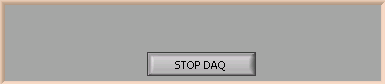
\includegraphics[width=.3\linewidth]{screenshot-stopdaq}
  \label{fig:stopdaq}}
\hfill
\subfloat[]{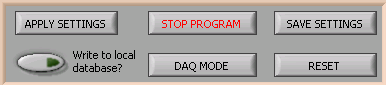
\includegraphics[width=.3\linewidth]{screenshot-applysettings}
  \label{fig:applysettings}}
\hfill
\subfloat[]{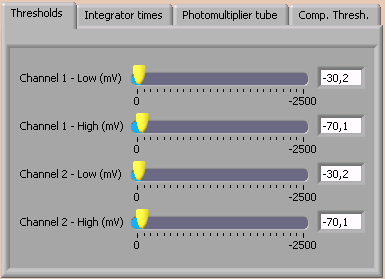
\includegraphics[width=.3\linewidth]{screenshot-drempels}
  \label{fig:drempels}}

\vspace{1em}

\subfloat[]{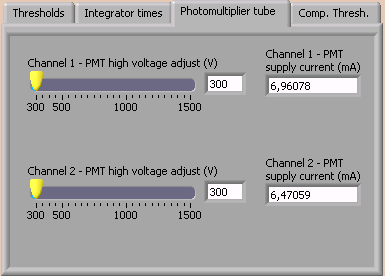
\includegraphics[width=.3\linewidth]{screenshot-spanningen}
  \label{fig:spanningen}}
\hfill
\subfloat[]{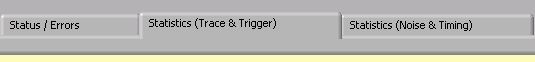
\includegraphics[width=.3\linewidth]{screenshot-tabstatistics}
  \label{fig:tabstatistics}}
\hfill
\subfloat[]{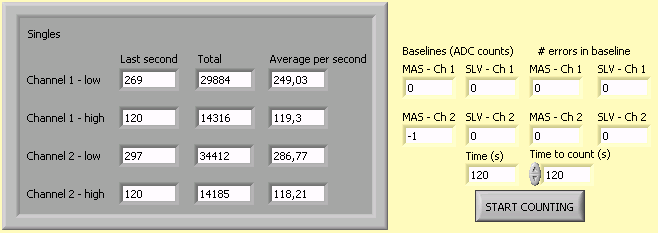
\includegraphics[width=.3\linewidth]{screenshot-counters}
  \label{fig:counters}}

\vspace{1em}

\subfloat[]{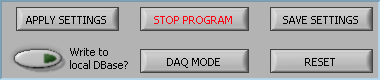
\includegraphics[width=.3\linewidth]{start-daq}
  \label{fig:startdaq}}
\hfill
\subfloat[]{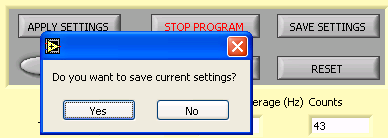
\includegraphics[width=.3\linewidth]{screenshot-savesettings}
  \label{fig:savesettings}}
\hfill
\subfloat[]{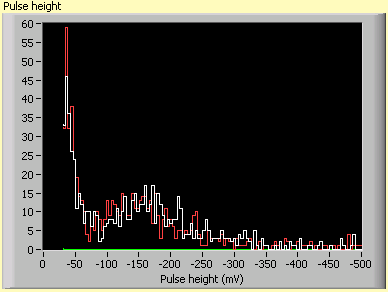
\includegraphics[width=.3\linewidth]{screenshot-histogram}
  \label{fig:histogram}}

\caption{Screenshots van de \daq software.  Deze verduidelijken de
verschillende stappen voor het inregelen van de \pmts.  Zie de
beschrijving in de lopende tekst.}
\end{figure}

De detector is nu goed afgesteld.


\begin{thebibliography}{9}
\bibitem{hamamatsu} Hamamatsu, \emph{Photomultiplier Tubes, Construction
and Operating Characteristics Connections to External Circuits} (1997).
\bibitem{9107B} ET Enterprises, Ltd., \emph{9107B series data sheet}
(2010), \url{http://my.et-enterprises.com/pdf/9107B.pdf}.
\end{thebibliography}

\end{document}
